\documentclass[letterpaper, 11pt]{article}

% Math formatting necessities
\usepackage{amsfonts,amssymb,amsmath,amsthm, mathrsfs}

% Page margins
\usepackage[left=1.5in, right=1in, top=1in, bottom=1in]{geometry}

% Adding some better options with tables
\usepackage[flushleft]{threeparttable}
\usepackage{longtable}
\usepackage{array}
%\renewcommand{\arraystretch}{1.15}
\newcolumntype{L}[1]{>{\raggedright\let\newline\\\arraybackslash\hspace{0pt}}m{#1}}
\newcolumntype{C}[1]{>{\centering\let\newline\\\arraybackslash\hspace{0pt}}m{#1}}
\newcolumntype{R}[1]{>{\raggedleft\let\newline\\\arraybackslash\hspace{0pt}}m{#1}}

\setcounter{tocdepth}{2}

% Custom colors
\usepackage[dvipsnames]{xcolor}

\definecolor{good_red}{RGB}{136, 0, 17}
\definecolor{good_blue}{RGB}{0, 100, 125}

\definecolor{color1}{RGB}{0, 143, 248}
\definecolor{color2}{RGB}{151, 165, 52}
\definecolor{color3}{RGB}{231, 105, 20}
\definecolor{color4}{RGB}{205, 182, 50}
\definecolor{color5}{RGB}{25, 102, 137}
\definecolor{color6}{RGB}{211, 186, 112}
\definecolor{color7}{RGB}{226, 126, 88}


% Formatting internal and external links
\usepackage[backref = page]{hyperref} % If you want to see what pages we cite something
\hypersetup{
	colorlinks=true,
	linkcolor= black,
	citecolor = black,
	urlcolor = good_blue
	}
\urlstyle{same}

% For images and visualizations
\usepackage{graphicx}
\usepackage{tikz, pgfplots}
\pgfplotsset{compat=1.18}
\usepackage{caption, subcaption}
\usepackage[section]{placeins}

% Citation management
\usepackage{natbib}

% Other useful packages
\usepackage{setspace} 
\usepackage{pdflscape}
\usepackage{enumitem}
\usepackage{kpfonts} % For a better aesthetic
\usepackage{dsfont}

% Custom commands
\newcommand{\cmark}{\ding{51}}
\newcommand{\xmark}{\ding{55}}
\newcommand{\fignote}[2][0.8]{\captionsetup{width=#1\linewidth, font=footnotesize, justification=justified, singlelinecheck=false}\caption*{\textit{Note}: #2}}
\newcommand{\1}{\mathds{1}}

% Formatting requirements RE: font sizes
\usepackage{titlesec}
\titleformat{\section}{\normalfont\fontsize{14}{15}\bfseries}{\thesection}{1em}{}
\titleformat{\subsection}{\normalfont\fontsize{13}{15}\bfseries}{\thesubsection}{1em}{}


% \title{Implications of Carbon Pricing for Air Pollution Disparities}
% \author{Evan Perry}
% \date{March 3, 2022}

\begin{document}

% \maketitle

\begin{titlepage}
	\centering
	{\fontsize{14}{14}\selectfont The Implications of Carbon Pricing for Environmental
	Inequality}\\
	\vspace{14em}
	by\\
	Evan Perry\\
	\vspace{10em}
	Submitted in Partial Fulfillment\\
	for Graduating with Distinction\\
	\vspace{6em}
	The Stead Family Department of Business Administration \& Economics\\
	\vspace{9em}
	Coe College\\
	Cedar Rapids, IA\\
	April 2023
\end{titlepage}

\doublespacing



\newpage
\tableofcontents

~
% \newpage
% \section*{Acknowledgements}

\newpage
\section*{Introduction}

~
\newpage
\section{Background on Climate Change \& Ambient Air Pollution}

\subsection{The Earth is Warming (and it's Our Fault)}

In its most recent report, the United Nations' Intergovernmental Panel on Climate Change (IPCC) states:
\begin{quote}
``It is unequivocal that human influence has warmed the atmosphere, ocean and land. Widespread and rapid changes in the atmosphere, ocean, cryosphere and biosphere have occurred." \citep{ipcc1_summary}
\end{quote}
This statement, which follows from possibly the single largest scientific endeavor in human history, is the first critical piece in the climate change story. Before examining why we know that human influence, particularly the burning of fossil fuels, is responsible for the observed warming, we begin by addressing the fundamentals of our current climatic situation. 

We are most familiar with weather, the day-to-day changes in temperature, precipitation, cloud cover, and severe storms. These changes are easy enough to notice by just going outside or looking the window. Climate is a long-run measurement that sizes up weather patterns. In our everyday lives, changes in the climate are much more difficult to detect. Long-run averages of the weather do not exist for anyone to simply look out a window and notice. Fortunately there is data on the day-to-day weather, meaning that with this data, anyone can calculate simple averages of temperatures and look at how climate has changed in even just the last twenty years. To the statistician, weather is a random variable drawn from a distribution, while climate is the moments of this distribution \citep{auffhammer2018quantifying}. 

\begin{figure}
\centering
\caption{The Climate is Warming \citep{ipcc1_summary}\label{ipcc1}}
\includegraphics[width=0.6\textwidth]{figures/chapter1_figures/ipcc_fig1.png}
\end{figure}

There is absolutely no question that climate change is occurring. The black line in Figure \ref{ipcc1} displays the change in global temperatures since 1850. The average global surface temperature of the 21st century is 0.99$^\circ$C warmer than the global surface temperature from 1850 to 1900 \citep{ipcc1_summary}. While finding global temperatures is more complicated than a simple average, refuting that the planet is warming amounts to questioning whether or not thermometers actually measure the temperature. The Earth is warming, and even though we cannot go outside and immediately see this, it is still an empirical reality. 

There also no question that climate change is driven primarily by human activity. The tan series in Figure \ref{ipcc1} are simulated results using both human and natural drivers of climate, and the green series are simulated results using only natural drivers of climate. These simulations comes from leading climate models which are heavily reviewed by the scientific community. Natural factors alone cannot explain the rise in global temperatures. Only when we incorporate the impact of humans into climate models does the observed warming make any sense. 

As intelligently crafted as these climate models are, they are remarkably complex. The complexity of these models makes it difficult to understand why the scientific community knows humans are responsible for the recent climate change. Before looking at how scientists attribute the changes in the climate to different factors that have the potential to influence climate, first we look at the possible causes for the climate to change. 

Climate does not change without reason. The energy that warms the Earth and controls the climate comes from the Sun. The Sun covers half of the Earth in radiation at any given time. The atmosphere and Earth reflect about 30\% of this radiation back into space. The atmosphere absorbs 19\% of this radiation, and the surface of the Earth absorbs the remaining 51\%. When absorbed by the Earth's surface, the surface emits infrared radiation, or heat. Surface heat accounts for some of the planet's warmth, but most of this actually comes from the atmosphere \citep{csi}. When the surface emits infrared radiation, this moves out into the atmosphere. Certain particles sometimes absorb this infrared radiation and send it back to the surface. We call these particles \emph{greenhouse gasses}. Greenhouse gases keeps some heat energy from leaving the planet, similar to how a blanket keeps some heat from leaving your body. This heat is not inevitably trapped on the planet, but allows the same energy to be reabsorbed by the surface before attempting to leave the atmosphere again.

The planet's global temperature is stable when the radiative energy that coming into the Earth is equal to the radiative energy that the Earth emits back into space. When the radiative energy that comes to Earth is greater than the radiative energy the leaves Earth, then this surplus energy causes warming \citep{noaa}. This imbalance that causes changes in global temperatures is called \emph{radiative forcing} or \emph{climate forcing}.

There are several major factors that impact radiative forcing: solar irradiation, volcanic eruptions, land use, aerosols, and greenhouse gases \citep{SINGH202179}. \emph{Solar irradiation} refers to the power the Sun gives to the Earth on a per unit of land basis (W/m$^2$). One important factor affecting solar irradiation is the Earth's orbit and rotation. The Earth rotates on a 23.5$^\circ$ axis currently, but over the course of millennia, the tilt of this axis changes. This change in rotation and the subsequent climatic changes are known as the Milankovitch cycles. These cycles also incorporate slight changes in the Earth's orbit that make it more elliptical, bring the planet closer to the Sun during certain periods. While this does affect climate, it does so over the course of thousands of years rather than decades. Other fluctuations from the Sun have the potential to create radiation forcing and changes in the climate over somewhat shorter periods of time. For instance, reduced solar output is a leading explanation of the period of cooler climate in Europe and North America from the early 14th century to the early 19th century, an event known as the Little Ice Age \citep{little_ice}.

Land use, volcanic eruptions, and aerosols affect the planet's \emph{albedo}, the reflectivity of the planet. Recall that the Earth reflects about 30\% of the radiation from the sun. This percentage can change based on the presence of reflective and absorbent features on the surface and in the atmosphere. Some of this reflection occurs at the Earth's surface. White ice reflects radiation, while the black pavement of roads absorbs the Sun's radiation, emitting back the heat or infrared radiation. Agricultural land is generally more reflective than dark forests. Changes in land use like these can affect how much energy the surface absorbs or reflects, and consequently change the planet's albedo and climate. 

Another way to change the Earth's albedo and climate is through aerosol concentrations. Aerosols are small solid or liquid particles in the atmosphere that are can influence cloud cover and the Earth's albedo. Around 90\% of all aerosols in the atmosphere come from natural sources including dust, sea salt, and  wildfire ash. Humans emit the remaining 10\% of aerosols. Burning coal releases sulfur dioxide and driving cars releases fine particulate matter, both aerosols. Aerosols affect climate in two ways: (1) the direct effect of either absorbing or reflecting radiation in the atmosphere, and (2) cloud formation \citep{gfdl}. Most aerosols reflect light and have a cooling effect, with the notable exception of black carbon. Black carbon absorbs light and can be particularly destructive if it coats glaciers, turning these reflective surfaces black. This is the direct effect of aerosols. The second, indirect effect of aerosols is in the creation of clouds. Clouds require aerosols in order to form. Additional aerosols in the atmosphere make cloud formation easier and can even lengthen the lifespan of a cloud. This additional cloud cover reflects radiation and keeps the surface cooler. Unfortunately many common aerosols like sulfur dioxide are dangerous for human health and create acid rain in large concentrations. 

Volcanic eruptions can also influence the planet's albedo. It is true that volcanic eruptions emit greenhouse gases like carbon dioxide. However, volcanic greenhouse gas emissions are less than one percent of all anthropogenic emissions \citep{usgs, gerlach2011volcanic}. The suggestion that higher concentrations of carbon dioxide in the atmosphere are the result of volcanic eruptions rather than human activity is utterly false. Volcanic eruptions can often have a cooling effect on the climate (negative radiative forcing). These eruptions send large quantities of sulfur dioxide, an aerosol, into the troposphere. This creates large, and long-lasting clouds that reflect solar radiation and raise the Earth's albedo. 

\begin{figure}
	\caption{Current Carbon Dioxide Concentrations are Unprecedented \citep{noaa1} \label{noaa1}}
	\centering
	\includegraphics[width=0.7\textwidth]{figures/chapter1_figures/co2_noaa.jpg}
\end{figure}

Lastly, greenhouse gases can create radiative forcing. Higher concentrations of greenhouse gases make it more likely that any infrared radiation emitted on the planet's surface will be re-absorbed by the atmosphere and continue to heat the surface. The most important and common greenhouse gas is water vapor. Water evaporates from the surface, enters the atmosphere, absorbs heat from the planet, and keeps this heat around the surface. We know from the water cycle that the quantity of water vapor in the atmosphere is a function of the current temperature. For water to evaporate, it requires some external warming. For this reason we do not see radiative forcing from water vapor---any warming that occurs as the result of additional water vapor is attributable to the radiative forcing that caused the there to be more water vapor. Water vapor is an accelerator for the warming effect of other greenhouse gases.

The most recognized greenhouse gas is carbon dioxide or CO$_2$. Carbon dioxide makes up the bulk of all human-induced greenhouse gas emissions and, other than water vapor, is the most prevalent greenhouse gas in the atmosphere. Figure \ref{noaa1} shows the concentration of carbon dioxide in the Earth's atmosphere over the previous hundreds of thousands of years. In all this time, the concentration of carbon dioxide in the atmosphere never exceeded 300 parts per million (ppm). In 2020, the atmospheric concentration of carbon dioxide reached 412.5 part per million. Historically, the increase in carbon dioxide is practically instantaneous, and this result is completely attributable to humans. Natural flucuations have played out for hundreds of thousands of years---what we see today is unprecedented and undoubtedly the result of human activity, not natural causes. Elevated concentrations of greenhouse gases can keep additional infrared radiation around the surface of the Earth, warming the world. The next section takes a closer look at greenhouse gas emissions in the US and globally. 

\begin{figure}
\centering
\caption{Warming is Driven by Human Activity \citep{ipcc1_summary}\label{ipcc2}}
\includegraphics[width=\textwidth]{figures/chapter1_figures/ipcc_fig2.png}
\end{figure}

These various sources, solar irradiance, land use, aerosols, volcanic eruptions, and greenhouse gases, represent a comprehensive list of the factors that could possibly change global temperatures like we have seen them change. From here, scientists can measure how each of these factors have changed over the period we have seen warming. Incorporating some physical constants, researchers calculate the radiative forcing of each of these factors. Figure \ref{ipcc2} displays the results of these radiative forcing studies. This makes it remarkably clear that humans are responsible for climate change. 

Natural radiative forcing from solar drivers, volcanic activity, and internal variability is not perceptible. Historically, this is not surprising. The planet has never warmed so quickly---why would natural forces suddenly cause warming unlike any other time in history? Instead we see that warming is attributable to increases in greenhouse gases like carbon dioxide, methane, nitrous oxide, and others. This warming is partially offset by increasing concentrations of aerosols. Furthermore, we know that humans are responsible for the large increases in these greenhouse gases. We call the climate change caused by humans, rather than natural forces, \emph{anthropogenic climate change}.

If we are not convinced by the calculations of scientists and researchers, observational evidence can still demonstrate the human-origins of climate change. The planet is warming, but not quite the entire planet. The lowest level of the atmosphere that humans inhabit has warmed, but the upper layers of the atmosphere that absorb radiation from the Sun have not \citep{C2ES}. If climate change was the result of some change external to the Earth, then the stratosphere would warm as well. Without any warming in the stratosphere, we know that the warming must occur from activity on the Earth's surface. Natural activities on the surface like volcanic eruptions cannot account account for changes in temperature. These factors have largely remained unchanged over the period of warming we have already encountered, and often make such small contributions to shifts in global climate that we cannot seriously attribute climate change to these factors. Simple deduction leaves human activity as the culprit of the climate crisis. The Fourth National Climate Assessment makes the summation of all these scientific observations clear:
\begin{quote}
``Global average temperature has increased by about 1.8°F [1.0$^\circ$C] from 1901 to 2016, and observational evidence does not support any credible natural explanations for this amount of warming; instead, the evidence consistently points to human activities, especially emissions of greenhouse or heat-trapping gases, as the dominant cause." \citep{nationalar4}
\end{quote}


\subsection{Greenhouse Gas Emissions: Structure \& Trends}

Anthropogenic greenhouse gas emissions drive climate change. Carbon dioxide, methane, and nitrous oxide dominate greenhouse gas emissions in the US and globally. Florinated gases, also called F-gases, make up a non-negligible proportion of greenhouse gas emissions in the US, and are growing at an alarming rate.

Not all greenhouse gases are created equal. Some greenhouse gases remain in the atmosphere longer than others and absorb more infrared radiation from the Earth than others. Greenhouse gases may also react and create different greenhouse gases in the atmosphere, which themselves can have different warming effects. To improve the accounting of greenhouse gases, researchers standardize the varied warming effect of these greenhouse gases through a measure called global warming potential (GWP). GWP measures the warming effect of other greenhouse gas emissions relative to the warming effect from a ton of carbon dioxide. For instance, in the IPCC's 5th Assessment Report, methane has a GWP of 28, meaning that a ton of methane emissions has the same warming effect as 28 ton of carbon dioxide. This metric then leads to carbon dioxide equivalent emissions, a standard unit of account for different greenhouse gas.

\begin{table}
\centering
\caption{Global Warming Potential (GWP) by Greenhouse Gas \label{gwptable}}
\begin{tabular}{l c C{4cm} C{4cm}}
	\hline
	& & \multicolumn{2}{c}{IPCC Calculated GWP  over 100 Years}\\	
	\cline{3-4}
	Gas Name & Chemical Formula & Fourth Assessment Report & Fifth Assessment Report \\ 
	\hline
	Carbon dioxide & CO$_2$ & 1 & 1 \\
	Methane & CH$_4$ &25 & 28 \\
	Nitrous oxide & N$_2$O & 298 & 265\\
	HFC-134a & CH$_2$FCF$_3$ &1,430 & 1,300\\ 
	HFC-23 & CHF$_3$ & 14,800 & 12,400 \\
	Nitrogen trifluoride & NF$_3$ & 17,200 & 16,100\\
	Sulfur hexafluoride & SF$_6$ & 22,800 & 23,500\\
	\hline
\end{tabular}\\
\smallskip

\raggedright \footnotesize
Original data from \cite{forster2007changes} and \cite{ipcc_ar5_forcing}. Table adapted from \cite{gwp_table}.
\end{table}

Table \ref{gwptable} lists the GWP for the most common greenhouse gases and a handful of F-gases as calculated under the IPCC's Fourth and Fifth Assessment Reports. Carbon dioxide is always one because it is the standard unit. Methane has a shorter atmospheric lifespan than carbon dioxide, but absorbs much more energy during this time. The agriculture industry accounts for the largest share of methane emissions, followed closely by the mining and processing of fossil fuels.\footnote{\url{https://www.epa.gov/ghgemissions/overview-greenhouse-gases}} Nitrous oxide emissions occur almost entirely from agriculture, particularly from the application of fertilizers and other soil management practices. These emissions linger in the atmosphere longer than methane and absorb heat better than carbon dioxide. The IPCC's  latests estimates indicate one ton of nitruos oxide equates to 265 tons of carbon dioxide. F-gases like HFC-134a (the most common hydroflorocarbon in the atmosphere), HFC-23, nitrogen trifluoride, and sulfur hexafluoride are rare. These gases emerged to replace chlorofluorocarbons following the Montreal Protocol. While these gases do not have quite the same ozone-destroying effect of their predecessors, they can have huge GWP in even small quantities. They tend to remain in the atmosphere for a much longer time and absorb far more energy than more common greenhouse gases. For this reason, F-gases are also often called high GWP gases.

\begin{figure}
\caption{US Greenhouse Gas Emissions 1990--2019\label{ghg1}}
\centering
\includegraphics[scale=1]{figures/chapter1_figures/ghg_stacked.png}
\end{figure}

When we put all anthropogenic emissions into a common measurement, carbon dioxide equivalent, then we can compare greenhouse gas emissions and accurately evaluate the composition of greenhouse gases and the threat of certain gases relative to others. Figure \ref{ghg1} plots total greenhouse gas emissions (in millions of metric tons of carbon dioxide equivalent, CO$_2$e) in the US from 1990 to 2019 by the offending greenhouse gas. First, US greenhouse gas emissions have fallen over the past ten years. Second, it is clear why there is so much emphasis on carbon dioxide. Carbon dioxide makes up a clear majority of all anthropogenic greenhouse gas emissions in the US. Most of the recent reductions in greenhouse gas emissions are attributable to falling carbon dioxide emissions. Although they still make up just sliver of emissions, F-gases have seen the most growth over the period, up 86.3\%. 

\begin{figure}
\caption{US Greenhouse Gas Emissions by Economic Sector 1990--2019 \label{ghgeconomic}}
\centering
\includegraphics[scale=1]{figures/chapter1_figures/ghg_economic.png}
\end{figure}

Where then are these greenhouse gases coming from? One way to answer this question is by looking at greenhouse gas emissions by economic sector. Figure \ref{ghgeconomic} plots the greenhouse gas emissions of major US economic sectors in carbon dioxide equivalent from 1990 to 2019.  The emissions reductions from electricity generation and industry have driven the most recent decline in greenhouse gases. Transportation has consistently been the largest source of emissions, making up 28.6\% of all US greenhouse gas emissions in 2019. Electricity generation makes up a slightly smaller share with a clearer path to zero emissions through the expansion of renewable electricity generation and other low-carbon intensity fuel sources. Industrial greenhouse gas emissions have fallen by just about 8\% since 1990, and 22.9\% of all US emissions were from industry in 2019. The agriculture industry contributed 10.2\% of all US emissions in 2019. Commercial and residential emissions occur mostly from burning fossil fuels to heat buildings and homes. Together, these accounted for 12.7\% of all emissions in 2019. 

\begin{figure}
\caption{US Greenhouse Gas Emissions by Inventory Sector 1990--2019}
\centering
\includegraphics[scale=1]{figures/chapter1_figures/ghg_inventory.png}
\end{figure}

The US also reports greenhouse gas emissions by inventory sector, which considers the physical sources that create and remove emissions. This can be more useful than looking greenhouse gases by economic sector if different economic sectors create emissions for similar reasons. Indeed, we see that energy generation commands the majority of greenhouse gas emissions across economic sectors. Energy makes up 82\% of gross greenhouse gas emissions in the US. This is driven by the burning of fossil fuels, releasing carbon that was trapped in the ground into the air. Agriculture and waste both make meaningful contributions, mostly through methane and nitrous oxide emissions. Hydroflorocarbons and other high GWP gases are responsible for a considerable portion of emissions that occur during industrial processes. The EPA also reports data on the nations carbon sink. Carbon dioxide cycles naturally through the environment, emitted into the atmosphere by decomposing organic matter and reabsorbed by plants life. This natural carbon sequestration creates the carbon sink. Forestry and other plant life remove emissions from the air and store them, a flow of greenhouse gas emissions out of the atmosphere. For the US to reach net zero greenhouse gas emissions, this carbon sink must be equivalent to all other greenhouse gas emissions. 

\begin{table}
\caption{US Electricity Generation by Source \label{ele_gen_source}}
\centering
\begin{tabular}{l C{3cm} C{3cm}}
\hline \hline
Energy source & Billion kWh &	Share of total \\ 
\hline 
Fossil fuels & 2,427 & 60.6\% \\
\qquad Natural gas &	1,624	& 40.5\% \\
\qquad Coal & 773 & 19.3\%\\
\qquad Petroleum	& 17 & 0.4\% \\
\qquad Other gases & 11& 0.3\% \\
Nuclear & 790	& 19.7\% \\
Renewables & 792 & 19.8\% \\
\qquad Wind & 338 & 8.4\%\\
\qquad Hydropower	& 291 &	7.3\% \\
\qquad Solar & 91 & 2.3\% \\
\qquad Biomass	& 56 & 1.4\% \\
\qquad Geothermal & 17 & 0.4\% \\
Other sources & 8 & 0.2\% \\
Total: All sources	& 4,007  & ---\\
\hline \hline
\footnotesize \raggedright Data from \cite{eia_report1}.
\end{tabular}
\end{table}

With electricity generation and energy broadly making up such a considerable portion of US greenhouse gas emissions, it is important to understand the composition of electricity generation by fuel source in the US. Table \ref{ele_gen_source} shows the fuels that drive US electricity generation. Fossil fuels make up the majority of electricity generation with 60.6\% of all electricity coming from fossil fuels. Natural gas is the single largest fuel source for US electricity generation, with more electricity from natural gas than the next two most common fuels (nuclear and coal) combined. Natural gas burns much cleaner than coal; coal emits 95.74kg of carbon dioxide per million BTUs on average while natural emits 52.91kg of carbon dioxide per million BTUs.\footnote{British thermal units (BTUs) measure thermal energy. One BTU is the amount of heat energy required to warm one pound of water by one degree Fahrenheit. \url{https://www.eia.gov/environment/emissions/co2_vol_mass.php}} Still, Figure \ref{ghgeconomic} shows that despite the low emissions intensity of natural gas relative to other fossil fuels, it is still a fossil fuel that produces significant emissions. Fuels with low carbon intensities, like nuclear and renewables, make up the remainder of electricity generation, around 40\% of all US generation.

Climate change and excess greenhouse gas emissions might be a much simpler problem to address if they were unique to the US. They are global problems, and while the US is a major emitter of greenhouse gases, it is not the only nation with significant emissions. Figure \ref{global_ghg} shows the greenhouse gas emissions by country from 1990 to 2016. China is the largest producer of greenhouse gases, followed by the US. India and the European Union currently put similar quantities of greenhouse gases in the atmosphere, but are trending in opposite directions. As India develops, its emissions are growing, while Europe's emissions are falling. We see here that just a few countries, particularly the US and China, make up a significant portion of all greenhouse gas emissions. In these countries, emissions reductions are especially important. 

\begin{figure}
\caption{Global Anthropogenic Greenhouse Gas Emissions 1990--2016 \label{global_ghg}}
\centering
\includegraphics[scale=1]{figures/chapter1_figures/ghg_international.png}
\end{figure}

Although the US is a major contributor to global greenhouse emissions, it is not the largest (second place, woohoo). When we consider greenhouse gas emissions in per capita terms though, the situation in the US seems even more imperiled. Figure \ref{global_ghg_cap} looks at greenhouse gas emissions per capita for the leading greenhouse gas contributors. The US far outpaces other developed nations. Notably, the US has more than double the greenhouse gas emissions per capita as China. The US stands out on the global stage as in terms of wealth, size, and apparent inability to reduce its greenhouse gas emissions.

\begin{figure}
\caption{2016 Greenhouse Gas Emissions per Captia of Leading Emitters \label{global_ghg_cap}}
\centering
\includegraphics[scale=.9]{figures/chapter1_figures/ghg_cap.png}
\end{figure}


\subsection{The Impacts of Climate Change}

The previous sections have demonstrated that human activity, particularly the burning of fossil fuels, is responsible for climate change. Before we start designing policy to reduce greenhouse gas emissions, we first need to understand how climate change affects us today and could affect us in the future. In this section, we discuss some of the major impacts of climate change.

First though, we should discuss how we estimate future damages from climate change. 

The overarching approach 

Before we can estimate how climate change will affect the world in the future, we have to start with assumptions about what the world will look like in the future. Given this, we then 






The goal of climate impact studies is to estimate how emissions today and in the future will lead to a climatic scenario and then estimate how that climatic scenario will ripple through different ecosystems, communities, and economies. Economists often take this a step or two further, and try to put all of the costs (and benefits) of climate change into economic terms and then tie these prices into present terms. This gives the foundation for the the social cost of carbon [CITATION, https://www.rff.org/publications/explainers/social-cost-carbon-101/]. For our present purposes we do not need to relate all of these impacts back into prices, so we will omit a more detailed description of the social cost of carbon for now. 

The inputs to these climate impact models are known as emissions pathways. Despite the name, emissions pathways do not truly map out different emissions scenarios, but different concentrations of greenhouse gases alongside certain socioeconomic assumptions. A simplified emissions pathway might assume a certain time series of greenhouse gas concentrations, human population, and GDP over the century. The Intergovernmental Panel of Climate Change (IPCC) has standardized two collections of emissions pathways: Representative Concentration Pathways (RCPs) and Shared Socioeconomic Pathways (SSPs).\footnote{Often you might see something such as ``RCP$_{4.5}$" or ``SSP$_{8.5}$." The numeric subscript indicates the amount of radiative forcing the emissions scenario creates by 2100. For instance, RCP$_{4.5}$ will lead to 4.5 W/m$^2$ of radiative forcing---a measure of the average energy absorbed by the planet. Similarly, SSP$_8.5$ creates 8.5 W/m$^2$ by 2100, and is often used as the ``do nothing" response to cliamte change [CITATIONS, AR6 SPM]} Climate models then assume these scenarios and map out what the climate looks like over the course of the century using these 

% - Something about General Circulation Models (GCMs?)?
% - What are the CMIP things?

Process-based models suffer in in important ways. First, they are computationally intensive. 



While these process-based models create the backbone of impact estimates, economists often opt to use simpler method for mapping climatic outcomes to quantitative impacts called damage functions. Damage functions are reduced-form estimations of the relationship between climate variables (e.g. average surface temperatures) and impact variables of interest (e.g. mortality rates). That is, damage functions do not attempt to explain the complex systems that give rise to these damages and focus instead on just explaining aggregate impacts. For instance, [CITATION] create straightforward damage functions for the US by using process-based impact models to generate estimates of climate change impacts (in monetary terms) under a variety of climate scenarios. Then they use OLS to estimate the relationship between surface temperature measurements and the monetary value of climate change impacts. The estimated model is a damage function, mapping changes in surface temparatures to impacts. Damage functions like this and many others provide useful tool in a variety of applications, especially in calculating the social cost of carbon. 

\cite{auffhammer2018quantifying} notes that perhaps the greatest difficulty in using damage functions to map climatic scenarios into physical impacts is accounting for adaptation. Although it would be much easier to assume that people and businesses . \cite{auffhammer2018quantifying} uses the example of an air conditioner. Suppose we are interested in the impact of a changing climate on electricity use. We expect there to be more hot days, meaning that people will run their air conditioners more frequently and use more electricity to do so. This response on the intensive margin is measurable; we have the data to estimate how people use their air conditioners differently when it is warmer outside. The extensive margin cannot be realiably measured. 
We do not have reliable measurements for how many more people will purchase and use air conditioners after decades of sustained warming.\footnote{A promising but limited approach to studying climate change adaptation is by estimating how people have adapted to climate changes in the past. For instance, [CITATION, Drunkenmiller] are using historical aerial photographs of Western Africa to study land use and migration changes that occurred as a result of drought during the mid-twentiwth century.}

Admittedly, there is a considerable amount we still do not know about the impacts of climate change. Truthfully, we are not exactly sure how the estimated 3.3 to 3.6 \emph{billion} people who are highly vulnerable to climate change will adapt [CITATION]. Will hundreds of millions of people living in some of the most impoverished corners of the planet seemlessly migrate en masse to places with more hospitable climates over the course of just a few decades? 

What we do know is that today, our best estimates indicate that the impacts of climate change are frightening. 

In the preceeding subsections, we look at the

The IPCC outlines five major ``reasons for concern" regarding climate change:
\begin{enumerate}
	\item Unique and threatened systems
	\item Extreme weather events
	\item Distribution of impacts
	\item Global aggregate impacts
	\item Large-scale singular events
\end{enumerate}
These represent some of the most important risks that we face from climate change. 

% intramarginal vs. extramarginal

\subsubsection*{Unique \& Threatened Systems}

While many systems---both natural and social---face steep challenges from climate change, some of these face complete ruin. Many of the most vulerable systems are endemic. Endemism refers to species, cultures, and resources that are restricted to specific geographic areas. [CITATION] In a changing climate, systems that are tied to specific regions and climates risk extinction if they cannot plausibly adapt. This includes the extinction of species whose habitats are destroyed by climate change, 
the death of indigenous cultures that are highly dependent on the climate, and the destruction of historical artifacts and landmarks. Unfornately in each of these cases, the affected system cannot is unique and we could not replace it for the remainder of human existence. These kind of consequences do not fit well into standard economic understanding of sustainability. \footnote{*Talk about an economic definition of sustainability from Romer, and why it might not be able to capture some of the threats of climate change well.*}


\subsection{The Impacts of Ambient Air Pollution}

\textit{Forthcoming}.


\subsection{A Review of Air Quality Disparities}

\textit{Forthcoming}.



%%%%%%%%%%%%%%%%%%%%%%%%%%%%%%%%%%%%%%%%%%%%%%%%%%%%%%%%%%%%%%%%%%%%
%\subsection{The Impact of Climate Change}
%
%At this point we have covered why we know climate change exists, why we know humans are responsible for climate change, and what the composition of greenhouse gas emissions look like. We have to to justify why anyone should care about climate change though. Here, we take a brief and high-level examination of the impacts of climate change. If I had to summarize the magnitude of climate impact estimates by even just the end of the century, I would probably say that they lie somewhere in between pretty bad to borderline apocalyptic. 
%
%Admittedly, the impacts of climate change on natural ecosystems and society are not understood quite as well as the causes of climate change. This gap in knowledge is closing as we collect new data on the impact of the climate change we have already seen. The IPCC summarizes these impacts in its Fifth Assessment Report in five ``reasons for concern." These reasons for concern relate to:
%\begin{enumerate}
%	\item Unique and threatened systems
%	\item Extreme weather events
%	\item Distribution of impacts
%	\item Global aggregate impacts
%	\item Large-scale singular events
%\end{enumerate}
%
%There are certain physical elements of the natural and built environment that are unique and irreplaceable. Losing these due to climate change poses a significant cost for all future generations. For instance, warming waters threatens coral reefs. With sustained and substantial warming, the world's coral reefs could be permanently destroyed. Many important historical sites are located in low-lying coastal areas threatened by rising sea levels from climate change. Climate change has the power to permanently destroy many of the ecosystems we cherish and other culturally significant creations.
%
%Extreme weather events pose the greatest This includes a greater frequency of severe but short-lived weather events, like tornadoes or monsoons. More concerning is are sustained heat-stress events. As Freddy's mom from iCarly once said, ``when temperatures get too high, the elderly will start to die" (a rather creepy but fitting rhyme). Elevated temperatures can induce cardiovascular events, particularly in vulnerable populations like the poor, elderly, and those who work outside. Sustained events like this can trigger droughts and resulting in famine. Higher humidity can bolster mosquito populations and allow blood-borne infectious disease to spread easier. Extreme and sustained events like these pose serious challenges to public health.
%
%Related to this, impacts tend to fall most severely on populations who are already at the greatest disadvantage. Some of this is simply due to geography. Climate predictions for the African continent are sickening. Much of this is due to adaptation costs. When it is 110$^\circ$F outside, the well off do not just sweat---they run their air conditioners on full blast. This is not true of the global poor, who cannot afford to pay to adapt to rising temperatures, and instead suffer the heat and risk death. 
%
%Global impacts on natural life and the economy are not well understood, but what we know is not reassuring. The economic impacts of climate change will become much more apparent as concentrations of greenhouse gases increases. That is, the economic damages from climate change are increasing at an increasing rate with the concentration of greenhouse gases. There is some additional concern about low-probability, highly dangerous climate change-induced events. 
%
%\begin{figure}
%	\caption{Climate Change Damages by Income \& Climate \citep{carleton2020valuing} \label{cil1}}
%	\centering
%	\includegraphics[width = \textwidth]{figures/chapter1_figures/cil_dist.png}
%\end{figure}
%
%\begin{figure}
%	\caption{The Climate Change Mortality Rate \citep{carleton2020valuing} \label{cil2}}
%	\centering
%	\includegraphics[width = 0.8\textwidth]{figures/chapter1_figures/cil_mortal.png}
%\end{figure}
%
%Figures \ref{cil1} and \ref{cil2} depict estimates of moralities by end of the century from climate change induced events. These summarize many of the most important takeaways from the impacts of climate change. Those who live in poor and warm areas will suffer the most from climate change. The mortality rate from climate change is comparable to the mortality rate of other leading causes of death. Overall, the situation climate change poses by just the end of the century is extremely grim and warrants sweeping action.
\section{Designing Climate Policy}

\subsection{A Case for Economic Analysis in Climate Policy Design \label{2.1}}

This chapter shifts the discussion from describing climate change to describing the policy tools available to address climate change. Before delving too far into this topic, it is worth contemplating why the economics discipline has any role at all in the design of climate solutions. While the physical sciences have alerted the world to the destructive potential of climate change and occupy a central role in developing the abatement technologies needed to mitigate climate damages, economically-motivated actors have largely been the perpetrators of the greenhouse gas emissions responsible for climate change. Given this narrative, it is reasonable to question why economics deserves a place in designing climate solutions.  After all, why should we care about money when the fate of the planet is at risk?

The objective of this section is to address these concerns and motivate the use of economic analysis in climate policy design.  This starts by summarizing some of the key perspectives that the economics discipline can contribute to the study of climate policy and climate solutions. From there, the section closes by clarifying a few key ways that the economics discipline understands the environment and climate change in particular. 

First and foremost, it is important to establish that economic analysis should not and cannot hope to address climate change without other disciplines. There is a tremendous need for scientific research into technical solutions with the potential to reduce greenhouse gas emissions. In the International Energy Agency's plan to achieve net zero emissions by 2050, currently available technologies can only sustain abatement through 2030. By 2050 only half of the technology needed to reduce emissions is currently on the market. The agency estimates that governments worldwide will need to immediately invest over \$90 billion into key areas of research and development like electrification and carbon capture technologies---areas that currently receive only about \$25 billion in research funding \citep{ieareport}. Not only does the world need the efforts of the physical sciences to address climate change, but economists do for their own work as well. As discussed in section \ref{scc_section}, the damage functions economists use to estimate the costs of climate change necessarily rely on the physical sciences to build the underlying climate models. Clearly, economic analysis alone cannot guide climate policy design. 

Still, physical science alone cannot hope to address climate change without the perspective of the social sciences, including economics. The discipline makes two key contributions to the study of climate policy: (1) a broader perspective on the impacts of both climate change and climate policy, and (2) an understanding of the social mechanisms that lead to greenhouse gas emissions. 

The previous chapter addressed the impacts of climate change---an area of study that relies heavily on both the work of physical scientists and social scientists.  Ultimately though, making climate policy decisions requires an understanding of how these policies affect the people they intend to protect, not just an understanding of the impacts of climate change. To clarify this point, consider an example where a small, credit-constrained  government must decide how to allocate tax revenue. There are many important and worthwhile causes that this government could dispense funds towards. Investing in public education, improving transportation infrastructure, and improving water quality are all socially valuable, but a mandate to cut greenhouse gas emissions could force this government to devote a substantial amount of funds for these causes towards building a wind farm to replace the local coal power plant. This could be a perfectly good decision if the government in mind is a city in a high-income nation with already well-funded public education, transportation, and water quality. Of course this could be a perfectly terrible decision if the government in mind is a city in a low-income nation with nearly non-existent public education, failing transportation infrastructure, and little water security. Social and economic context is important in these decisions, and though they have many merits, the physical sciences cannot provide this context. The IPCC has identified climate change as threatening standards of living, key infrastructure, and water security (see the discussion of the Representative Key Risks in section 1.3.1). Climate policy made without any consideration of forgone public education, infrastructure upgrades, or water quality improvements runs these same risks. This does not mean that  climate policy is not worthwhile---it is---but that climate policy made without any consideration of its full costs and benefits risks unnecessary harm to the very people it is intended to protect. 

\cite{nordhaus2019climate} says this more pointedly in his Nobel lecture:
\begin{quote}
	\singlespacing ``However attractive a temperature target may be as an aspirational goal, the target approach is questionable because it ignores the costs of attaining the goals. If, for example, attaining the 1.5°C goal would require deep reductions in living standards in poor nations, then the policy would be the equivalent of burning down the village to save it."
\end{quote}
In his quote, Nordhaus does not question the need for climate policy, but emphasizes that policy decisions must be made with the underlying social systems in mind, not just the physical systems. If the goal of climate policy is to prevent declines in the quality of life, then policy decisions must include all of the ways that climate policy might impact the quality of life. Although there is room to criticize the approaches economists use to measure and model quality of life, the economics discipline is ultimately far better equipped for this task than the physical sciences. Economists generally try to quantify these costs and benefits towards the quality of life and place them in terms of a common unit, the dollar.\footnote{Expressing costs and benefits in terms of dollars is often  convenient though not necessary. For instance, in Figure \ref{cil_mortality}, \cite{carleton2022valuing} express climate change adaptation costs not in dollars, but in terms of ``statistical lives."} This quantification allows for consistent comparisons and has the advantage of clear integration with the work of climate scientists. Again, there is room to criticize the methodologies economists use in cost-benefit analysis,\footnote{It should also be acknowledged that the cost-benefit analysis foundational to economics is not without its weaknesses. Cost-benefit analysis has particular difficulty handling the highly unequal effects of climate change \citep{kaufman2022how}. Economists have developed techniques to incorporate distributional effects into cost-benefit analysis that typically involve weighting costs and benefits as they enter the summation, but these techniques are hardly standard practice. Incorporating the distribution of costs and benefits into standard analyses will undoubtedly be an important area of growth in the future of the discipline.}  but fundamentally, the ``dollars-and-cents'' talk of climate economists is focused on understanding how climate change and climate policy impacts peoples' quality of life. While the physical sciences play an indispensable role in climate policy design, economics is uniquely positioned to provide quantified assessments of the full costs and benefits of climate policy---assessments that would be valuable to any benevolent social planners.

Related to this earlier point, economics also provides a unique toolkit for analyzing the social mechanisms that lead to greenhouse gas emissions. Correcting our social and economic systems so they are mindful of the climate first requires that we have an accurate understanding of our social and economic systems. The mathematization of economics allows these explanations to easily translate into forecasts. By first understanding why we emit greenhouse gases, we can also predict what would happen to our greenhouse gas emissions if a policy change were implemented. This is the approach taken in Chapter 4 and 5 of this text. Physical sciences that omit the social and economic motivations that drive greenhouse gas emissions risk creating policy that fails entirely to reduce these emissions. 

The use of cost-benefit analysis to consider the broader economic context of policy and the use of economic modeling to anticipate how agents will respond to policy changes both constitute valuable additions to climate policy discourse. While there are certainly other and more specific ways for economists to contribute to the design of climate policy, these represent broad perspectives and genres of analysis that economics is uniquely capable of delivering. 

For the reader still critical of the use of economic analysis to study climate policy, it is important to clarify the relationship between the economics discipline and climate change. Start by considering an important question that all economists loathe: ``how is this economics?'' The archetypal economist studies topics like the stock market, inflation, unemployment, and taxes---not climate change. In reality, economists study an incredibly wide range of topics including crime, space exploration, gender reforms, and of course, climate change. At its core, economics is a social science, and as such, economists study a wide variety of social issues. Some of these social issues like financial regulation or unemployment insurance absolutely fit the popular conceptualization of economics. It turns out though that many of the tools economists use are well-suited to study social phenomena that are not so clearly connected to money. Uniting all of these seemingly disparate topics is a concern for human welfare. Financial regulation is only a valuable topic of study to economists in the sense that improvements in financial regulation can translate into greater economic stability and presumably a higher quality of life. By the same merit, environmental regulation and climate policy are a valuable topic of study to economists in that protecting our environment and climate can prevent needless declines in the quality of life. Climate change is as worthy of economic study as any of the topics that we would usually consider economics.

Second, it is worth clarifying the consensus view of economists on climate change. Economists overwhelming believe in anthropogenic climate change and believe in the need for serious policy to address it. In an open letter first published in the Wall Street Journal in 2019, twenty-eight Nobel Laureates in Economics, four former Chairs of the Federal Reserve, and fifteen former Chairs of the Council of Economic Advisors all called for the implementation of a nationwide carbon tax---a policy intended to reduce greenhouse gas emissions and mitigate the damages of anthropogenic climate change. Thousands of other economists have since signed the open letter. This chapter discusses additional details on this variety of policy, and Chapter 3 discusses the letter itself in greater detail. While the letter does not go as far as to state what this tax should be (a higher tax would correspond with more aggressive action), this letter easily dispels any myth that contemporary economists are largely climate change deniers and apologists. In a 2021 survey of climate economists, 74\% said that climate change necessitates ``immediate and drastic action." Less than 3\% answered that either ``more research is needed before action is taken" or that climate change ``is not a serious problem" \citep{howard2021gauging}.\footnote{Another 24\% said that ``some action should be taken now" on climate change.} Although it may seem trivial to some to assess the costs and benefits of climate policy, the calculus of economists adds further credibility to the case for climate policy, particularly when much of the criticism lodged at climate action centers on its cost. 

As a final rejoinder, it is worth addressing the relationship between the climate and the economy itself. There is a purported tension between mitigating climate change damages and protecting the economy---a narrative that suggests the economy and environment are fundamentally at odds and elevating the environment requires us to set aside our economic interests. This is false. To see why, consider a simplified example. Suppose the cost of eliminating all anthropogenic greenhouse gas emissions and putting a stop to all future climate change is a one time payment of \$100. Further, suppose that by putting a stop to climate change, societal welfare increases an extra \$1 every year. Absent any additional elements to this example, cost-benefit analysis will suggest that society puts a stop to climate change today. The costs are finite (\$100) but the benefits are infinite ($\$1  + \$1  + \$1 + \ldots$), so it does not matter if the cost to avoid climate change is \$100 or \$100,000,000, the benefits of climate action will always be greater than the immediate costs. At the heart of this is the understanding that the economy exists within the natural environment, and because of this, causing irreversible damage to the environment results in perpetual damage to the economy. That is, when we destroy the environment, we destroy our economy as well. 

This is not to say that there is no tradeoff involved in climate policy. Looking back at the earlier example, the complication is of course that we generally do not value costs incurred tomorrow as much as we value costs incurred today. For instance, if \$1 today is worth \$0.98 next year, then suddenly the costs become finite ($\$1  + \$0.98  + \$0.98^2 + \ldots = \$50$) and the decision is no longer trivial. Again, the discount rate is an extraordinarily powerful number. Although this thought exercise cannot provide any conclusions without realistic data, it does lead to an important distinction: economists do not analyze ``climate versus economy'' tradeoffs, but ``welfare today versus welfare tomorrow" tradeoffs. The tension is not between the environment and the economy, but between the world today and the world tomorrow. 

In summary, economics provides a quantitative and systematic approach to making potentially difficult decisions related to our relationship with the Earth's atmosphere and our environment. This approach is not without its flaws, but it is one of many important perspectives. Not only does economic analysis allow us to consider the tradeoffs of specific policy proposals, but it provides theory and empirical techniques essential to identifying how firms and individuals will respond to policy. Climate economists widely agree that climate change urgently deserves bold public policy, a view that aligns with climate scientists and researchers at large. While physical scientific research can develop the technologies that permit emissions reductions, research in economics and other social sciences will be integral in the development of policies that will integrate this technology into everyday life.


% There is a purported tension between mitigating climate change damages and protecting the economy---a tension that I discuss in greater detail later in this chapter. This belief that the economy and environment are fundamentally at odds might lead to the impression that elevating the environment must be done without regard to the economy. If nothing else, the cost-benefit analysis that underlies much of the economics discipline feels inappropriate when it comes to environmental issues. 


\subsection{An Economic Motivation for Climate Policy \label{2.2}}

% The general approach advocated by policymakers begins by making the production of electric power less carbon intensive. This involves the familiar steps of switching from coal power plants, to wind and solar farms. This is called \emph{decarbonization} of the electric power grid. Simultaneously, policymakers need to transition energy-using activities to rely on electric power, rather than other forms of energy. Electric vehicles are the most popular push for electrification. Some greenhouse gas emissions are likely inevitable, so bringing the world to net zero emissions requires that those emissions are offset through increased carbon sequestration, the removal and storage of CO$_2$ emissions from the atmosphere. The tree is a simple carbon sequestration device, but difficult to use at the necessary scale. Carbon sequestration technology requires significant public investment, but unlike decarbonization and electrification, this does not need to involve many economic actors.

The first chapter established anthropogenic greenhouse gas emissions as the culprit behind climate change, but this still leaves open questions surrounding the social and economic motivations behind these emissions. Any public policy aimed at reducing greenhouse gas emissions must first reconcile with why those greenhouse gas emissions exist in the first place. Moreover, despite having established that economics as a discipline deserves a role in climate policy design, it is worth considering whether or not public policy is necessary to address climate change at all. The objective of this section is to fill in these holes and provide an economic interpretation for both why climate change happens and why climate change is not likely to improve in the absence of public policy. This section uses foundational elements of economic theory to answer two questions: (1) why do individuals and firms release greenhouse gases into the atmosphere, and (2) can we prevent future climate change without public policy? 

To the economist, climate change is the consequence of the \emph{universal} nature of greenhouse gas emissions. Greenhouse gas emissions  are a textbook example of an externality: a cost or benefit borne by an agent who is not involved in the economic transaction that creates the cost or benefit. Consider a driver with a gasoline-fueled car. Overall, burning gasoline creates greenhouse gas emissions that lead to anthropogenic climate change which would harm the average driver. The transaction between the driver and pump creates costs that are universal, borne by everyone on the planet, a textbook example of an externality. When this driver buys and burns a gallon of gasoline in her car, she damages the climate by a non-negligible amount. In fact, a quick back-of-the-envelope calculation would suggest a central estimate for the cumulative damages associated with this gallon of gasoline of about \$1.64.\footnote{The \cite{epa2022greenhouse} finds that burning a gallon of gasoline in the average passenger vehicle creates 8887 grams of CO$_2$ emissions. Using a SCC of \$185 per tonne, as in \cite{rennert2022comprehensive}, this implies the social cost of burning a gallon of gasoline of 
$$\frac{8887 \text{g CO$_2$}}{1 \text{gallon gasoline}} \cdot \frac{1 \text{tonne CO$_2$}}{10^6 \text{g CO$_2$}} \cdot \frac{\$185}{1 \text{tonne CO$_2$}} \approx \frac{\$1.64}{1 \text{gallon gasoline}}.$$
Note also that this best thought of as a lower bound on true social damages, as this does not consider damages associated with the ambient air pollution emissions.} However, this cost is not borne by the driver alone, but distributed over the other eight billion people on the planet and even over the billions of people not yet born who will be affected by this decision in the future. Despite the additional or marginal damages from this gallon of gasoline of \$1.64, the climate damages that the driver faces herself for buying and burning this gallon of gasoline are effectively zero. If for instance, we simplified the situation to consider only damages that accrue to those eight billion people currently alive and assume that this driver experiences the average damages of all individuals, then her private cost of the associated emissions is approximately \$1.64/8 billion $\approx 0$. As a result, the price this driver pays for a gallon of gasoline is just the price at the pump. Economic theory posits that because the driver's costs do not reflect the universal costs of her emissions, she will end up consuming more of this good than what would be socially optimal.

% For any individual driver, the impact of burning one more gallon of gasoline on the climate is entirely negligible, and the cost she incurs for that next gallon of gasoline is just the price she pays at the pump. Unfortunately, she is not the only person who incurs the costs of the induced climate change---so do the other eight billion people on the planet.\footnote{There are additional externalities here related to how this activity will affect future generations. The extraction of the oil for gasoline production prevents future generations from extracting and using that same unit of oil. Future generations will also feel the climate effect caused by present emissions. In both cases, the value of these damages are highly dependent on the assumed discount rate. These are known as intertemporal externalities \citep{keohane2016markets}.} 
% However, she does not face the burden of climate change damages incurred by all other people caused by her driving. These costs are external to the driver when she chooses how much gas to put in her car or what car to buy in the first place. 

\begin{figure}
	\caption{Market for an Emissions-Intensive Good \label{mkt_ei_good}}
	\centering
	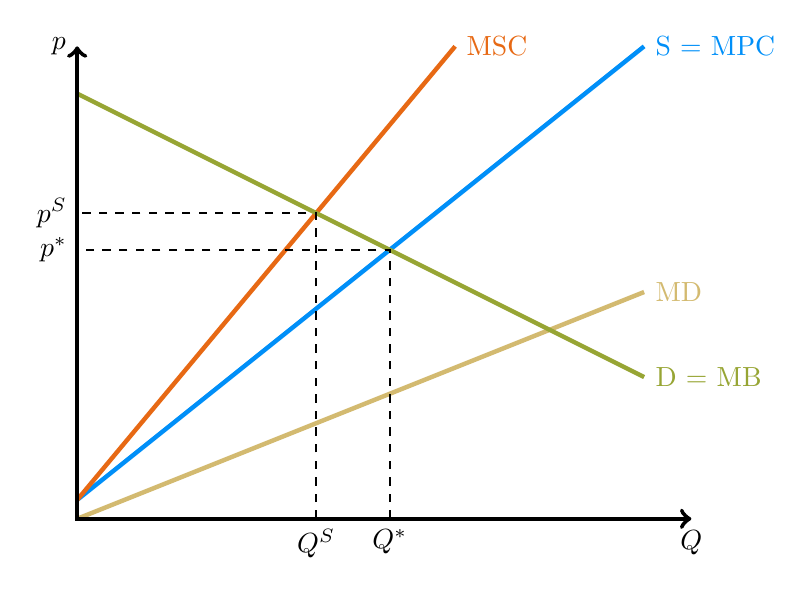
\begin{tikzpicture}[scale=0.6]
		\draw[ultra thick, color1, domain=0:12] plot (\x, {.8*\x + .4}) node[right]{S = MPC};
		\draw[ultra thick, color6, domain=0:12] plot(\x, {.4*\x}) node[right]{MD};
		\draw[ultra thick, color3, domain=0:8] plot(\x, {1.2* \x + .4}) node[right]{MSC};
		\draw[ultra thick, color2, domain=0:12] plot (\x, {-.5*\x + 9}) node[right]{D = MB};
		\draw[thick, dashed] (6.615, 0) node[below]{$Q^*$} -- (6.615, 5.692) -- (0, 5.692) node[left]{$p^*$};
		\draw[thick, dashed] (5.059, 0) node[below]{$Q^S$} -- (5.059, 6.471) -- (0, 6.471) node[left]{$p^S$};
		\draw[ultra thick, <->] (0,10) node[left]{$p$} -- (0,0) -- (13,0) node[below]{$Q$};
	\end{tikzpicture}
	\fignote[1]{Figure depicts a standard market for an emissions-intensive good, such as gasoline. In the figure, $p$ denotes the price of the good, $Q$ denotes the quantity of the good, D denotes demand, S denotes supply, MB denotes the marginal benefit associated with consumption, MPC denotes the marginal private cost associated with production, MD denotes the marginal damages stemming from the associated greenhouse gas emissions at a given quantity, and MSC denotes the marginal social cost---the sum of the marginal damages and the marginal private cost. In this case, we assume that marginal damages are increasing in $Q$, reflecting the accelerating disruptions caused by elevated greenhouse gas concentrations in the atmosphere.}
\end{figure}

Figure \ref{mkt_ei_good} depicts a generalized version of this situation diagrammatically via the market for an emissions-intensive good. As in any standard market, the market for an emissions-intensive good relates the quantity of this good ($Q$) to its price ($p$). The effective components of the market are the downward-sloping demand curve (D), and the upward-sloping supply curve (S). Here, consumers demand the good such that the price they will be willing and able to pay for an additional unit of the good is equivalent to the additional or marginal benefit (MB) they receive from consuming it, hence why D $=$ MB. Similarly, producers supply the good such that the price they will be willing and able to sell an additional unit of the good at is equivalent to its marginal private cost (MPC), hence why S $=$ MPC. Together, the demand and supply for the emissions-intensive good lead to an equilibrium price and quantity of $p^*$ and $Q^*$ respectively. 

Outside of the market though, the production and consumption of the emissions-intensive good produces greenhouse gas emissions, which lead to climate change and associated damages to others. The upward-sloping marginal damages curve (MD) depicts the cost of these emissions for each additional unit of the good. As in the previous example, these damages accrue to society at large, but not to the individual involved in the transaction. The marginal social cost (MSC) considers the full scope of costs associated with the emissions-intensive good, summing the marginal private costs and the marginal (social) damages. Total welfare in the market is maximized when the marginal social cost is set equal to the marginal benefit, an unreached equilibrium at $Q^S$ and $p^S$. Note that for an emissions-intensive good, the socially-optimal price is higher than the equilibrium price and the socially-optimal quantity is less than the equilibrium quantity. That is, the market will under-price and over-produce an emissions-intensive good. The concept of externalities provides an economic explanation for why society creates excessive greenhouse gas emissions that lead to climate change. 

It is worth considering then why---if the atmosphere is in fact so valuable---there is no market for clean air. Modern economic theory classifies goods according to two criteria: rivalry and excludability.\footnote{\cite{ostrom2010beyond} reviews the historical development of the four goods commonly used today. The seminal paper \cite{samuelson1954pure} moved the discipline away from just private goods and described a public good, introducing the excludability criterion. Although \cite{hardin1968tragedy} popularized the concept of rivalrous goods, club goods were first formally introduced in \cite{buchanan1965economic} and open-access goods were first formally introduced in V. Ostrom and E. Ostrom (\citeyear{ostrom1977public}).} A good is rival if one agent's consumption of the good inhibits another agent's consumption of the good, or is non-rival if one agent's consumption of the good does not inhibit the consumption of any other agents. Concert tickets, for example, are a rivalrous good---one person holding a ticket prevents another person from holding that same ticket. A good is excludable if it is reasonably easy to prevent someone from using it. Video subscription services are excludable, as a service can always prevent a person from accessing the service if, for instance, he stops paying his bill. If we accept the double dichotomies of a good being either rival or non-rival and excludable or non-excludable, then these criteria lead to four types of economic goods: private goods (excludable and rival), public goods (non-excludable and non-rival), open-access goods (non-excludable and rival), and club goods (excludable and non-rival).\footnote{Here I choose to use the term ``open-access good'' rather than ``common-pool resource,'' a term more common in work such as \cite{ostrom1990governing}. The intention of this choice is to clarify the non-excludability of this class of goods. A common-pool resource might be shared by a group of agents, but still excludable to others outside of this group. For instance, \cite{ostrom1990governing} considers a community forest in the Swiss Alps where the right to fell timber in the community forest was restricted to certain land owners who could prevent others from purchasing land that would grant them the timber rights. The term ``open-access good'' more clearly describes a good that is available to any interested actor but still rival (e.g., using the swing set at a public park).} The goods matrix in Figure \ref{goods} summarizes these four types of goods.

\begin{figure}
	\caption{A Taxonomy of Goods}
	\label{goods}
	\centering
	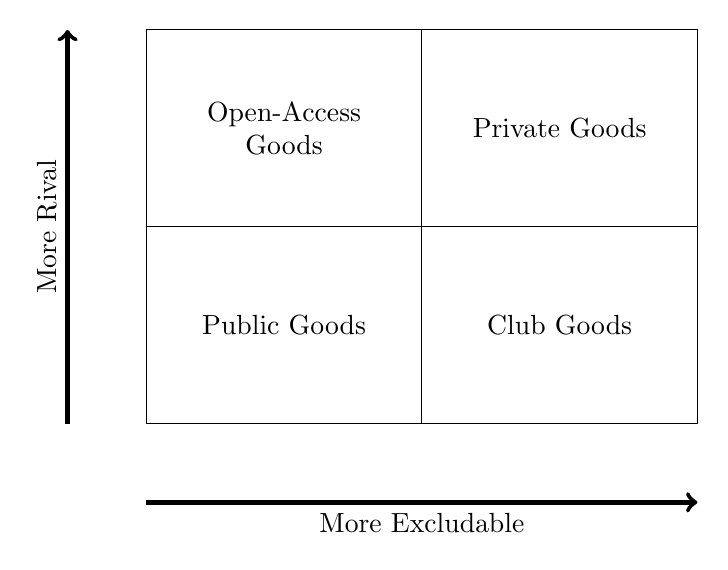
\begin{tikzpicture}[scale = 0.5]
		\draw (0,0) rectangle (7,5) node[pos=.5] {Public Goods};
		\draw (7,5) rectangle (14,10) node[pos=.5] {Private Goods};
		\draw (0,5) rectangle (7,10) node[pos=.5, text width = 2.7cm, align=center] {Open-Access Goods};
		\draw (7,0) rectangle (14,5) node[pos=.5] {Club Goods};
		\draw[ultra thick, ->] (0,-2) -- (14, -2) node[pos =.5, below]{More Excludable};
		\draw[ultra thick, ->] (-2, 0) -- (-2, 10) node[pos =.5, above, rotate=90]{More Rival};
	\end{tikzpicture}
	\vspace{1em}
	\fignote[1]{The goods matrix depicts the four main types of goods: private goods (excludable and rival), public goods (non-excludable and non-rival), open-access goods (non-excludable and rival), and club goods (excludable and non-rival). Although these are cannonically presented in four categories, the excludability and rivalry of goods is best thought of as taking place on a continuum.
	}
\end{figure}

A clean atmosphere is firmly a public good. There is no way to prevent people from benefiting from a healthy atmosphere with greenhouse gases at a level that supports climate stability, and one person's benefit does not infringe on another's. By the same virtue, greenhouse gas emissions are a public bad. No individual can exclude herself from climate change, and one person's climate damages do not prevent someone else from also experiencing those same damages. 

Defining a clean atmosphere as a public good provides a grounded explanation for why socially efficient greenhouse gas emissions abatement is unlikely to occur in the absence of public policy. All public goods struggle to find buyers. This lack of buyers is not necessarily because few people are willing and able to pay for the public good, but because these people do not have the proper incentives that would motivate them to actually buy into the public good. To see this, suppose there are two cities $A$ and $B$ on either side of a lake that is currently polluted and covered in algae blooms. Both cities benefit from the clean water in the lake through greater aesthetic appeal, higher property values, and increased ecotourism. As we have described it, clean water in the lake is a public good. Neither city can exclude the other from enjoying the clean water and one city's enjoyment of the clean water does not inhibit the other city from enjoying the clean water. 

\begin{figure}
	\caption{Market for a Public Good \label{mkt_public_good}}
	\centering
	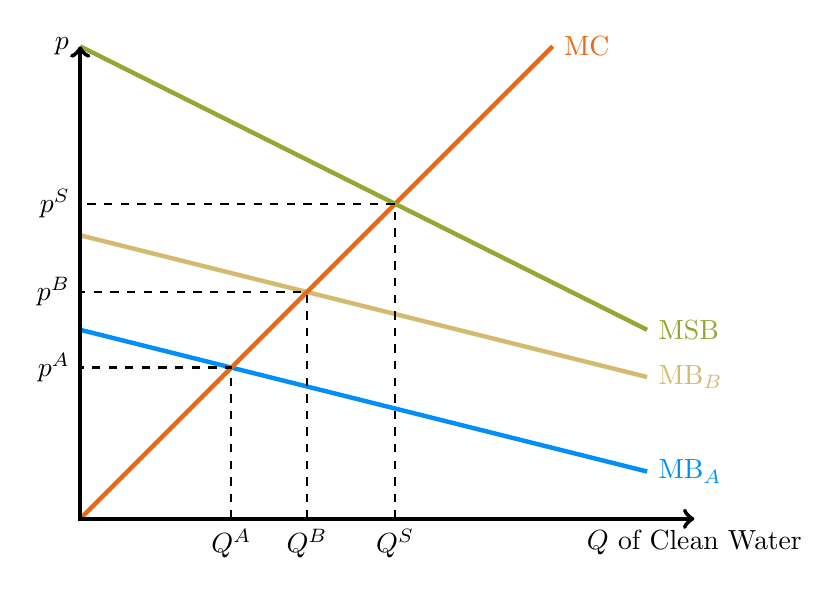
\begin{tikzpicture}[scale=0.6]
		\draw[ultra thick, color1, domain=0:12] plot (\x, {4 - .25*\x}) node[right]{MB$_A$};
		\draw[ultra thick, color6, domain=0:12] plot(\x, {6 - .25*\x}) node[right]{MB$_B$};
		\draw[ultra thick, color3, domain=0:10] plot(\x, {\x}) node[right]{MC};
		\draw[ultra thick, color2, domain=0:12] plot (\x, {10 - .5*\x}) node[right]{MSB};
		\draw[thick, dashed] (3.2, 0) node[below]{$Q^A$} -- (3.2, 3.2) -- (0, 3.2) node[left]{$p^A$};
		\draw[thick, dashed] (4.8, 0) node[below]{$Q^B$} -- (4.8, 4.8) -- (0, 4.8) node[left]{$p^B$};
		\draw[thick, dashed] (6.667, 0) node[below]{$Q^S$} -- (6.667, 6.667) -- (0, 6.667) node[left]{$p^S$};
		\draw[ultra thick, <->] (0,10) node[left]{$p$} -- (0,0) -- (13,0) node[below]{$Q$ of Clean Water};
	\end{tikzpicture}
	\vspace{1em}
	\fignote[1]{Figure depicts a market for an emissions-intensive good, such as gasoline, based on Figure 5.4 in \cite{keohane2016markets}. In the figure, $p$ denotes the price of the good, $Q$ denotes the quantity of clean water, MC denotes the marginal cost of clean water, MB$_A$ denotes the marginal benefit of clean water to city $A$, MB$_B$ denotes the marginal benefit of clean water to city $B$, MSB denotes the marginal social benefit which is the sum of MB$_A$ and MB$_B$. The figure demonstrates that even in the smallest of public good provision situations, the equilibrium production of the public good be less than the socially efficient.}
\end{figure}

Figure \ref{mkt_public_good} displays the market for clean water. In this figure, MB$_A$ and MB$_B$ represent city $A$'s and city $B$'s marginal benefit from clean water respectively. The marginal social benefit (MSB) is the sum of the marginal benefits of each city for clean water. Both cities face the same marginal cost curve (MC) to improve the water quality. The socially optimal (i.e., total welfare maximizing) quantity of clean water is where the marginal cost of cleaning the water is equal to the marginal social benefit of the clean water, $Q^S$. However, the cities do not have the incentives that would drive them to this level of clean water. Individually, each city only will clean water to the point where the city's marginal benefit is equal to the marginal cost---$Q^A$ for city $A$ and $Q^B$ for city $B$. 

The provision of a public good leads to what is commonly known as the free-rider problem. Note that MB$_A$ is less than MB$_B$ indicating that city $B$ will always value improvements in water quality more than city $A$. In equilibrium, city $A$ will recognize this and choose not to produce any clean water. To see why start by supposing that city $A$ produces its privately optimal quantity of clean water $Q^A$. At $Q^A$, city $B$'s marginal benefit is still greater than its marginal cost, so it will also produce clean water in up until its marginal benefit is equal to the marginal cost. That is, city $B$ will produce $Q^B - Q^A$ of clean water such that the total quantity of clean water in between the two cities is $Q^B$. Now suppose instead that city $A$ chooses to produce nothing. Again city $B$ will choose to produce clean water up until its marginal benefit is equal to the marginal cost, such that the market quantity is $Q^B$. In both of these scenarios, the final market quantity is $Q^B$, but in the first scenario city $A$ also had to pay for the provision of the public good while in the second scenario city $A$ did not. Because city $A$ could end up with just as much of the public good when it does not contribute to its provision, then in equilibrium, city $A$ will not contribute or will ``free ride'' off of city $B$. Left to their own private incentives, city $A$ and city $B$ together will only ever produce $Q^B$, less than the socially optimal quantity of clean water, $Q^S$. 

The example with just two agents demonstrates that left only to their own private incentives, agents will typically provide less of a public good than is socially optimal. This result is apparent when there are even just two agents, but it is not difficult to imagine what this looks like when there are many agents. Even if there were 1000 agents, this model would still predict that only the one agent with the greatest marginal benefit would contribute to the provision of the public good---a quantity surely far less than the socially optimal quantity. 

% City $B$ cannot free ride off of city $A$ because its marginal benefit is greater for every quantity of clean water. Because of this city $A$ can choose not to contribute at all to the public good, understanding that city $B$ values clean water more and will clean any water that city $A$ would otherwise be willing to clean itself. In the end, the two cities will only end up producing $Q_B$ of clean water, less than the socially optimal amount. 

With this discussion of public good provision in mind, consider again whether or not it is possible to prevent future climate change in the absence of public policy. A clean atmosphere is a public good and as such, economists would expect that agents left to their own private incentives will provide far less of the public good than socially optimal. Left to our individual incentives, the atmospheric concentration of greenhouse gases will stabilize at a level far greater than and at a time far later than socially optimal. Absent of public policy, the world would need to find other ways to coordinate and resolve the externality.

Economists have explored alternatives to public policy that allow agents to resolve externalities and coordinate with each other without formal government intervention. In some instances, economic actors can in theory internalize the externality through bargaining, a result known as the Coase theorem \citep{coase1960problem}. Consider a classic example of the Coase theorem in practice from \cite{keohane2016markets}. In the late 1980s a bottled water company in France named Vittel had been incurring greater water purification costs as farmers in the neighboring communities had started using more potent fertilizers and spraying more chemicals on their farmland. These farming practices provide another example of an externality: the farmers used chemicals on their land that spilled over into the water supply, creating a cost that was not incurred by any of the farmers but by the bottled water company. To resolve this, the bottled water company paid farmers upstream to adopt less intensive farming practices. This benefits the bottled water company so long as payments to the farmers are less than the cost of the additional water purification. It also benefits the farmers provided that the payments they receive from the bottled water company are greater than the additional profit they would make from using the chemical treatments. Through this system, all parties gained (what economists might call a pareto improvement) and the externality was successfully internalized. 

Unfortunately, the Coase theorem has no bite in the context of climate change. For the Coase theorem to hold even theoretically, there must be enforceable property rights and transaction costs must be negligible. These transaction costs are often substantial, especially when dealing with many different actors and assessing compliance is difficult. Because climate change involves quite literally every person on the planet (and many more people not yet born), it suffices to say that the Coase theorem does not offer a legitimate approach to prevent future climate change. Further, Coasean bargaining may have potentially troubling distributional consequences. Recall that in the example the perpetrators of environmental damage (the farmers) received payments from those most harmed by this damage (the bottled water company). In the context of climate change, this would be the equivalent of suggesting that many of the low-income people of the world should pay the highest-income people of the world to reduce their greenhouse gas emissions. Clearly the Coase theorem does not provide a realistic or even preferably strategy to mitigate climate damages. 

Another alternative to public policy follows the work of \cite{ostrom1990governing}. Elinor Ostrom famously detailed instances from around the world where non-government institutions were able to successfully sustain natural resources including grazing land, forests, and groundwater aquifers in her landmark book \textit{Governing the Commons}. In each of these cases, individuals and firms organized themselves together to resolve ``collective action problems" and protect natural resources. 

Could similar approaches like those Ostrom studies succeed in creating climate action at the necessary scale? It is highly unlikely. Ostrom focuses on open-access resources, where a healthy atmosphere is firmly a public good (alternatively, greenhouse gas emissions are a public bad). Much of her analysis is based on the rivalry of the resources and consequently does not translate well for reducing emissions. More importantly, some of the key features that allow these self-governance approaches to succeed are not met in the context of climate change. The systems Ostrom studies are primarily local and rely on mutual-monitoring and enforcement. Given the global nature of climate change and the invisibility of greenhouse gas emissions, it would be a tremendous leap to say that climate action is achievable through self-governance and collective action alone. 

Putting these pieces together, individual firms and consumers will produce far too many greenhouse gas emissions as the costs they face do not reflect the greater societal costs of their actions. These same firms and consumers will fail to produce a cleaner atmosphere, a necessary public good, because they cannot exclude others from enjoying the benefit of a clean atmosphere. Without this ability to exclude, many of those willing to produce a cleaner atmosphere will not do so because they are able to ``free ride'' off of other agents who are willing to pay for a cleaner atmosphere. Individuals left to their own incentives will not be able to reduce their greenhouse gas emissions. Alternatives to public policy, like the Coasean bargaining and collective action, are not able to scale at the level necessary to create global emissions reductions. The only option that remains is public policy. 

Even with domestic climate policy, this of course still leaves room for free riding at the global level. However, with a public policy focus in mind, the relevant actors are no longer individuals but entire nations. This change drops the number of relevant actors from billions to just dozens, making the prospect of cooperation far more likely. Currently, international cooperation has been mostly limited to voluntary climate pledges like the defunct Kyoto Protocol or the Paris Climate Agreement, where the compliance and enforcement of commitments is ambiguous at best. There are however other, more enforceable options at the international level to promote cooperation and prevent nations from shirking on their climate obligations. The most prominent of these approaches is likely the idea of a ``climate club,'' popularized by \cite{nordhaus2015climate}. A climate club is a group of nations that imposes trade penalties on other nations that do not fulfil their climate obligations, providing some incentive for nations to create policy that reduces their emissions profiles. Climate clubs are already beginning to emerge informally through the implementation of the European Union's recently revised Carbon Border Adjustment Mechanism (CBAM), which levies trade restrictions in Europe against imports from nations with relatively emissions intensive production processes. Section 2.5 contains a more thorough discussion of Border Carbon Adjustments (BCAs).





% The market failure that leads to climate change is less of a market failure and much more of a market omission. The omission of the market for a clean atmosphere creates ragged, incomplete edges in adjacent emissions intensive markets. 





% For the sake of simplicity, assume that all technology needed to attain net-zero emissions and stablize the concentration of greenhouse gases in the atmosphere was commercially available. Even if this was the case, 

% Overall, when a good is non-excludable, it is difficult to create an incentive structure that motivates individuals who value the public good to contribute to its provision. The field of mechanism design studies these incentive structures, as called ``mechanisms,''  with the intent of motivating individuals to reveal their private value for a public good and contribute this value to its provision. \footnote{See Chapter 7 of \cite{fudenberg1991game} for the authoritative treatment on the application of mechanism design to public good provision problems.} These mechanisms are mathematically complex, and ultimately always rely on a social planner to implement and enforce

% Economists often use the classic prisoners' dilemma game to model a public good contribution game. 

% All agents have a strictly dominant strategy to not contribute towards the public good, provided that they would prefer to not contribute to the public good and not receive it than finance the public good individually. A coal-burning power plant wants to prevent climate change damages, but preventing these damages will require sweeping action from around the world. It could not successfully mitigate climate change damages by itself, and even if it could, the costs involved would far exceed its benefits. If other actors choose to take aggressive action on climate change, then making serious abatement efforts costs the coal plant but provides no benefit. In either case, the plant is better off doing nothing. The universal, non-excludable nature of the benefits of climate change mitigation fails to create the proper incentives for individual actors to take action.\footnote{The rivalry of goods tends to be less important than their excludability in environmental contexts. \cite{hardin1968tragedy} famously considered the example of an English pasture to show that agents will overexploit non-excludable but rival goods, leading to the collapse of the natural system, provided the agents have no institutions that can enforce cooperation. For this reason, the excludability is the primary concern in the environmental and climate settings.}

% Absent any additional incentive, individual agents will fail to implement the necessary changes. 

%This implies that in certain circumstances, private agents can resolve externalities without public policy. 

% In summary, economic theory posits that agents will produce excessive greenhouse gas emissions because they do not face the full social consequences of their economic activities. A safe and stable atmosphere is public good, and consequently, private agents do not have an incentive to abate their emissions. Without policy intervention, the resulting equilibrium outcome will 

% Although non-policy options exist to internalize the externality (e.g., Coasen strategies) or cooperate towards more socially desirable outcomes (e.g., collective action strategies), the number of relevant parties means these are not serious alternatives to public policy. 

% The next section briefly address the suite of policy available 

\subsection{The Structure \& Scope of Environmental Policy \label{2.3}}

So far, this chapter has motivated the use of public policy to manage climate change damages by using economic theory to discuss why the alternatives to public policy will not be able to prevent future climate change. While this is an important step, this ultimately falls short of demonstrating that public policy has the potential to reduce greenhouse gas emissions. The goal of this section is to fill in this gap by providing an overview of common forms of environmental policies and briefly outlining how they reduce greenhouse gas emissions. Of course this short section cannot survey all available forms of climate policy, but it does provide enough context on the variety of policies available for the chapters that follow. Major themes from this discussion come from \cite{keohane2016markets}, and Figure \ref{policies} visualizes the scope of policies described. 

Perhaps the most famous treatment of the difficulty managing non-excludable goods---a category that includes most environmental goods---is ``The Tragedy of the Commons,'' by American ecologist Garrett Hardin.\footnote{The ``Tragedy of the Commons'' allegory did not first appear in \cite{hardin1968tragedy}, but the work of British writer William Forster Lloyd. \cite{lloyd1833two}  contains the first known use of the pasture allegory. It is also worth noting that in both Lloyd and Hardin's works, the allegory is used to make a broader argument about the unsustainability of population growth, whereas today it is generally used to discuss environmental degradation. The Malthusian arguments made in both works are easily refuted today as wealthy, industrialized nations have seen declining birth rates but sustained economic growth.} In his controversial essay, Hardin primarily discusses the trouble in managing this class of goods where in their common form they are non-excludable. On the management of significant natural landscapes like National Parks,  Hardin writes:
\begin{quote}
\singlespacing ``What shall we do? We have several options. We might sell them off as private property. We might keep them as public property, but allocate the right to enter them… These, I think, are all the reasonable possibilities.''
\end{quote}
In this passage, Hardin presents a dichotomy for allocating many environmental goods: privatization or nationalization. Both of these options are similar in that they rely on making a non-excludable good excludable by giving entities sole control over a portion (or the entirety) of the good, but different in how they determine the final allocation of the good. Privatization of a good uses market forces to allocate and manage the good, whereas nationalization of a good uses the state to allocate and manage the good. Although the empirical validity of Hardin's dichotomy is questionable,\footnote{Ironically, the goods that are least likely to be managed in the ways Hardin describes are the open-access goods he focuses on. In the first chapter of her book, \cite{ostrom1990governing} challenges this dichotomy and proceeds through the book detailing examples of well-managed open-access goods that are neither nationalized nor privatized. Ostrom won the Nobel prize in Economics for her work in 2009.} the bulk of modern environmental policy still parallels this basic dichotomy. Today most environmental policy can be classified as either a market-based policy or a command-and-control policy.

% In Garrett Hardin's classic paper ``The Tragedy of the Commons,"  he proposes two approaches to managing open-access resources: privatization and nationalization. The key in both cases is consolidating agents, who would otherwise experience the consequences of each others' actions but not their own, under one umbrella. When there is only one party in charge, there is no room to free ride.\footnote{It is worth noting that an $N$-player ``Tragedy of the Commons'' game is functionally identical to an $N$-player Cournot game. This highlights how the market behavior of a monopoly ($N =1$), under-producing and over-pricing a good, can actually become socially desirable in the case of environmentally damaging goods, which are usually over-produced and under-priced. Privatization and nationalization of the commons both amount to granting a monopoly on a good.} The difference is of course the motivation of these agents. Under privatization, the management of the commons is conducted through market forces, while under nationalization, the management of the commons is conducted through government supervision. 

% Today, many environmental policies still fall into a dichotomy that parallels the dichotomy Hardin discussed: market-based policies and command-and-control policies.\footnote{Ironically, perhaps the goods that are least likely to be managed in the ways Hardin describes are the open-access goods he focuses on. In the first chapter of her book, \cite{ostrom1990governing} challenges this dichotomy and proceeds through the book detailing examples of well-managed open-access goods that are neither nationalized nor privatized.} Market-based policies manage the environment through market forces, while command-and-control policies manage the environment through prescriptive government directives. This section proceeds by unpacking these groups of policies identifying common forms for these policies to take place it, and reflecting on the strengths and weaknesses of these policies. 

Command-and-control policies are what we would typically think of as environmental regulation. In the context of a non-excludable environmental good, a command-and-control policy is any policy where the state determines the allocation of the good. More commonly, a command-and-control policy is any policy where government creates specific prescriptions to firms and possibly consumers. For this reason, command-and-control policy is also often called prescriptive policy. Command-and-control policies often involve some combination of prohibition/permission and standard setting. 

Prohibition policies prevent actors from taking certain actions, like purchasing a piece of land (i.e., giving ownership of the land to the state) or disposing of a hazardous chemical in certain locations. These typically appear in the management of public lands, like National Parks, Wildlife Refuges, and Forests. Often alongside prohibition is permission, where government may for instance lease National Forests to the logging industry or grant rights to a firm to drill for oil on state-owned land. In a loose sense, we might also classify any policy enforcement as a part of this category. Regulators may prohibit certain activities with prescribed punishments for violators. 

Another approach to regulating and protecting the environment is through standard setting. Standards generally come as either \emph{technology standards} or \emph{performance standards}. Technology standards require firms to use specific technologies. Many coal-burning power plants must install smokestack scrubbers to prevent damaging chemicals from entering the lower atmosphere. Alternatively, performance standards do not specify specific technologies, but set bounds on the rate or total magnitude of an environmental impact. This could involve setting an emissions cap on an individual firm or car fuel economy standards, which indirectly govern the rate of carbon dioxide emissions per mile. Technology standards provide the characteristic inflexibility of a command-and-control policy, but performance standards can provide somewhat more flexibility. For instance, the Clean Air Act establishes air quality standards for entire regions but leaves it up to local jurisdictions how to meet these air quality standards. This could very well involve the use of market-based strategies to determine air quality improvements that will allow an area to meet the performance standard.


Market-based policies are the foil to command-and-control policies. Rather than using the state to allocate environmental goods, market-based policies use markets to allocate these goods. Recall from the previous section that an important reason environmental goods like a clean atmosphere are often underprovided is that the markets for these goods are often ``incomplete'' in the sense that there are costs or benefits that do not appear in the natural state of the market. For instance, emissions damages do not appear in the market for gasoline. Alternatively, the market for a public good is incomplete because only the agent with the greatest marginal benefit will participate, leaving the benefits of the many other agents that benefit from the provision of the good out of the market. The core idea of market-based policies is to overcome these market failures by completing the market. \cite{keohane2016markets} make this point clear, writing ``the problem is not that markets are so pervasive but that they are not pervasive \emph{enough}---that is, they are incomplete." 

This claim that public policy can resolve a market failure by creating more markets should not be taken at face value. Market-based policy is entirely ironic. In a scenario where markets have failed to provide the socially optimal levels of an environmental good, market-based policy suggests that the solution is to create new markets. Are economists naive to suspect that the same free-market principles that cause environmental issues can actually resolve them? The section that follows considers these policies in greater detail, backing up this bold presumption first with theory and then with empirical evidence on market-based climate policy. 

Policymakers primarily conduct market-based policy by setting either a price or a quantity of an environmental good, the two components of a market. Price instruments are the traditional Pigouvian solution. When there is a market failure due to some externalitiy, we can internalize the externality by taxing or subsidizing a good so individual incentives will align with social incentives. Carbon taxes are a clear example of this strategy. There are costs of carbon dioxide emissions that do not appear in the prices of goods and activities that rely on these emissions. Consider the example of a driver purchasing gasoline from section \ref{2.2}. In this example, a gallon of gasoline causes \$1.64 in climate damages. A Pigouvian-style carbon tax of \$1.64 would charge an additional \$1.64 for every gallon of gasoline (likely on the consumption of gasoline), which will internalize the externality---forcing the financial incentives of agents in the market to align with the underlying social incentives. Unlike common command-and-control policies, a carbon tax is flexible in the sense that agents can choose their level of abatement. Emissions will come at a cost, but with an economy-wide carbon tax, consumers could choose whether their emissions abatement comes through reducing electricity consumption, reducing gasoline consumption, or any other way someone might reduce their emissions. Price instruments often work in the other direction as well, incentivizing an activity of which there is currently too little. For instance, energy-efficient durable goods are often subsidized as a strategy to both reduce energy use and emissions. Similarly, renewable energy subsidies provide tax rebates for the installation of renewable capacity with the goal of overcoming investment inefficiencies and emissions reductions. 

Alternatively, policymakers might also use quantity-based instruments to create financial incentives. The typical example here is a cap-and-trade program, where policymakers require certain actors to own emissions permits or emissions allowances for every tonne of their greenhouse gas emissions. In the standard presentation of a cap-and-trade program (also widely known as an emissions trading program), policymakers create a fixed quantity of these permits with the option to sell these permits to regulated firms. If firms were only allowed to keep these emissions allowances, then this would be equivalent to a performance standard. The differentiating element here is the tradeable nature of these allowances. Under a cap-and-trade program, firms can buy and sell these emissions allowances from each other. This creates a market for allowances, which puts a price on emissions. Just like a carbon tax, the price of an emissions allowance creates a financial incentive for emissions abatement. Other programs outside of the reduction of greenhouse gas emissions make use of quantity-based instruments. For instance, Wetland Mitigation Banking in the US fixes a quantity of land for wetland conservation. Firms and farmers that wish to develop on existing wetland must offset this development by building or conserving a tract of wetland equivalent to the wetland they displace through development. 

There are of course policies that are best understood as a combination of command-and-control and market-based policies. 
For instance, information tools can use a combination of both command-and-control and market-based policies. A mandatory eco-labeling program might require firms to display the carbon footprint of a good they sell. This a specific reporting requirement without a direct financial incentive attached to the policy. Still, consumers, seeing this information might change what and how many products they purchase. This creates secondary financial incentives for firms, similar to a market-based policy. Sometimes these programs are not mandatory, and firms  voluntary participate in labeling due to some financial incentive. Other times, there is no financial incentive for information disclosure, but regulators require disclosure regardless. This is the case in program's like the EPA's Greenhouse Gas Emissions Reporting Program. This program requires facilities that potentially have high emissions to collect data and report on their greenhouse gas emissions.

As important as it is to understand the range of policies available, ultimately, policymakers need to know what the most effective policy is. Unsurprisingly, the answer to this question depends on how ``effectiveness'' is measured. Economists often focus on welfare maximization (equivalently, cost minimization) as a policy objective. In the context of greenhouse gas emissions, the best policy would be able to abate $x$ tonnes of emissions at the lowest cost. For this reason, economists tend to favor market-based over command-and-control policy. Market-based instruments, like a carbon tax or a cap-and-trade program, are understood to minimize the cost of emissions abatement where command-and-control policies do not. This minimization is due to the flexibility of markets to allocate abatement to those agents that can abate their emissions at the lowest cost. This does not matter if all agents have the same marginal cost of abatement, but in the realistic case where agents have heterogeneous abatement cost curves, command-and-control policies will not have the information needed to allocate abatement in a cost-minimizing fashion. 

A second important advantage of market-based policies is that these programs create incentives for firms to invest in research and development of new technologies with positive environmental impacts. Consider how a best-available technology (BAT) standard affects research and development incentives. Under a BAT standard, firms are required to adopt the best commercially-available technology for pollution reductions. In this case, firms have an incentive to collude and collectively invest nothing into new technologies that would lead to better abatement than what is currently available. Firms will have a mutual understanding that any improvements in abatement technology will mean all firms must undertake a costly process to adopt the new technology---potentially leading these firms to even suppress better technologies they find. Under a market-based policy though, firms would have a strong incentive to invest in abatement technology research. If a firm can learn how to lower its own abatement costs, then it will be able to reduce its own burden from the policy and gain a competitive advantage over other firms in the industry.

Despite the merits of market-based approaches to public policy commonly touted by economists, price and quantity instruments are no panacea. One significant concern in many areas of environmental policy is enforcement. Natural resources are often incredibly large and it is difficult to monitor individual behaviors that relate to these resources. The earlier discussion on the cost-minimizing nature of these market-based approaches excludes any consideration of enforcement costs, and when we include these enforcement costs, this result does not necessarily hold. 

As an example, suppose a policymaker had the objective of reducing bycatch on commercial fishing vessels at the lowest cost. Bycatch is when fishers unintentionally catch and kill sealife like dolphins or sea turtles instead of the fish they intended to catch. There are ways fishers can mitigate bycatch, like modifying nets with visual or auditory stimuli that the intended species will not respond to but the other species will avoid \citep[for example, see][]{bielli2020illuminating}. Consider a market-based strategy to reduce bycatch, like taxing fishers for the non-targeted sea life that they catch and kill. If fishers followed this rule, the tax would be enough for many of them to adopt the technologies that would reduce bycatch. This would minimize the total costs incurred by fishers. Fishers who face high costs from reducing bycatch will barely reduce their bycatch as they would rather pay the tax. Fishers who face low costs from reducing bycatch will greatly reduce their bycatch as they would rather adopt new technologies than pay a tax. Of course, this assumes that there is perfect compliance and enforcement is costless. What kind of costs would be involved in enforcing a tax like this? Monitoring and taxing the bycatch of every commercial fisher in an area would be tremendously difficult and expensive. We do not have the technology to monitor every animal caught in every commercial fishing net. Even if there was a monitoring official on every large commercial fishing vessel, there would be strong incentives for collusion. 

In situations where enforcement is incredibly costly, it may be more cost-effective to take a command-and-control approach that prescribes uniform policies across actors. In this example, it would be much less expensive to require that commercial fishers use bycatch-reducing nets. Policymakers could incorporate this into existing procedures for commercial fishing licensing and even prevent the production and sale of more harmful nets. This policy would not be cost-minimizing for the fishers, but if the difference in enforcement costs was large enough, it may be more cost-minimizing to society as a whole. A technology standard, a command-and-control approach, seems more appropriate in this case.

More important to the remainder of the paper are the distributional concerns with market-based policy instruments. In the context of environmental goods and bads, there are two primary distributional concerns with market-based policy. The first concern is that because many forms of pollution violate the uniform-mixing assumption, market-based policies may not actually be cost-minimizing. The uniform mixing assumption holds that pollutants will mix such that the concentration of the pollutant is homogenous throughout a substance. In practice, the uniform mixing of pollutants means that the location of pollution does not matter. A unit of pollution at location A will have the same impact as a unit of pollution at location B, as this pollution will distribute itself across all locations regardless of where it comes from. The uniform mixing assumption holds in the case of greenhouse gas emissions; one tonne of CO$_2$ in Los Angeles causes just as much damage as one tonne of CO$_2$ in the middle of Iowa. The uniform mixing assumption does not hold in the case of criteria air pollutants; one pound of particulate matter (PM) in Los Angeles causes more damage than one pound of PM in the middle of Iowa. This is significant because criteria air pollutants will have consequences that vary based on their location, but the price they face from a market-based instrument will be homogenous. When this is the case, the major appeal of market-based policies no longer holds; quantity and price instruments are no longer necessarily cost minimizing. In fact, if marginal abatement costs are similar across firms and government can estimate the difference in their marginal impacts, then a command-and-control policy could very well lead to a greater total welfare than a market-based policy.

The second primary distributional concern with market-based policy is not truly a concern with the policy itself, but the goal of this policy. Even if market-based policy results in the welfare-maximizing allocation of an environmental good or bad, this allocation is not necessarily made with equity in mind. Later chapters focus extensively on this criticism, so consider a motivating example. Suppose a state is interested in reducing PM  pollution from fossil fuel electric power generators at the lowest cost. With this objective in mind, economic theory would suggest that a cap-and-trade program on PM emissions may work well. Now suppose instead that the state is interested in reducing PM pollution while also eliminating the disparity in PM pollution between neighborhood A and neighborhood B. Market-based policy is not well-suited for this task. It is entirely possible that a cap-and-trade program on PM pollution could force the closure of high-abatement cost generators in neighborhood A, shifting generation and PM pollution to lower-cost abatement generators in neighborhood B. In doing so, this market-based policy could actually increase the disparities in PM pollution between neighborhoods. It could just as well do nothing to change disparities in PM pollution, or even lower disparities in PM pollution. The upshot of this is that market-based policies use markets to allocate environmental goods and bads, and because markets do not allocate goods and services with distributional concerns in mind, these policies are poorly suited to situations where eliminating disparities is a primary objective. 

This section has focused on describing a range of environmental and climate policies and their relative merits. Market-based policies use markets to allocate environmental goods, whereas command-and-control use the state to allocate environmental goods. While traditionally economists favor market-based policies due to their cost-minimizing nature, these policies are not universally superior to command-and-control policies. Importantly, these policies cannot guarantee a ``fair'' distribution of environmental goods, a point that returns later in the text.



\subsection{Environmental Markets: Carbon Taxes \& Cap-and-Trade}

Market-based policies to reduce greenhouse gas emissions, like carbon taxes and cap-and-trade programs, are the economics profession's instrument of choice to prevent future climate change. The goal of this section is to address these policies in detail, unpacking how carbon pricing functions both in theory and in practice. 

\subsubsection{The Theory of Carbon Pricing}

Carbon pricing is a term used for market-based policies that ``put a price'' on greenhouse gas emissions, like a carbon tax or a cap-and-trade program for greenhouse gas emissions. Recall that market-based policies function by creating a complete market out of an incomplete market. In the context of climate change, this incomplete market is the market for emissions abatement (the economic good) or equivalently the market for emissions (the economic bad). Figure \ref{c_pricing} displays these markets. 

First consider the market for abatement, shown in Figure \ref{abatement1}. The supply of emissions abatement is equivalent to the marginal abatement costs (MAC). Towards the left of the MAC curve are the low hanging fruit of abatement options.\footnote{Some empirical estimates of this curve suggest that this far portion of the MAC may actually be negative. That is, initial emissions abatement is achievable at a negative cost, as firms and individuals can often save money through energy-efficiency improvements. This is related to the energy-efficiency gap \citep[see][]{allcott2012there, gerarden2017assessing}.} As more abatement occurs, the technologies involved in abatement become more costly, and many of these require new research investments into technologies that are not yet available. Although there are private costs involved in emissions abatement, there are also social gains. These gains are equivalent to avoided climate change damages. Marginal damages increase with the quantity of emissions; the more emissions are already in the atmosphere, the greater the impact of an extra tonne of CO$_2$. For this reason, the marginal benefits of abatement are decreasing. The first tonne of CO$_2$e abated is responsible for the largest reduction in climate change damages, and any subsequent abatement is less effective at reducing damages. Abatement is a public good though, so despite the social benefits, no private agents are willing to pay for abatement. 

Market-based policies attempt to resolve this issue by using government to act as a ``demander" of abatement. In the conventional framing, it is impractical for policymakers to set a full demand curve for abatement, so instead policymakers can set a simple demand curve that will still bring the market to its true equilibrium. Namely, a policymaker can set a horizontal demand curve for abatement at $p^*$ or a vertical demand curve for abatement at $A^*$. These two options are identical in simple models of abatement as both lead to the socially optimal level of abatement. 

\begin{figure}
\caption{Creating a Market for a Public Good (or Bad)\label{c_pricing}}
\centering
\subcaptionbox{The Market for Abatement \label{abatement1}}{
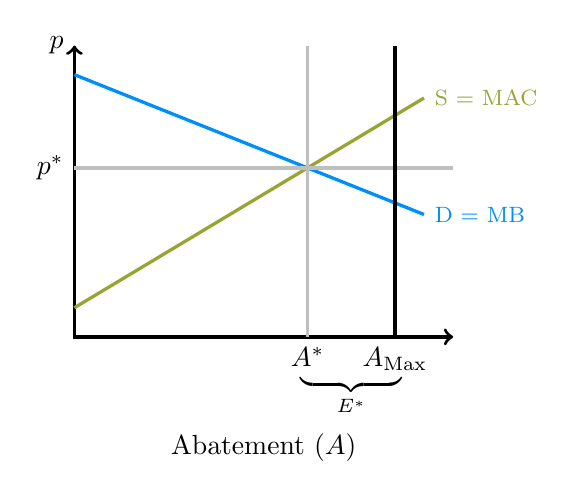
\begin{tikzpicture}[scale=0.37]
	\draw[very thick, <->] (0,10) node[left]{$p$} -- (0,0) -- (13,0); 	
	\draw[very thick, color2, domain=0:12] plot(\x, {.6*\x + 1}) node[right]{\footnotesize S = MAC};
	\draw[very thick, color1, domain=0:12] plot(\x, {-.4*\x + 9}) node[right]{\footnotesize D = MB}; 
	\draw[very thick, lightgray] (8,0) node[below, black]{$A^*$} -- (8,10);
	\draw[very thick, lightgray] (0,5.8) node[left, black]{$p^*$} -- (13,5.8);
	\draw[very thick] (11, 0) node[below]{$A_\text{Max}$} -- (11, 10);  
	\node[below] at (6.5, -3) {Abatement ($A$)};
	\draw (9.5, -2) node{$\underbrace{~~~~~~~~~~~}_{E^*}$};
\end{tikzpicture}
}
\hspace{.01cm}
\subcaptionbox{The Market for Emissions \label{emissions1}}{
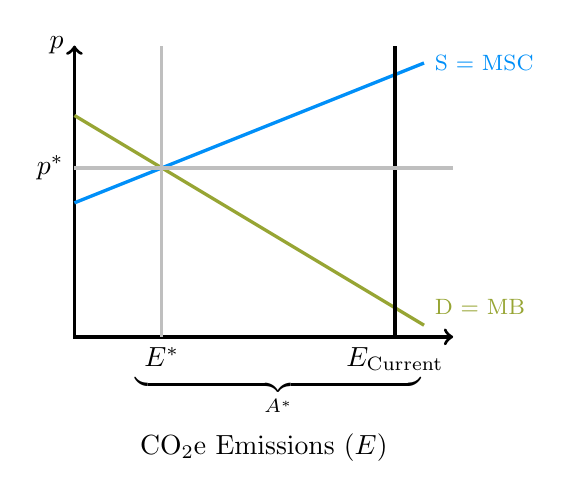
\begin{tikzpicture}[scale=0.37]
	\draw[very thick, <->] (0,10) node[left]{$p$} -- (0,0) -- (13,0);	
	\draw[very thick, color2, domain=0:12] plot(\x, {7.6 - .6*\x}) node[above right]{\footnotesize D = MB};
	\draw[very thick, color1, domain=0:12] plot(\x, {4.6 + .4*\x}) node[right]{\footnotesize S = MSC};
	\draw[very thick] (11, 0) node[below]{$E_\text{Current}$} -- (11, 10);
	\draw[very thick, lightgray] (3,0) node[below, black]{$E^*$} -- (3,10);
	\draw[very thick, lightgray] (0,5.8) node[left, black]{$p^*$} -- (13,5.8);	
	\node[below] at (6.5, -3) {CO$_2$e Emissions ($E$)};
	\draw (7, -2) node{$\underbrace{~~~~~~~~~~~~~~~~~~~~~~~~~~~~~~~}_{A^*}$};
\end{tikzpicture}
}
\vspace*{1em}
\fignote[1]{
	Figure presents two equivalent markets: (a) the market for abatement, and (b) the market for emissions. In the market for abatement D = MB is the demand for abatement or the marginal benefit of abatement, where the marginal benefit of abatement is equal to the marginal value of avoided damages; S = MAC is the supply of abatement or the marginal abatement cost; $A_\text{Max}$ is the maximum level of abatement, equal to the current level of emissions; $A^*$ is the equilibrium value of abatement; and $p^*$ is the price of abatement. In the market for emissions D = MB is the demand for emissions or the marginal benefit of emissions, where the marginal benefit of emissions is equal to the marginal value of avoided abatement; S = MSC is the supply of emissions or the marginal social cost of emissions; $E_\text{Current}$ is the current level of emissions; $E^*$ is the equilibrium level of emissions; and $p^*$ is the equilibrium price of emissions. The market for abatement and the market for emissions correspond such that the price of abatement and the price of emissions are the same, $A_\text{Max} - A^* = E^*$, and $E_\text{Current} - E^* = A^*$. Horizontal gray lines illustrate a hypothetical carbon tax and vertical gray lines illustration a hypothetical emissions cap.
}
\end{figure}

The previous example framed market-based instruments from the perspective of creating a market for emissions abatement, an approach that highlights how government intervention can work to establish a market for a public good. Although this framing is important and one that is often more convenient, the interpretation and public policy implications can seem counterintuitive. With government on the demand side, this would imply a policy where government pays polluters to abate, either promising a fixed rebate on each tonne of emissions abated or by purchasing abatement until it reaches $A^*$. In this system, polluters would earn more revenue through abatement. Major climate policy proposals do not include such massive payoffs to polluters, and rightly so; in the long run these economic profits would attract more firms to enter high-polluting industries and diminish the efficacy of the policy. There may also be additional social costs if the government reduces other expenditures or raises taxes in order to finance these payouts. 

The familiar policies focus on the inverse of the abatement market, the market for emissions. This market appears in Figure \ref{emissions1}. In this market, the government does not intervene to demand a public good, but to establish rights for and supply a public bad. The polluters derive their demand for emissions from their MAC curves, representing the most polluters will be willing to pay for the right to send CO$_2$e emissions into the atmosphere rather than abate. The supply curve in this market is the marginal damage of emissions. This framing comes with a clearer interpretation. Here, policymakers impose a carbon tax---a charge of $p^*$ on each tonne of CO$_2$e emissions. In equilibrium, this tax will lead to total emissions $E^*$. A cap-and-trade program instead sets a vertical supply curve of emissions allowances that give polluters the right to emit one tonne of CO$_2$e, at $E^*$. A key feature of these allowances is that they are tradeable between polluters. Although it is not necessary for government to sell or auction off emissions allowances, if government did, their equilibrium price would be $p^*$. 

Figure \ref{c_pricing} illustrates that the market for abatement and the market for emissions correspond. The difference between the maximum level of abatement and the equilibrium level of abatement is the equilibrium emissions, and the difference between the current level of emissions and the equilibrium level of emissions is the equilibrium abatement. The market price for emissions is the same as the market price for abatement. Framing market-based policy through the market for emissions has a more convenient interpretation relative to standard policy. However, because the prices and quantities are identical in both markets, economists often choose to frame market-based polices through the market for abatement rather than the market for emissions. This approach can be clearer when considering the cost-minimizing nature of market-based instruments.

The market for emissions also illustrates the equivalence of carbon pricing and a cap-and-trade program \emph{when the market is in equilibrium}. Every price on emissions corresponds with a single emissions cap, and every emissions cap corresponds with a single price on emissions. In this sense, a carbon tax and a cap-and-trade program are equivalent. Of course over time the marginal benefits curve will shift, and when this happens, the original supply curve set by the policy will no longer maximize welfare in the market for emissions.\footnote{The marginal social cost curve will also shift overtime, but will do so in more predictable ways.} When this occurs, then a carbon price and cap-and-trade program are no longer equivalent. In simplistic models of an emissions market like in Figure \ref{emissions1}, the elasticity of the emissions demand curve is useful for determining whether a carbon tax or an emissions cap is preferable. If the emissions demand curve is relatively elastic, then a carbon tax will make the market for emissions less volatile. If instead the emissions demand curve is relatively inelastic, then an emissions cap will make the market for emissions less volatile.

\begin{figure}
\caption{Distribution of Allowances with Carbon Pricing\label{dist_allowance}}
\centering
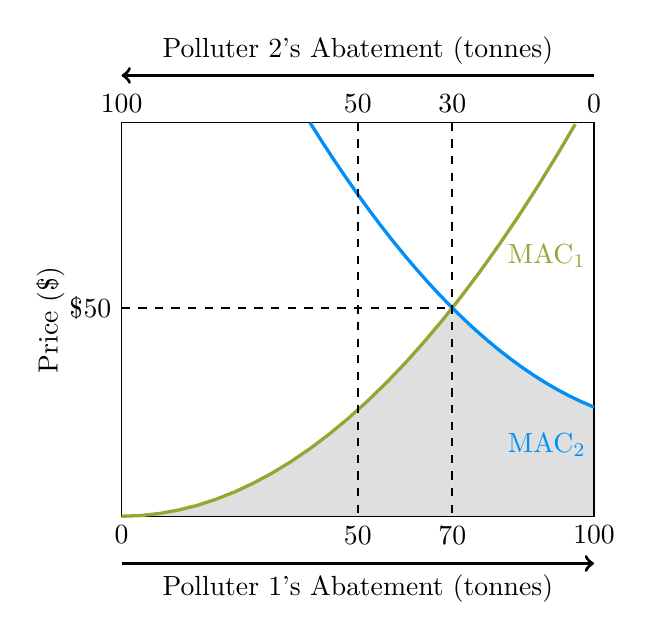
\begin{tikzpicture}[scale=0.6]
	\fill[lightgray!50!, domain = 0:7, variable = \x] (0,0) -- plot(\x, {.09*\x^2}) -- (7,0) -- cycle;
	\fill[lightgray!50!, domain = 7:10, variable = \x] (7,0) -- plot(\x, {.1*(12-\x)^2 + 1.91}) -- (10,0) -- cycle;
	\draw (0,0) rectangle (10,8.33);
	\draw (0,0) node[below]{0} -- (10,0) node[below]{100} -- (10,8.33) node[above]{0} -- (0,8.33) node[above]{100} -- (0,0);
	\draw[very thick, ->] (10, 9.33) -- (0, 9.33) node[pos=.5, above]{Polluter 2's Abatement (tonnes)};
	\draw[very thick, ->] (0, -1) -- (10, -1) node[pos=.5, below]{Polluter 1's Abatement (tonnes)};
	\draw[very thick, color2, domain=0:9.603] plot(\x, {.09*\x^2});
	\draw[very thick, color1, domain=3.988:10] plot(\x, {.1*(12-\x)^2 + 1.91}); 
	\draw[thick, dashed] (0,4.41) node[left]{\$50} -- (7,4.41);
	\draw[thick, dashed] (7,8.33) node[above]{30} -- (7,0) node[below]{70};
	\draw[thick, dashed] (5,8.33) node[above]{50} -- (5,0) node[below]{50};
	\node[rotate=90, above] at (-1, 4.155) {Price (\$)};
	\node[color2] at (9, 5.5) {MAC$_1$};
	\node[color1] at (9, 1.5) {MAC$_2$};
	% \draw[lightgray, thick] (5,0) node[below, black]{50} -- (5,8.33) node[above, black]{50};
\end{tikzpicture}
\fignote[1]{The figure visualizes the abatement market for Polluter 1 and Polluter 2. Polluter 1's abatement increases along the bottom horizontal axis, and Polluter 2's abatement decreases along the top horizontal axis. This arrangement means that at any point along the horizontal axis, the total abatement between the two polluters will be 100 tonnes. MAC$_1$ and MAC$_2$ represent the marginal abatement cost curves of Polluters 1 and 2 respectively.The shaded areas under the marginal abatement cost curves represent the total cost of abatement.}
\end{figure}

\begin{figure}[!htbp]
	\caption{Distribution of Allowances with Command-and-Control Policy\label{allowance_cost}}
	\centering
	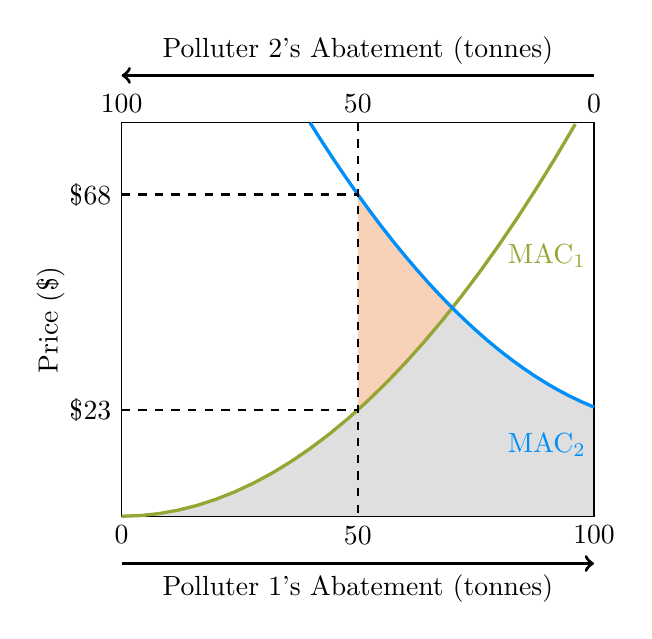
\begin{tikzpicture}[scale=0.6]
		\fill[lightgray!50!, domain = 0:5, variable = \x] (0,0) -- plot(\x, {.09*\x^2}) -- (5,0) -- cycle;
		\fill[lightgray!50!, domain = 5:10, variable = \x] (5,0) -- plot(\x, {.1*(12-\x)^2 + 1.91}) -- (10,0) -- cycle;
		\fill[color3!30!, domain=5:7, variable = \x] (5,4.3) -- plot(\x, {.1*(12-\x)^2 + 1.91}) -- (7,4.41) -- cycle;
		\fill[color3!30!, domain=5:7, variable = \x] (5,4.5) -- plot(\x, {.09*\x^2}) -- (7,4.41) -- cycle;
		\draw (0,0) rectangle (10,8.33);
		\draw (0,0) node[below]{0} -- (10,0) node[below]{100} -- (10,8.33) node[above]{0} -- (0,8.33) node[above]{100} -- (0,0);
		\draw[very thick, ->] (10, 9.33) -- (0, 9.33) node[pos=.5, above]{Polluter 2's Abatement (tonnes)};
		\draw[very thick, ->] (0, -1) -- (10, -1) node[pos=.5, below]{Polluter 1's Abatement (tonnes)};
		\draw[very thick, color2, domain=0:9.603] plot(\x, {.09*\x^2});
		\draw[very thick, color1, domain=3.988:10] plot(\x, {.1*(12-\x)^2 + 1.91}); 
		\draw[thick, dashed] (0,6.81) node[left]{\$68} -- (5,6.81);
		\draw[thick, dashed] (0,2.25) node[left]{\$23} -- (5,2.25);
		\draw[thick, dashed] (5,8.33) node[above]{50} -- (5,0) node[below]{50};
		\node[rotate=90, above] at (-1, 4.155) {Price (\$)};
		\node[color2] at (9, 5.5) {MAC$_1$};
		\node[color1] at (9, 1.5) {MAC$_2$};
		% \draw[lightgray, thick] (5,0) node[below, black]{50} -- (5,8.33) node[above, black]{50};
	\end{tikzpicture}
	\fignote[1]{The figure visualizes the abatement market for Polluter 1 and Polluter 2. Polluter 1's abatement increases along the bottom horizontal axis, and Polluter 2's abatement decreases along the top horizontal axis. This arrangement means that at any point along the horizontal axis, the total abatement between the two polluters will be 100 tonnes. MAC$_1$ and MAC$_2$ represent the marginal abatement cost curves of Polluters 1 and 2 respectively. The dotted vertical line represents a potential state allocation of abatement under a command-and-control policy. The shaded areas under the marginal abatement cost curves represent the total cost of abatement. Here, the yellow area represents the welfare loss incurred from the command-and-control policy.}
\end{figure}

Cap-and-trade programs come with the added complexity of determining how to initially distribute emissions allowances. It turns out that in our simple theoretical model of a cap-and-trade program with tradeable allowances, the initial distribution of allowances is irrelevant to whether or not the policy achieves the emissions reduction cost-effectively. Suppose that there are just two polluters in our system, Polluter 1 and Polluter 2, each of whom currently has 100 tonnes of emissions. The assumed benevolent policymaker wants to cut emissions in half by setting a cap of 100 tonnes of emissions between the two polluters. Polluter 1 and 2 have marginal cost of abatement curves depicted in Figure \ref{dist_allowance}. Consider two alternative scenarios: (1) the policymaker sells allowances to the polluters, and (2) the policymaker gifts 50 (tradeable) allowances to each polluter. 

If the policymaker sells allowances to the polluters, then both polluters will purchase allowances up until the price of an allowance equals the cost of an additional tonne of abatement. That is, each polluter will purchase the quantity of emissions allowances where the price of an allowance is equal to its marginal abatement cost. The demand for abatement is perfectly inelastic, so the equilibrium price will be where the sum of the quantities of abatement supplied by the polluters is 100 tonnes. Graphically, the total marginal abatement cost curve for the two polluters together is a horizontal summation of each individual marginal abatement cost curve. Figure \ref{dist_allowance} shows that at a price of \$50, the sum of Polluter 1 and 2's abatement is 100 tonnes, the desired level of abatement. Total abatement costs are equal to the area under each abatement curve from 0 to its level of abatement. 

Suppose instead each polluter begins with 50 allowances. If both have 50 allowances, Polluter 2 would have a far higher marginal cost of abatement than Polluter 1. Knowing this, Polluter 1 might sell some of its allowances to Polluter 2. Polluter 1 will sell its allowances as long as the price it receives is at least as high as its marginal abatement cost. Polluter 2 will buy allowances as long as the price it pays is weakly less than its marginal abatement cost. These dynamics bring the market to equilibrium where Polluter 1 sells 20 of its allowances to Polluter 2 at a price of \$50 per allowance. As before, this allocation of emissions and abatement minimizes total abatement costs. This shows that even if the two allowances are distributed uniformly and freely to polluters with heterogeneous marginal abatement costs, we still reach the cost-minimizing allocation of emissions abatement.

The major difference is not in the total costs, but in the distribution of these costs. If the policymaker uses an auction to allocate the allowances, then Polluter 1 will pay less (total) than Polluter 2, but both will bear the cost of purchasing emissions allowances and abatement costs; the cost of these allowances becomes government revenue. If the policymaker uniformly distributes the allowances between polluters, then Polluter 1 will collect additional revenues from selling 20 allowances, Polluter 2 will bear additional costs from buying another 20 allowances, and both bear their abatement costs. 

Although the optimal distribution of allowances is highly normative, conventional economic thought suggests that the auction method may have a slight welfare advantage over the gifting of allowances. Selling the emissions rights is considered \emph{non-distortionary}, as it corrects an existing market failure. If government used this additional revenue to reduce distortionary taxes, then this could lead to welfare gains in other pieces of the economy.

Before moving to a discussion of carbon pricing in practice, we revisit the earlier claim about market-based policies allocating abatement at the lowest cost. In Figure \ref{dist_allowance}, the gray shaded area under the curve represents the total cost of abatement between the two polluters. If market-based policies truly allocate abatement at the lowest cost, then this gray area must be the smallest the area under the two curves can be made. For comparison, consider a command-and-control policy where the state requires both polluters to abate their emissions by 50 tonnes. Figure \ref{allowance_cost} visualizes this scenario. Now the polluters incur different abatement costs at the margin, such that at the margin, it will cost Polluter 1 \$23 per tonne and Polluter 2 \$68 per tonne. Again, the shaded region under both curves represents the total cost of abatement. Recall that the costs represented by the area shaded in gray though were incurred under the emissions cap, but the costs represented by the area shaded in yellow were not. This yellow shaded area represents an unnecessary cost; the equivalent level of abatement is attainable without these costs. 

These additional costs from the command-and-control illustrate why economists are often distrustful of command-and-control policies. Notice that this lost welfare is dependent on where the state originally allocated abatement. When the state allocates abatement further from the market equilibrium (Polluter 1 abates 70 tonnes and Polluter 2 abates 30 tonnes), then this lost increases. When the state allocates abatement closer to the market equilibrium, then this lost decreases. Only in the case where the state allocates abatement exactly how the market allocates it will the welfare loss from the a command-and-control policy disappear. This demonstrates how carbon pricing tends to minimize costs more so than command-and-control policies.


\subsubsection{Carbon Pricing in Practice}

Conventional economic theory suggests that carbon pricing is the most  cost-effective option for emissions abatement. While the simple models discussed earlier in this section embody many of the ideas at the core of emissions pricing, these models also lack much of the nuance involved in the practical implementation of carbon pricing. We turn now to focus on carbon pricing policies in practice. 

Before delving too far into an empirical review of carbon pricing, it is worth considering whether or not carbon pricing is even worth discussing in the US. Even though it seems unlikely that the US would implement a nationwide carbon pricing program anytime in the relevant future, this has not always been the case. The Clean Air Act amendments of 1990---legislation championed by then President George H.W. Bush---established a nationwide cap-and-trade program on sulfur dioxide emissions through the Acid Rain Program. The broad bipartisan support of the legislation and overall success of the Acid Rain Program is at a minimum suggestive that similar policy for greenhouse gases might have at one time been politically feasible. The prospects for such a policy became palpable when the US House of Representatives passed the American Clean Energy and Security Act of 2009, more commonly known as the Waxman-Markey bill. The Waxman-Markey bill would establish a nationwide cap-and-trade program for greenhouse gas emissions highly analogous to the Acid Rain Program's cap-and-trade program on sulfur dioxide emissions. \cite{meng2017using} reviews data from the online trading exchange Intrade, which ran a contract allowing investors to, in essence,  bet on whether or not the Waxman-Markey bill would be signed into law and the US would have a nationwide cap-and-trade program for greenhouse gas emissions. These data suggest that at one point investors perceived the probability that the US would adopt a cap-and-trade program on greenhouse gases by the end of 2010 at 55\%. Ultimately the bill failed in the Senate, gaining some support from Republicans, but never enough to overcome the filibuster. It remains the only legislation that would price greenhouse gas emissions to pass a chamber of Congress. 

Today, a nationwide cap-and-trade program for greenhouse gas emissions in the US is generally understood to be politically infeasible. Still, several state and city governments across the country have taken up these policies as a part of their decarbonization strategy. Figure \ref{cap_states} displays the states with some form of carbon pricing. Currently, there at are thirteen states with carbon pricing programs, the most recent being Washington state which began its cap-and-trade program at the beginning of 2023. These states are among some of the most populous in the country, and the nearly a third (32.4\%) of the US population lives in a state with some form of carbon pricing. 

\begin{figure}
    \centering
    \caption{Statewide Carbon Pricing in the US\label{cap_states}}
    \includegraphics[width = \textwidth]{figures/chapter3_figures/cap_programs.pdf}
    \vspace*{-1.8cm}
    \fignote[1]{
        Figure displays statewide carbon pricing policies as of January 1, 2023 for the contiguous 48 states. Economy-wide cap-and-trade programs price emission from electricity, as well as other sectors, like industrial processes and transportation fuel distributors. Electricity-only cap-and-trade programs only pricing emissions from the electric power industry. Together, there are thritheen states with carbon tax or cap-and-trade programs at the state level in the US. The remaining 37 states do not have carbon pricing programs. Records from \cite{c2es_map}.
    }
\end{figure}

However, as Figure \ref{cap_states} shows, most of these states have programs that only cover emissions from electric power generation. These states on the East Coast all belong to the Regional Greenhouse Gas Initiative, an emissions trading scheme that applies only to fossil fuel powerplants in participating states. The cap-and-trade programs in California, Washington, and Quebec are all connected through the Western Climate Initiative, another market where participants can purchase emissions allowances. Unlike programs on the East coast, California and Washington's programs cover emissions outside of electricity, including some industrial emissions and transportation-related emissions. 

Outside of the US, carbon pricing is among the most popular decarbonization policies. The European Union has operated its own cap-and-trade program known as the Emissions Trading System (EU ETS) since 2005. The cap covers about 40\% of all greenhouse gas emissions in the EU primarily from electric power generation and other energy intensive industries \citep{eu_ets_overview}. Up until 2021, the EU ETS was the worlds largest carbon pricing system. In 2021, China began its own cap-and-trade program. Currently, China's cap-and-trade program covers only emissions from its electric power sector, but these emissions are substantial. The cap-and-trade system covers about 4.5 billion tonnes of CO$_2$ annually, twice the volume of emissions covered under the EU ETS. For comparison, the US totals around 5 billion tonnes of CO$_2$ annually. The Chinese government has stated that it plans to phase additional industries into the carbon pricing program as a part of its goal to peak emissions by 2030 and go carbon neutral by 2060 \citep{icap_report}. Globally, there are 70 carbon pricing initiatives (including national and subnational programs) which covered about 23\% of all CO$_2$e emissions in 2022 \citep{wbank}. 

Clearly carbon pricing is fairly popular among economists and policymakers around the world, but this does not reveal whether or not carbon pricing actually works. In general, it is difficult to assess the efficacy of carbon pricing programs ex-post. These programs usually are phased in slowly to ensure a smooth transition, a design that makes identifying the effect of these policies difficult because there are no sudden shocks that make for easy comparison of emissions pre- and post-implementation. Additionally, these programs are rarely if ever implemented in isolation. For instance, California's emissions trading program was first implemented alongside its clean energy portfolio standard. Again, this makes for a difficult comparison because we cannot easily identify what effects are attributable to the carbon pricing program and what effects are attributable to the other climate policies. Lastly, there is the trouble with the actual price of emissions. Even if researchers can overcome these other challenges and can identify the causal effect of a carbon pricing program on emissions, this will not have a clear implication for the emissions price. For instance, if the causal effect of a carbon pricing program on emissions is relatively small, then its not clear if the lack of efficacy is due to a flaw in the policy design or due to a price on emissions that is simply too low. Despite the challenges involved in evaluating the efficacy of carbon pricing programs, there is still plenty of room to glean insight on these programs. The remainder of this section overviews five key conclusions related to the function and success of carbon pricing. 

First, there is a desperate need for research that can offer an ex-post analysis of carbon pricing programs. Billions of dollars in allowances are already traded every year on emissions markets, yet credible ex-post analyses on the efficacy of these programs are scarce. This is no small task, and given the complexity of identification, this may only be possible if researchers collaborate with policymakers to implement policies in ways that will allow for strong ex-post analysis. \cite{green2021does} offers a timely meta-analysis of the existing literature on the effect of carbon pricing on emissions abatement. In her meta-analysis, Green finds just 37 papers from peer-reviewed journals, working papers series, and non-government entities that measure the effect of carbon pricing on emissions abatement. Most of these rely on dubious identification strategies, particularly matching on observables, which could potentially suffer substantially from omitted variable bias, and difference-in-differences, which has trouble with the many layered nature of treatments as well as dealing with the magnitude (price) of the treatment. Still, the meta-analysis suggests that often carbon pricing programs only result in emissions reductions between 0\% and 2\% annually, a finding that Green summarizes by stating ``[overall], the evidence indicates that carbon pricing has a limited impact on emissions.''

This apparent criticism motivates the second key takeaway: there is evidence that many of the jurisdictions that have already implemented carbon pricing programs rely extensively on other regulations to induce the majority of abatement. Given the lackluster performance of carbon pricing presented in \cite{green2021does}, this consideration is valuable for assessing the potential of carbon pricing in the future. Simply acknowledging that traditional regulations are currently creating more abatement does not represent a failure of carbon pricing, but instead reflects the preferences of policymakers. To see more impressive results from carbon pricing, the price of carbon must increase faster than the shadow price of other climate regulation.

\begin{figure}
	\centering
	\caption{Emissions Trading in Practice \label{c_pricing_prac}}
	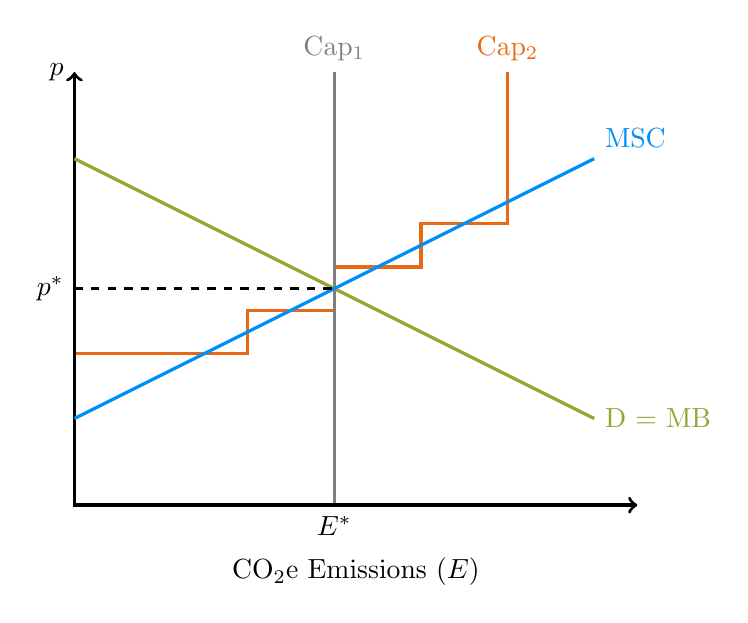
\begin{tikzpicture}[scale=0.55]
		\draw[very thick, color3] (0, 3.5) -- (4, 3.5) -- (4, 4.5) -- (6, 4.5) -- (6, 5.5) -- (8, 5.5) -- (8, 6.5) -- (10, 6.5) -- (10, 10) node[above]{Cap$_2$};
		%\draw[very thick, color3] (0, 2.5) -- (8, 2.5) -- (8, 3.5) -- (10, 3.5) -- (10, 4.5) -- (12, 4.5); 
		\draw[very thick, gray] (6,0) node[below, black]{$E^*$} -- (6,10) node[above]{Cap$_1$};
		\draw[very thick, <->] (0,10) node[left]{$p$} -- (0,0) -- (13,0);	
		\draw[very thick, color2, domain=0:12] plot(\x, {8 - .5*\x}) node[right]{D = MB};
		\draw[very thick, color1, domain=0:12] plot(\x, {2 + .5*\x}) node[above right]{MSC};
		% \draw[very thick] (11, 0) node[below]{$E_\text{Current}$} -- (11, 10);
		\draw[very thick, dashed] (0,5) node[left, black]{$p^*$} -- (6,5);
		\node[below] at (6.5, -1) {CO$_2$e Emissions ($E$)};
	\end{tikzpicture}
	\fignote[1]{
		Figure displays the market for emissions under two different types of emissions ``caps.'' In this market, D = MB is the demand for emissions, MSC is the marginal social cost of emissions, $p^*$ is the equilibrium price of emissions, and $E^*$ is the equilibrium level of emissions. There are two potential caps in this market. Cap$_1$ illustrates the standard notion of a cap on emissions---a fixed quantity of emissions. Cap$_2$ illustrates a more realistic notion of the cap on emissions. With this ``cap,'' price increases can trigger the release of additional allowances, and price decreases can trigger cuts in the number of allowances available. 
	}
\end{figure}

To establish why policy analysts understand that in many jurisdictions complementary programs are responsible for the majority of emissions reductions, consider California's emissions trading program. California's emissions trading program differs in a few key ways from the traditional notion of a cap-and-trade program presented in Figure \ref{c_pricing}---as do most emissions trading programs. As it is typically imagined, the cap in a cap-and-trade program is a vertical supply curve for emissions allowances. This idea of an emissions cap appears as Cap$_1$ in Figure \ref{c_pricing_prac}. When the demand for emissions shifts, the price of allowances may change, but the quantity of emissions will not. In practice though emissions trading programs rarely have a set ``cap,'' hence why they are often called emissions trading programs rather than cap-and-trade programs. 

Instead, many emissions trading programs are structured as a hybrid between a carbon tax and a cap-and-trade program \citep{schmalensee2017lessons}. Cap$_2$ displays a more realistic supply curve for emissions allowance. Going left to right, there are three regions to this supply curve: (1) the absolute price floor, (2) the hybrid region, and (3) the absolute emissions cap. The absolute price floor is the lowest price the regulator will allow an allowance to sell at, like the starting price of an emissions allowance at auction. This portion of allowance supply curve behaves like a carbon tax in that polluters will pay a fixed price per tonne for their emissions. The absolute cap is the greatest number of allowances that the regulator will allow to go up for sale on the market. This portion of the allowance supply curve behaves like a traditional cap in that polluters cannot emit more than this set quantity. 
As \cite{schmalensee2017lessons} note, the hybrid region is composed of incremental emissions caps arranged like stairsteps or ``price collars.'' If the price of allowances increases enough above the absolute price floor, then this will trigger regulators to release additional emissions allowances. If the price of allowances increase above the minimum price at the previous step, this will again trigger regulators to release additional emissions allowances. This continues until the absolute emissions cap is reached, in which case higher allowance prices will not trigger the release of additional allowances.

The primary advantage of this design over of the standard cap-and-trade or carbon tax is reduced volatility. If the demand for allowances shifts, this design will result in a smaller change in price than a standard cap-and-trade program and a smaller change in emissions than a standard carbon tax. Providing this stability attracts investors and prevents firms from ``hoarding'' emissions allowances when they are cheap, in the hopes of using these permits later on when the cap becomes tighter. Now firms have some expectation that if there is a sudden spike in allowance prices, that regulators will release more permits to soften the blow. 

\begin{figure}
    \centering
    \caption{California Emissions Allowance Price \label{allowance_pr}}
    \includegraphics[width=\textwidth]{figures/chapter3_figures/allowance_prices.pdf}
    \fignote[1]{Figure displays the auction price and price floor for emissions allowances in California from Q4 2015 through Q4 2022. Each emissions allowance covers one tonne of CO$_2$e emissions. Data on emissions allowances come from the California Air Resources Board, \cite{carb_prices}.}
\end{figure}

For most emissions trading programs, the price of emissions allowances has remained near the absolute price floor for almost the entire history of the program. Figure \ref{allowance_pr} displays the price of California emissions allowances at auction alongside the price floor. Note first that regulators shift in the supply curve for emissions each year, a fact reflected in the annual increases in the absolute price floor. From most of the program's history, the auction price is just above the price floor. This took a turn in the first and second quarter of 2021, when prices spiked well above the price floor amidst the emergence of China's emissions market, a growing interest in holding emissions allowances as an asset, and anticipated tightening of the cap over the next decade \citep{storrow2022price}.\footnote{Allowance prices around the world substantially increased in 2021. This was particularly true in Europe, where the price per tonne of CO$_2$e briefly shot up to about \$100 per tonne before settling closer to \$80 per tonne \citep{manzagol2022global}. Under the Biden Administration, the social cost of carbon used in Federal studies is \$52 per tonne.} The price of carbon generally staying near the price floor is consistent with the suggestion that the existing cap is simply too high to create any substantial emissions reductions relative to other policies. 

There are of course alternative explanations for the proximity of allowance auction prices and the price floor. For instance, it could be that the price floor is just high relative to the shadow price of other regulations, in which case the price floor would be binding but the emissions trading program should be responsible for the majority emission reductions. If this were the case, then even high prices would not lead to abatement and we would have to conclude that carbon pricing is not effective in practice. In California though, policymakers have been clear that the reason allowance prices are near the absolute price floor is because emissions reductions are being led by other regulation. In an interview \citep{burtraw2022_rff}, Dallas Burtraw, the Chair of California's Independent Emissions Market Advisory Committee (IEMAC),\footnote{IEMAC is a group of researchers that advises the California Air Resources Board on how to manage its emissions trading program.} describes the policymaking process and the decisions that ensure this is the case:
\begin{quote}
	\singlespacing ``The primary way that emissions reductions have been achieved is \\through regulations and standards\ldots California has a process called the Scoping Plan process. It's a multiagency project, and they develop a blueprint for how the state's going to achieve its climate reduction goals. The first Scoping Plan identified over 80 percent of the emissions reductions that were needed to be achieved, associated with regulations, and only the remaining 20 percent (approximately) of emissions reductions were associated with the influence of the cap-and-trade program and the price of emissions allowances. The next Scoping Plans increase that share that was associated with the price effect of the cap-and-trade program up to the neighborhood of 40 percent.''
\end{quote}
This leads to the conclusion that if emission reductions from carbon pricing seem modest (as \cite{green2021does} suggests), it is because the price of emissions is just relatively low, not because the program is ineffective. Burtraw also indicates that California's cap-and-trade program is designed to take on a larger role in emissions reductions during the next phase of the state's climate strategy.

The third primary takeaway is the acknowledgement that current carbon pricing policies have room for improvement. For over a decade, policy scholars have understood two primary issues with carbon pricing: emissions leakage and carbon offsets \citep{cullenward2014carbon}. The next section considers emissions leakage in greater detail, but as a preview, emissions leakage may mean that carbon pricing just moves emissions into jurisdictions that do not have such stringent climate policy. It is possible in some scenarios that there could be a substantial volume of emissions that ``leak'' into other jurisdictions. It is also possible that certain strategies to prevent leakage might undermine the efficacy of the carbon price, namely the practice of distributing free allowances to select industries. Although this is an issue with carbon pricing, it is an also issue that arises with command-and-control climate policy. This means that if the counterfactual in mind is an alternative policy, emissions leakage is not a valid critique of carbon pricing.

Carbon offsets on the other hand are an issue unique to emissions trading programs. The idea of a carbon offset is straightforward; to lower their net emissions, polluters can pay for emissions sequestration or emissions abatement elsewhere rather than abate their own emissions. For instance, abatement options in the aviation industry are limited primarily to fuel switching, which has difficulty eliminating a majority of CO$_2$e emissions even with substantial investment in alternative fuels \citep{dray2022cost}. Instead, airline operators could reduce their net emissions by planting trees or by paying others to abate their emissions (i.e., an emissions allowance that is not confined to the regulated jurisdiction). Provided they truly represent emissions reductions, carbon offsets provide a strategy to reduce net emissions in the face of emissions that are difficult to abate.

The issue with carbon offsets is that they often do not represent real emissions reductions. As an example, \cite{west2020overstated} study carbon offsets generated by Reduced Emissions for Deforestation and Forest Degradation (REDD$+$) zones in the Brazilian Amazon. Carbon offsets for this program---established by the United Nations Framework Convention on Climate Change---are generated by saving forest that would otherwise be destroyed and unable to sequester greenhouse gas emissions. The trouble is of course getting an accurate measurement of the emissions reductions that this reduced deforestation creates. If companies were already planning on not clearing this land, then there is not really any emissions reduction. \cite{west2020overstated} use synthetic controls to establish the relevant counterfactual and do not find any significant evidence that REDD$+$ programs have actually mitigated deforestation. The researchers results suggest that of the 5.4 million tonnes of carbon offset credits certified, only about 30,000 tonnes of credits (0.56\%) are legitimate. 

Carbon offsets are widely understood by even non-researchers to be less effective than they appear, but not entirely ineffective \citep[see, for example,][]{astor2022airline}. As a result, emissions trading programs that accept carbon offsets are likely less effective than they appear as well. Still, there are legitimate efforts both to (1) make carbon offsets more credible, and (2) limit the use of carbon offsets in emissions trading. To the first point, California has attempted to improve the credibility of carbon offsets by limiting carbon offset credits to a list of projects that the state can verify \citep{carb_offsets}. To the second point, California limits the use of carbon offsets to 4\% of an entity's emissions obligation \citep{carb_offsets_about}. Carbon offsets are still a weak point for emissions trading programs, but a weak point that is increasing small in scope. 

Fourth, there is little reason to believe that carbon pricing is not effective. The previous takeaways have made clear that if carbon pricing programs appear ineffective relative to other emissions reduction programs, this is likely because the regulators have largely used carbon pricing in only a complementary role. Additionally, while carbon pricing programs are not perfect, the most significant issues are still small in scope. As a result, there is just not substantial, credible evidence that carbon pricing will not be effective at reducing emissions as regulators begin to prioritize these programs in the decarbonization planning. Other emissions trading programs for criteria air pollutants in the US have been highly successful \citep{schmalensee2017lessons}. Importantly, compliance rates for carbon pricing programs are extremely high; year after year, 100\% of businesses meet all their emissions obligations in California \citep{carb_comp_2018, carb_comp_2021}. Assuming the high rates of compliance continue, raising the carbon tax or reducing the cap must imply the corresponding level of emissions abatement. Carbon pricing can successfully reduce greenhouse gas emissions.

Of course the primary argument for the use of carbon pricing is not that it can reduce greenhouse gas emissions. After all, there are a variety of other policies that can also achieve emissions reductions. The primary argument for the use of carbon pricing is that it is cost-effective, a point that leads to the fifth and final takeaway on carbon pricing: in some contexts, there is also little reason to believe that carbon pricing is substantially more cost-effective than some command-and-control policies. \cite{borenstein2022carbon} provide good reason to believe that for the electric power industry, clean energy standards may come with a price tag comparable to a carbon tax. The explanation behind this is that there is a strong positive correlation between the social costs and private costs for ``dirty'' generation. A clean energy standard (CES) is a command-and-control policy that sets a minimum proportion of electricity in the state that must come from sources designated as ``clean''. Equivalently, a CES sets a maximum proportion of electricity that can come from ``dirty'' sources. Because a CES does not differentiate between generation within the ``dirty'' group, standard theory would predict that a CES will be inefficient---a coal plant might outlive a natural gas plant despite being far dirtier. However, within those power plants designated as ``dirty'' those are dirtier also tend to have higher marginal costs. This translates into an allocation of generation under a CES that is similar to the allocation of generation under a carbon price. Clean energy subsidies---which are usually thought to be even more inefficient, as they make electricity cheaper and thereby increase the quantity demanded of an emissions intensive good---may be efficient as well. Here the key is that retail electricity prices are already well above the socially optimal price, meaning that command-and-control subsidies may reduce emissions while moving prices in a socially optimal direction. 

The upshot of this is whether or not this result from the electric power industry generalizes to other industries as well. This question is more difficult because less is known about the private costs these firms face. Intuition suggests that this does not hold as well in other industries. Retail electricity prices well-above the socially optimal prices is a result of the unique pricing structure of electricity and there is little reason to believe this would be true of other emissions intensive industries like cement production. There is likely a correlation between social costs and private costs in other industries that stems from energy efficiency, but this correlation is also likely to be looser as these other industries will be less energy intensive than electric power generation. Overall, context is important when considering the cost savings that a carbon price offers over command-and-control regulations. 

% Chapter 2 describes arguments against carbon pricing that critique the efficacy of these programs. This discussion comes to four primary conclusions. First, there is a need for additional research that measures the ex-post effect of carbon pricing on emissions reductions. Second, many jurisdictions with carbon pricing programs have chosen to rely on other regulations to attain emissions targets. That is, the implicit price on emissions from other regulations is often higher than the market price of emissions, which can make the effect of emissions pricing appear weak relative to other regulations. Third, in situations where policymakers rely primarily on carbon pricing more so than other regulations, carbon pricing does appear to be the more cost-effective policy. This difference appears to be small though, especially in the electricity market where the strong correlation between the merit order of generation and emissions intensity mean that clean energy standards perform only negligibly worse carbon pricing. Fourth, there are likely tangible improvements to emissions trading programs that can be made, such as reforming or eliminating the use of emissions offsets. 



\subsection{Unilateral Climate Policy \& Leakage}

% \begin{quote}
% 	``You know these pest control companies. They call themselves exterminators, but they can't really do it. The best they can do is get the bugs to go to somebody else's house. They just relocate them, you know what I mean? They're bug realtors is what they are."\\ \\[-1.8ex]
% 	--- Jerry Seinfeld on the follies of incomplete regulation (Seinfeld, Season 6, Episode 19, ``The Doodle")
% \end{quote}

The previous section looked at the ability of carbon pricing to reduce greenhouse gas emissions within a closed economy. Although this is the standard presentation of carbon pricing, in actuality, carbon pricing occurs for open economies. This distinction creates potentially difficulties for many policies aimed at curbing emissions, including carbon pricing. 

When an individual jurisdiction takes up a carbon pricing program, this is known as \emph{unilateral} carbon pricing, meaning that this jurisdiction adopts the policy without coordinated carbon pricing schemes across all or most all other jurisdictions in its same trade network. This is the current state of carbon pricing programs. Recall that 23\% of all CO$_2$e emissions face a carbon price, meaning that the majority of emissions do not face a carbon price \citep{wbank}. Unilateral carbon pricing is an example of an incomplete regulation: a situation where not all relevant actors in the market face regulation. In the case of greenhouse gas emissions, everyone is a relevant actor, meaning that without a global carbon pricing scheme, any unilateral carbon pricing scheme will always be incomplete. For example, even if Country A has a price on its carbon, it will not be able to put a price on the emissions from Country B, even though Country B's emissions are just as damaging to Country A as its own emissions. That is not to say that unilateral carbon pricing schemes are not worth it, but to acknowledge that the policy misses some emissions. 

The purpose of this section is to explore the impacts of incomplete climate policy on the efficacy of this policy. Most of the examples focus on carbon pricing, but many of the discussion generalizes to other climate policies that create asymmetric regulation within markets. This begins with a discussion of how climate policy affects the geographic distribution of economic activity, and then moves on to consider both the implications of this redistribution on net emissions and the strategies available to address the issue.

A frequent claim of those opposing aggressive climate policy is that it will make the domestic economy ``less competitive" than foreign economies. That is, some claim that foreign firms will gain a greater global market share as a result of higher domestic regulatory costs. Understandably, the effect of climate and environmental policy on domestic economic activity is of considerable interest to not just economists, but policymakers and the general public.

Central to the debate among researchers on the topic are two competing perspectives: the pollution haven hypothesis and the Porter Hypothesis \citep{dechezlepretre2020impacts}. The pollution haven hypothesis holds that increasing domestic environmental policy stringency will make domestic firms relatively less competitive than foreign firms, shifting economic activity towards foreign economies. This claim is familiar; if the US implemented a nationwide carbon tax, then production prices in the US would rise relative to foreign production prices, leading consumers both in the US and abroad to buy fewer US goods. The Porter hypothesis, popularized in \cite{porter1995toward}, holds instead that increasing domestic environmental policy stringency will make domestic firms relatively \emph{more} competitive than foreign firms, shifting economic activity towards the domestic economy. The argument is that increasingly stringent environmental regulation induces efficiency improvements and R\&D investment that will result in lower domestic production costs, and ultimately a shift in economic activity towards the domestic economy. For instance, if a climate policy switches electricity generation from fossil fuels to renewables, this could lower the retail price of electricity and lower the costs of domestic producers. 

Contemporary empirical evidence on the pollution haven and Porter hypotheses leads to a few key conclusions: (1) environmental regulation does not have an economically significant effect on aggregate trade flows, and (2) environmental regulation can have an economically significant effect on the trade flows of specific industries that is consistent with the pollution haven hypothesis. A common technique for assessing differences in climate policies is considering differences in energy prices \citep[see, for example,][]{fowlie2022mitigating}. The idea is that carbon prices function in the short run by raising the price of energy that a firm's technology relies on. Using differences in energy prices as a proxy, \cite{sato2015asymmetric} show that a 10\% increase in the energy price gap between trading countries only increases bilateral manufacturing trades by 0.2\%. Further these same energy price differences only explain 0.01\% of the variation in trade flows. \cite{aldy2015competitiveness} find a null result in a similar study looking at energy price differences between US states---the effect of energy price differences on total manufacturing imports between states was statistically insignificant, even with their over thirty years of panel data. However, they do find pronounced effects in certain, energy intensive sectors including steel, industrial chemicals, and cement. Similarly, in their survey of the literature, \cite{dechezlepretre2020impacts} come to the conclusion that there is likely a pollution haven effect, but that it is confined to a select number of industries.


The existence of a pollution haven effect is interesting in its own right, but the effect on the relative competitiveness of domestic and foreign firms does not immediately speak to the efficacy of climate policy. Taken a step further though, it is clear that if climate policy shifts economic activity towards the foreign, under-regulated jurisdictions, this will also imply that the greenhouse gas emissions created by this economic activity shift into foreign jurisdictions as well. Unfortunately, even if the transfer of economic activity is small overall, the transfer of emissions can be quite large.

This is a part of a broader process known as \emph{emissions leakage} that occurs when the implementation of a stringent regulation on greenhouse gas emissions in one place leads to increased greenhouse gas emissions in another place with looser regulations. Assuming the goal of climate policy is to mitigate climate damages by reducing global emissions, rather than just hitting a domestic emissions target, then emissions leakage could seriously undermine the efficacy of climate policy. 

% Emissions leakage is closely related to the pollution haven hypothesis, but differs in a few ways. First, emissions leakage refers exclusively to GHG emissions, not pollution in general. This distinction is important as most GHG emissions have a negligible effect on the areas downwind from their source of emissions, but ambient air pollutants do not. Thus, the consequences of increased GHGs from emissions leakage is global rather than local. Second, the pollution haven hypothesis is much more concerned with international trade flows and the changing composition of economies, whereas emissions leakage is concerned more with changing the distribution of emissions. That is, the pollution haven hypothesis focuses on the implications of displaced economic activity, and emissions leakage focuses on the implications of displaced emissions.

\begin{figure}[!htbp]
\caption{Competitive Emissions Leakage \label{leakage_ex}}
\centering
\singlespacing
\footnotesize
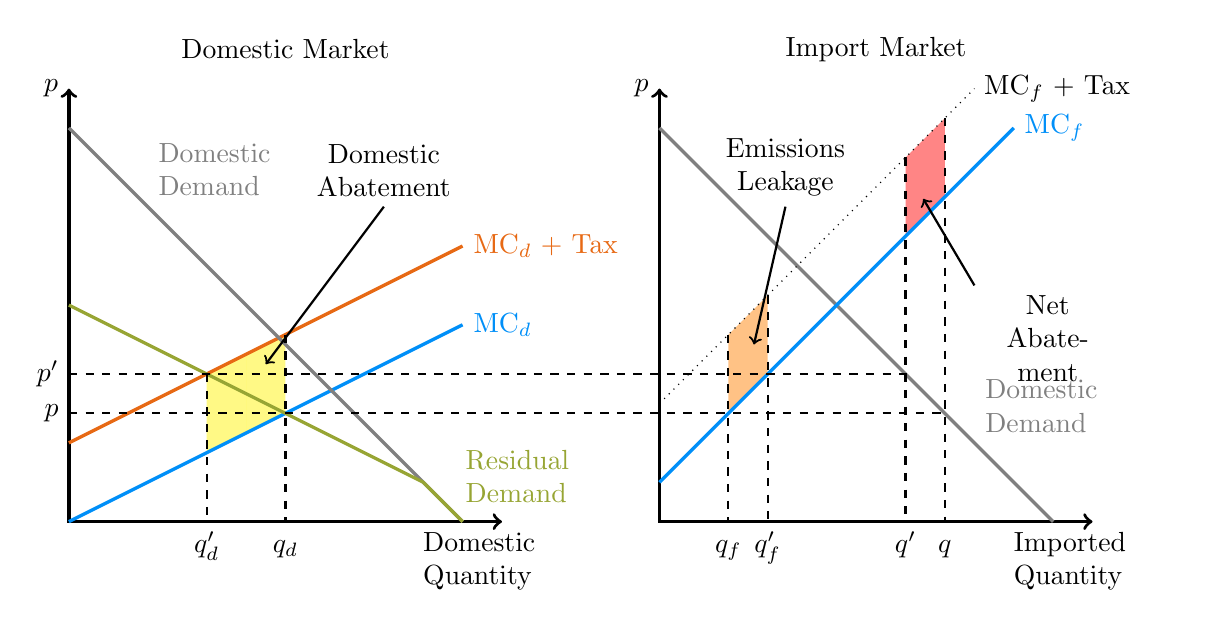
\begin{tikzpicture}[scale = 0.5]
	\draw[very thick, <->] (0, 11) node[left]{$p$} -- (0, 0) -- (11, 0) node[below, text width = 2cm]{Domestic Quantity};
	\draw[very thick, <->] (15, 11) node[left]{$p$} -- (15,0) -- (26, 0) node[below, text width = 2cm]{Imported Quantity};
	\fill[yellow!80!, opacity = 0.6] (3.5, 3.75) -- (3.5, 1.75) -- (4.5, 2.25) -- (4.5, 4.25) -- cycle;
	\fill[yellow!80!, opacity = 0.6] (4.5, 2.25) -- (5.5, 2.75) -- (5.5, 4.75) -- (4.5, 4.25) -- cycle;
	\fill[orange!80!, opacity = 0.6] (16.75, 4.75) -- (16.75, 2.75) -- (17.75, 3.75) -- (17.75, 5.75) -- cycle;
	%\fill[orange!80!, opacity = 0.6] (16.25, 4.25) -- (16.25, 2.25) -- (16.75, 2.75) -- (16.75, 4.75) -- cycle;
	\fill[red!80!, opacity = 0.6] (21.25, 9.25) -- (21.25, 7.25) -- (22.25, 8.25) -- (22.25, 10.25) -- cycle;
	%\fill[red!80!, opacity = 0.6] (20.75, 8.75) -- (20.75, 6.75) -- (21.25, 7.25) -- (21.25, 9.25) -- cycle;
	\draw[very thick, color1] (0,0) -- (10, 5) node[right]{MC$_d$};
	\draw[very thick, color3] (0,2) -- (10, 7) node[right]{MC$_d$ $+$ Tax};
	\draw[very thick, gray] (0, 10) -- (10,0) node[pos=.2, above right,text width = 1.5cm]{Domestic Demand}; 
	\draw[very thick, color2] (0,5.5) -- (9, 1) -- (10, 0) node[pos=.8, above right, text width = 1.5cm]{Residual Demand};
	%\draw[very thick, color2] (0, 6.5) -- (7,3) -- (10, 0);
	\draw[very thick, gray] (15, 10) -- (25, 0) node[pos=.8, above right,text width = 1.5cm]{Domestic Demand}; 
	\draw[very thick, color1] (15, 1) -- (24, 10) node[right, text width = 1.5cm]{MC$_f$};
	\draw[dashed, thick] (5.5, 4.75) -- (5.5, 0) node[below, yshift = -3pt]{$q_d$};
	\draw[dashed, thick] (3.5, 3.75) -- (3.5, 0) node[below]{$q_d'$};
	%\draw[dashed, thick] (4.5, 4.25) -- (4.5, 0) node[below]{$q_d''$};
	\draw[dashed, thick] (0, 3.75) node[left]{$p'$} -- (21.25, 3.75);
	\draw[dashed, thick] (0, 2.75) node[left]{$p$} -- (22.25, 2.75);
	%\draw[dashed, thick] (0,4.25) node[left]{$p''$} -- (20.75, 4.25);
	\draw[dashed, thick] (16.75,4.75) -- (16.75, 0) node[below, yshift = -3pt]{$q_f$};
	\draw[dashed, thick] (17.75, 5.75) -- (17.75, 0) node[below]{$q_f'$};
	%\draw[dashed, thick] (16.25, 4.25) -- (16.25, 0) node[below]{$q_f''$};
	\draw[dashed, thick] (22.25, 10.25) -- (22.25, 0) node[below, yshift = -3pt]{$q$};
	\draw[dashed, thick] (21.25, 9.25) -- (21.25, 0) node[below]{$q'$};
	%\draw[dashed, thick] (20.75, 8.75) -- (20.75, 0) node[below]{$q''$};
	\draw[dotted] (15, 3) -- (23, 11) node[right]{MC$_f$ $+$ Tax};
	\draw[thick, <-] (5, 4) -- (8, 8) node[above, text width = 2cm, align=center]{Domestic Abatement};
	\draw[thick, <-] (17.4, 4.5) -- (18.2, 8) node[above, text width = 2cm, align=center]{Emissions Leakage}; 
		\draw[thick, <-] (21.7, 8.2) -- (23, 6) node[below right, text width = 1.6cm, align=center]{Net Abatement};
		\node at (5.5, 12) {Domestic Market};
		\node at (20.5, 12) {Import Market}; 
\end{tikzpicture}
\vspace*{1em}
\fignote[1]{
	Figure adapted from Figure 2 in \cite{fowlie2016measuring} depicts the domestic market and import market for an EITE good. Residual demand in the domestic market is calculated as the difference between the quantity demanded and the quantity supplied in the import market. Subscripts of $d$ denote a domestic quantity ($q$) or marginal cost (MC), and $f$ denote a foreign quantity or marginal cost. Quantities and prices ($p$) with an $'$ are after the carbon tax has been applied, and quantities and prices without an $'$ are before the carbon tax has been applied. The yellow shaded region represents the value of domestic emissions reductions, the orange shaded region represents the cost of increases in foreign emissions (i.e., emissions leakage), and the red shaded region represents the value of the net emissions abatement.
}
\end{figure}

Figure \ref{leakage_ex} displays how competitive effects can drive emissions leakage in the market for an emissions-intensive good. In the left panel of Figure \ref{leakage_ex} is the domestic market for an arbitrary emissions-intensive good. In the right panel of Figure \ref{leakage_ex} is the import market for the same good. Domestic producers do not face the full domestic demand curve, as foreign producers will also be willing to supply the domestic market. Instead, domestic producers face the residual demand curve---the difference between the domestic quantity demanded and the import supply at each price. Domestic firms will produce where their marginal cost curve MC$_d$ intersects residual demand. This price then caries into the import market, and foreign firms will produce where the domestic market price intersects their marginal cost curve MC$_f$. Absent any carbon pricing scheme, domestic firms produce $q_d$, foreign firms import $q_f$, and the total market quantity is $q$. 

Now suppose that domestic policymakers implement a carbon pricing scheme. For ease, assume that this takes the form of a per tonne emissions tax and that marginal emissions and marginal damages from emissions are both constant. The carbon pricing scheme is unilateral, meaning that it applies to all domestic producers, but not any foreign producers. The constant marginal emissions rate and per unit carbon tax imply that domestic firms pay a constant per unit tax on their output, creating a parallel shift up in from MC$_d$ to MC$_d$ $+$ Tax. Again, firms produce where the marginal cost they face equals residual demand. This causes the domestic price of the good to rise to $p'$ and the domestic production of the good to fall to $q_d'$. The yellow region of left panel in figure \ref{leakage_ex} represents a monetary measure of domestic abatement. If the tax on emissions is set equal to the social cost of a tonne of emissions, then this area is the monetary value of all domestic emissions abatement, $\text{Tax} \times E \times (q_d' - q_d)$, where $E$ is the emissions intensity of the good measured in tonnes CO$_2$e per unit. Like we should expect, the carbon pricing scheme induces domestic reductions in emissions.

Unfortunately, this is not the case in the import market. Unlike firms in the domestic market, foreign firms do not face this same emissions price. Higher prices in the domestic market without the counteracting increase in costs induce foreign firms to expand their production from $q_f$ to $q_f'$. Analogous to the yellow area, the orange area in the right panel of figure \ref{leakage_ex} represents the social cost of the additional emissions in the import market, $\text{Tax} \times E \times (q_f' - q_f)$. This is emissions leakage: an increase foreign emissions as a result of unilateral carbon pricing. Still, unilateral carbon pricing manages to reduce total emissions despite the leakage. Total quantity in the domestic market falls from $q$ to $q'$, with the area of the red region representing the social value of the net abatement, $\text{Tax} \times E \times (q' - q)$. This example demonstrates that with a climate policy, like a carbon tax, the global emissions reductions may be more modest than what domestic emissions might portray. 

There is a certain class of goods that are particularly susceptible to emissions leakage known as \emph{emissions-intensive and trade-exposed} (EITE) goods. A good is emissions intensive if its production creates  a high volume of emissions per unit (tonnes of CO$_2$e/\text{Chained} \$). The trade exposure of a good is the ratio of the volume traded domestically (value of imports $+$ value of exports) to the total volume of good that passes through the domestic economy (value of domestic production $+$ value of imports). \cite{fowlie2022mitigating} and \cite{fowlie2016measuring} show that it is not enough to be only emissions intensive or only trade exposed to have a high risk of leakage. Both conditions are necessary to have a substantial risk of emissions leakage. EITE goods include cement, steel, and many industrial chemicals.

The bad news of emissions leakage does not end there. There are many ways that emissions leakage can occur. Using the language of \cite{cosbey2020developing}, we have so far discussed the competitiveness channel, where emissions increase outside of the regulated jurisdiction as unregulated producers become more competitive. Another important form of leakage occurs through the energy market channel. If the US implemented a stringent tax on greenhouse gases from cars, the domestic demand for gasoline will fall dramatically as US commuters opt for modes of transportation other than gas-fueled vehicles (e.g., electric vehicles, bikes, public transit). The US is large enough though that this will cause prices to fall in global energy markets, and when petroleum-based fuels become cheaper, more firms will begin using petroleum-based fuels and creating more emissions elsewhere. These general equilibrium effects that move in and around global energy markets are difficult to address without globally coordinated efforts to ditch fossil fuels. These two channels are thought to be the primary drivers of leakage \citep{branger2014climate}

There are also a few ways where we might see negative emissions leakage. That is, situations where ambitious steps towards abatement in one location spillover into abatement somewhere else.\footnote{Just as emissions leakage pulls intuition from the pollution haven hypothesis, negative emissions leakage pulls intuition from the Porter hypothesis.} The income channel provides opportunity for negative leakage. If a carbon tax makes people poorer in less-regulated jurisdictions, then this could decrease foreign consumption and production of emissions intensive goods and lower emissions. Of course, this is not a favorable way to reduce emissions. The income channel could operate in the opposite direction as well, raising emissions in places where incomes increase as a result of the incomplete regulation. The more likely form of negative leakage occurs through the technology channel. Carbon pricing schemes reduce emissions not just by internalizing the externality, but by providing incentives for the creation of new, cleaner technologies. Producers facing emissions pricing certainly have an incentive to adopt cleaner technologies, but producers outside of the regulated region do not have this same carrot and stick. If these new technologies happen to be more cost-effective than existing technologies, then it is possible that producers would adopt these cleaner technologies and reduce emissions this way. The prospect of negative emissions leakage is overly optimistic as a whole, and empirical evidence to date suggests that negative leakage is negligible compared to the other channels of leakage \citep{winchester2013numerical}.

\cite{fowlie2018challenges} summarize briefly the two primary difficulties researchers face when attempting to measure emissions leakage. First, researchers need data on the emissions intensity of foreign producers. The current standard practice is to use sectoral averages of emissions intensities, which provide a good benchmark, but ultimately may differ from the true emissions intensity due to wide variation in emissions intensities within an industry and foreign emissions intensities that are endogenous to the policy itself. Second, researchers need to measure the elasticity of foreign supply with respect to the domestic carbon price. Like emissions intensity measures, a highly aggregated elasticity can contribute to uncertainty in the estimated emissions leakage. The primary concern though is uncertainty in this elasticity itself, which can lead to substantial changes in the estimated magnitude of emissions leakage. 

Nevertheless, there are numerous empirical reviews in the economics literature that attempt to measure the magnitude of emissions leakage that result from domestic climate policy. Economists typically use computable general equilibrium (CGE) models to model changes in international trade flows that result from climate policy, and then apply sectoral averages of emissions intensities. In a meta-analysis of these CGE studies, \cite{carbone2017impacts} analyze the results of 291 different simulations from 54 different papers. They find that in the majority of policy simulations, EITE industries experience emissions leakage rates between 20 and 30 percent. That is, for every 10 tonnes CO$_2$e of domestic abatement in these industries, foreign emissions increase between 2 and 3 tonnes CO$_2$e. 

Clearly emissions leakage does not render unilateral climate policy in EITE sectors useless, but it does diminish the its efficacy. Recall that leakage occurs due to regulatory asymmetries. To mitigate the risk of emissions leakage, jurisdictions might attempt to even these asymmetries by adjusting the prices of imports and exports so all goods face a similar set of regulations. These policies are called border carbon adjustments (BCAs), and they come in two major varieties: import charges (or taxes) and export (or output) rebates. Import charges attempt to complete the regulation of domestic markets by subjecting foreign imports to carbon prices similar to the carbon prices domestic producers pay. In the US, import charges are the more relevant of the two major varieties of BCAs, largely because the US imports more EITE goods than it exports. 

Figure \ref{import_charge} displays how an emissions charge on imports can reduce leakage. As in Figure \ref{leakage_ex}, suppose that domestic firms pay a constant tax for each tonne CO$_2$e. For simplicity, assume that all producers, domestic and foreign, have a constant, identical emissions intensity. With the unilateral emissions tax and without an import charge, there is substantial domestic abatement---represented by the orange and yellow regions in the domestic market---and there is substantial leakage---represented by the red region in the import market. The total emissions reductions are represented by the violet region in the import market. 

Consider now when policymakers impose an import charge analogous to the domestic emissions tax. Now foreign producers face MC$_f$ $+$ Tax, a parallel shift of their previous marginal cost curve. With the marginal cost curve shifting back in the import market, the difference between the domestic quantity demanded and the quantity of imports supplied increases at every price level. As a result, residual demand in the domestic market shifts up. Setting this new residual demand curve RD$''$ equal to the marginal cost MC$_d$ $+$ Tax, increases the domestic quantity from $q_d'$ to $q_d''$. This means that the value of domestic abatement decreases from the sum of areas of the orange and yellow regions in domestic market to just the area of the yellow region. Although there is modest increase in domestic emissions due to the import charge, there is larger reduction in foreign emissions. The import charge moves foreign production from $q_f'$ to $q_f''$. Previous to the imposition of the import charge, the unilateral emissions tax increased the costs of foreign emissions by the area of the red region in the import market. With the imposition of the import charge though, we see that foreign emissions are actually less than they were in the baseline (no domestic emissions tax and no import charge). The social value of this foreign abatement is give by the area of the region in blue. The total quantity of the good in the domestic market decreases from $q_d'$ to $q_d''$. The additional social value of emissions abatement due to the import charge is given by the area of the green region in the import market.

\begin{figure}
\caption{Leakage with an Import Charge \label{import_charge}}
\centering
\singlespacing
\footnotesize
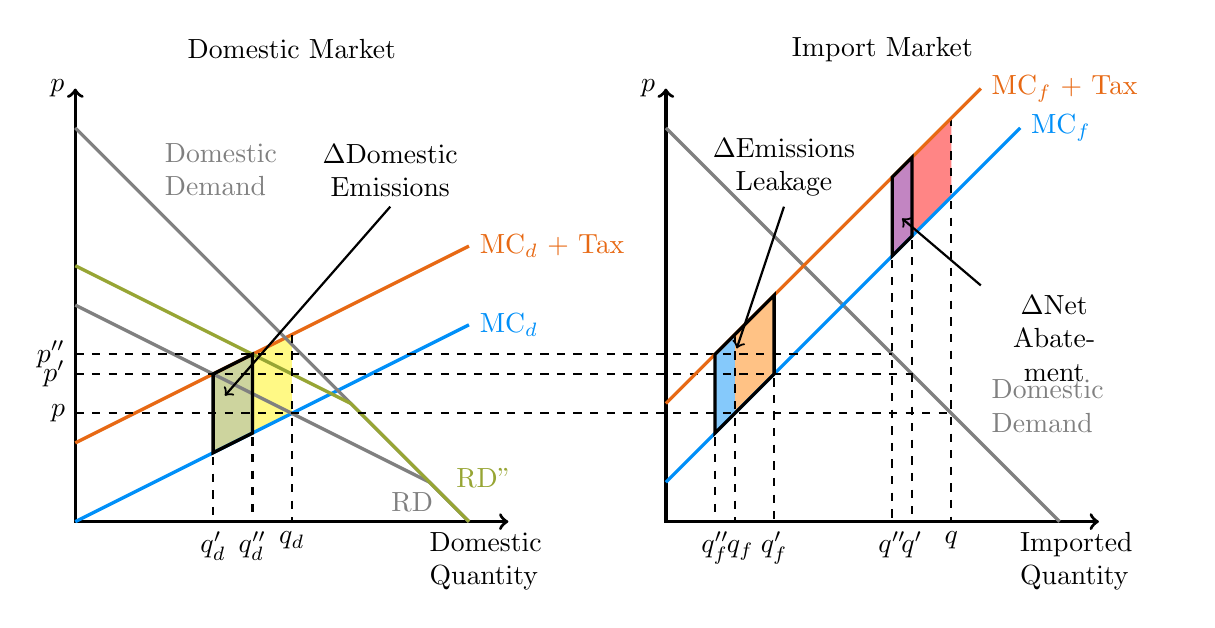
\begin{tikzpicture}[scale = 0.5]
	\draw[very thick, <->] (0, 11) node[left]{$p$} -- (0, 0) -- (11, 0) node[below, text width = 2cm]{Domestic Quantity};
	\draw[very thick, <->] (15, 11) node[left]{$p$} -- (15,0) -- (26, 0) node[below, text width = 2cm]{Imported Quantity};

	\fill[color2!80!, opacity = 0.6] (3.5, 3.75) -- (3.5, 1.75) -- (4.5, 2.25) -- (4.5, 4.25) -- cycle;
	\fill[yellow!80!, opacity = 0.6] (4.5, 2.25) -- (5.5, 2.75) -- (5.5, 4.75) -- (4.5, 4.25) -- cycle;
	\fill[orange!80!, opacity = 0.6] (16.75, 4.75) -- (16.75, 2.75) -- (17.75, 3.75) -- (17.75, 5.75) -- cycle;
	\fill[color1!80!, opacity = 0.6] (16.25, 4.25) -- (16.25, 2.25) -- (16.75, 2.75) -- (16.75, 4.75) -- cycle;
	\fill[red!80!, opacity = 0.6] (21.25, 9.25) -- (21.25, 7.25) -- (22.25, 8.25) -- (22.25, 10.25) -- cycle;
	\fill[violet!80!, opacity = 0.6] (20.75, 8.75) -- (20.75, 6.75) -- (21.25, 7.25) -- (21.25, 9.25) -- cycle;

	\draw[very thick, color1] (0,0) -- (10, 5) node[right]{MC$_d$};
	\draw[very thick, color3] (0,2) -- (10, 7) node[right]{MC$_d$ $+$ Tax};
	\draw[very thick, gray] (0, 10) -- (10,0) node[pos=.2, above right,text width = 1.5cm]{Domestic Demand}; 
	\draw[very thick, gray] (0,5.5) -- (9, 1) -- (10, 0) node[pos=.5, left, xshift = -2pt]{RD};
	\draw[very thick, color2] (0, 6.5) -- (7,3) -- (10, 0) node[pos=.8, above right, text width = 1.5cm]{RD''};
	\draw[very thick, gray] (15, 10) -- (25, 0) node[pos=.8, above right,text width = 1.5cm]{Domestic Demand}; 
	\draw[very thick, color1] (15, 1) -- (24, 10) node[right, text width = 1.5cm]{MC$_f$};
	\draw[dashed, thick] (5.5, 4.75) -- (5.5, 0) node[below]{$q_d$};
	\draw[dashed, thick] (3.5, 3.75) -- (3.5, 0) node[below]{$q_d'$};
	\draw[dashed, thick] (4.5, 4.25) -- (4.5, 0) node[below]{$q_d''$};
	\draw[dashed, thick] (0, 3.75) node[left]{$p'$} -- (21.25, 3.75);
	\draw[dashed, thick] (0, 2.75) node[left]{$p$} -- (22.25, 2.75);
	\draw[dashed, thick] (0,4.25) node[left]{$p''$} -- (20.75, 4.25);
	\draw[dashed, thick] (16.75,4.75) -- (16.75, 0) node[below, yshift = -3pt, xshift = 2pt]{$q_f$};
	\draw[dashed, thick] (17.75, 5.75) -- (17.75, 0) node[below]{$q_f'$};
	\draw[dashed, thick] (16.25, 4.25) -- (16.25, 0) node[below]{$q_f''$};
	\draw[dashed, thick] (22.25, 10.25) -- (22.25, 0) node[below]{$q$};
	\draw[dashed, thick] (21.25, 9.25) -- (21.25, 0) node[below]{$q'$};
	\draw[dashed, thick] (20.75, 8.75) -- (20.75, 0) node[below]{$q''$};
	\draw[color3, very thick] (15, 3) -- (23, 11) node[right]{MC$_f$ $+$ Tax};

	\draw[very thick] (3.5, 3.75) -- (3.5, 1.75) -- (4.5, 2.25) -- (4.5, 4.25) -- cycle;
	\draw[very thick] (16.25, 4.25) -- (16.25, 2.25) -- (17.75, 3.75) -- (17.75, 5.75) -- cycle;
	\draw[very thick] (20.75, 8.75) -- (20.75, 6.75) -- (21.25, 7.25) -- (21.25, 9.25) -- cycle;
	\draw[thick, <-] (3.8, 3.2) -- (8, 8) node[above, text width = 2cm, align=center]{$\Delta$Domestic Emissions};
	\draw[thick, <-] (16.8, 4.4) -- (18, 8) node[above, text width = 2cm, align=center]{$\Delta$Emissions Leakage}; 
	\draw[thick, <-] (21, 7.7) -- (23, 6) node[below right, text width = 1.6cm, align=center]{$\Delta$Net Abatement};
	\node at (5.5, 12) {Domestic Market};
		\node at (20.5, 12) {Import Market}; 
\end{tikzpicture}
\vspace*{1em}
\fignote[1]{
	Residual demand in the domestic market is calculated as the difference between the quantity demanded and the quantity supplied in the import market. Subscripts of $d$ denote a domestic quantity ($q$) or marginal cost (MC), and $f$ denote a foreign quantity or marginal cost. Quantities and prices ($p$) with an $'$ are after the carbon tax has been applied, quantities and prices without an $'$ are before the carbon tax has been applied, and quantities with an $''$ are after the import charge. Different from Figure \ref{leakage_ex}, here importers actually face an identical tax, shifting the marginal costs in the import market to the left. Together, the green and yellow shaded region represent the value of domestic emissions reductions with no import charge, the orange shaded region represents the cost of increases in foreign emissions (i.e., emissions leakage) with no import charge, and the red shaded region represents the value of the net emissions abatement with no import charge. The green shaded region represents the cost ofn increases in domestic emissions, the blue and orange region together represent the value of emissions reductions in foreign emissions, and the violet region represents the value of the increase in net abatement, all associated with the import charge.
}
\end{figure}

% Before we determine how to assess the emissions of imported goods, it is useful to know how we assess the emissions of domestically produced goods. The GHG Protocol, the internationally recognized leader in GHG emissions accounting standards, sets out three emissions scopes. Scope 1 looks at just an organization's direct emissions, like the GHGs that the organization emits on site. Scope 2 includes all these direct emissions from Scope 1, but also includes indirect emissions associated with energy inputs. For instance, a database center might have relatively low Scope 1 emissions, but if all electric power needed for the database center comes from a coal-fueled plant, Scope 2 emissions would be high. Scope 3 takes this a step further to look at the lifecycle emissions associated with an organization. This includes all the emissions captured by Scope 2, and includes emissions embodied in non-energy inputs and downstream emissions from distribution, processing, use, and disposal of its output. Any domestic emissions pricing program first needs to determine what emissions it will use to assess emissions to firms. It is best practice to assess foreign emissions with the same scope as domestic emissions, and likely violates international trade law to assess emissions using a higher scope for foreign producers \citep{cosbey2020developing}.

% \begin{figure}
% 	\caption{Greenhouse Gas Emissions Scopes \citep{ghg_protocol_2011}\label{scopes}}
% 	\centering
% 	\includegraphics[width=0.8\textwidth]{figures/chapter2_figures/ghg_scope.png}
% \end{figure}

In their most complete form, border carbon adjustments cover all goods that cross the border, not just imports. Just like highly-regulated domestic production will likely have a cost disadvantage in the domestic market, highly-regulated exports will likely have a cost disadvantage in foreign markets. To prevent jurisdictions with ambitious climate policy from losing their exports requires some way to adjust the price of exports. This is the purpose of an export rebate, often just called an output rebate.

An output rebate pays back a flat rate to domestic producers for every unit they export. While carbon taxes on imports try to even the playing field between highly regulated and less regulated producers in domestic markets, output rebates try to even the playing field between highly regulated and less regulated producers on foreign markets. For instance, if US fertilizer manufacturers export much of their product, imposing a domestic carbon tax raises these manufacturers' costs relative to their competitors overseas. This cost differential may allow foreign fertilizer manufacturers to retake some of the (foreign) market share from US fertilizer manufacturers. This increased foreign production will lead to greater GHG emissions associated with the foreign fertilizer market, a problem that may be exacerbated if foreign manufacturers were already more emissions intensive than US manufacturers.

Output rebates lack some of the same intuitive appeal that an emissions tax on imports have. After all, why should regulators tax manufacturers only to pay them back? Why not just tax manufacturers the difference between the original emissions tax and the output rebate? The first reason is a matter of accounting. Output rebates only apply to exports, so reducing the tax on all goods would not differentiate between the goods that should and should not receive a subsidy to avoid leakage. The second reason is a matter of incentives. Output rebates are not refunds on emissions taxes, as the government pays these out for every unit of output rather than for every tonne of GHG emissions. In a world where goods had a fixed emissions intensity, this difference would not matter. Thankfully though, there are ways to reduce emissions without reducing output (e.g., switching to cleaner inputs or installing smokestack scrubbers). Thus, an output rebate will maintain the same abatement incentive on exports, while also allowing domestic producers to maintain their ability to compete in foreign markets. The low volume of US manufacturing exports relative to imports means that these are not typically the primary concern in anti-leakage policy.

To summarize, carbon pricing and many other climate policies suffer from their unrequited, unilateral nature. Asymmetric climate regulation provides competitive advantages to firms in less-regulated jurisdictions, a result with a strong backing in theory and evidence for a select number of industries. The two key characteristics of these industries are a high emissions intensity (high ratio of emissions to output) and a high trade exposure (highly traded). In these industries, climate policy can ``leak'' emissions to other jurisdictions, undermining domestic emissions abatement. To combat this, jurisdictions with stringent environmental policy relative to their trading partners can implement border carbon adjustments (BCAs) to reduce regulatory disparities in both domestic and foreign markets. These policies will be key in ensuring that packages of climate policy, including carbon pricing programs, can effectively reduce the global level of emissions.  


% \begin{figure}
% \caption{Leakage with an Emissions Tax on Imports}
% \centering
% \singlespacing
% \footnotesize
% \begin{tikzpicture}[scale = 0.5]
% 	\draw[very thick, <->] (0, 11) node[left]{$p$} -- (0, 0) -- (11, 0) node[below, text width = 2cm]{Domestic Quantity};
% 	\draw[very thick, <->] (15, 11) node[left]{$p$} -- (15,0) -- (26, 0) node[below, text width = 2cm]{Imported Quantity};
% 	\fill[orange!80!, opacity = 0.6] (3.5, 3.75) -- (3.5, 1.75) -- (4.5, 2.25) -- (4.5, 4.25) -- cycle;
% 	\fill[yellow!80!, opacity = 0.6] (4.5, 2.25) -- (5.5, 2.75) -- (5.5, 4.75) -- (4.5, 4.25) -- cycle;
% 	\fill[orange!80!, opacity = 0.6] (16.75, 4.75) -- (16.75, 2.75) -- (17.75, 3.75) -- (17.75, 5.75) -- cycle;
% 	\fill[yellow!80!, opacity = 0.6] (16.25, 4.25) -- (16.25, 2.25) -- (16.75, 2.75) -- (16.75, 4.75) -- cycle;
% 	\fill[orange!80!, opacity = 0.6] (21.25, 9.25) -- (21.25, 7.25) -- (22.25, 8.25) -- (22.25, 10.25) -- cycle;
% 	\fill[yellow!80!, opacity = 0.6] (20.75, 8.75) -- (20.75, 6.75) -- (21.25, 7.25) -- (21.25, 9.25) -- cycle;
% 	\draw[very thick, color1] (0,0) -- (10, 5) node[right]{MC$_d$};
% 	\draw[very thick, color3] (0,2) -- (10, 7) node[right]{MC$_d$ $+$ Tax};
% 	\draw[very thick, gray] (0, 10) -- (10,0) node[pos=.2, above right,text width = 1.5cm]{Domestic Demand}; 
% 	\draw[very thick, color2] (0,5.5) -- (9, 1) -- (10, 0) node[pos=.8, above right, text width = 1.5cm]{Residual Demand};
% 	\draw[very thick, color2] (0, 6.5) -- (7,3) -- (10, 0);
% 	\draw[very thick, gray] (15, 10) -- (25, 0) node[pos=.8, above right,text width = 1.5cm]{Domestic Demand}; 
% 	\draw[very thick, color1] (15, 1) -- (24, 10) node[right, text width = 1.5cm]{MC$_f$};
% 	\draw[dashed, thick] (5.5, 4.75) -- (5.5, 0) node[below]{$q_d$};
% 	\draw[dashed, thick] (3.5, 3.75) -- (3.5, 0) node[below]{$q_d'$};
% 	\draw[dashed, thick] (4.5, 4.25) -- (4.5, 0) node[below]{$q_d''$};
% 	\draw[dashed, thick] (0, 3.75) node[left]{$p'$} -- (21.25, 3.75);
% 	\draw[dashed, thick] (0, 2.75) node[left]{$p$} -- (22.25, 2.75);
% 	\draw[dashed, thick] (0,4.25) node[left]{$p''$} -- (20.75, 4.25);
% 	\draw[dashed, thick] (16.75,4.75) -- (16.75, 0) node[below, yshift = -3pt, xshift = 2pt]{$q_f$};
% 	\draw[dashed, thick] (17.75, 5.75) -- (17.75, 0) node[below]{$q_f'$};
% 	\draw[dashed, thick] (16.25, 4.25) -- (16.25, 0) node[below]{$q_f''$};
% 	\draw[dashed, thick] (22.25, 10.25) -- (22.25, 0) node[below]{$q$};
% 	\draw[dashed, thick] (21.25, 9.25) -- (21.25, 0) node[below]{$q'$};
% 	\draw[dashed, thick] (20.75, 8.75) -- (20.75, 0) node[below]{$q''$};
% 	\draw[color2, very thick] (15, 3) -- (23, 11) node[right]{MC$_f$ $+$ Tax};
% 	%\draw[thick, <-] (5, 4) -- (8, 8) node[above, text width = 2cm, align=center]{Domestic Abatement};
% 	%\draw[thick, <-] (16.7, 4.5) -- (18, 8) node[above, text width = 2cm, align=center]{Emissions Leakage}; 
% 	%\draw[thick, <-] (21.6, 8) -- (23, 6) node[below right, text width = 1.6cm, align=center]{Net Abatement};
% 	\node at (5.5, 12) {Domestic Market};
% 	\node at (20.5, 12) {Foreign Imports}; 
% \end{tikzpicture}
% \end{figure}

% %%%%%%%%%%%
\newpage
\section{Ambient Air Pollution \& Electricity Generation}

The previous two chapters have focused on preparing a broad base of knowledge on climate economics---the first chapter by reviewing the physical science of climate change and the second chapter by reviewing the economics of climate policy design. This chapter continues to build background, but focuses instead on providing context specific to the modeling and empirical work done in the two chapters that follow it. 

To motivate these proceeding chapters, this chapter begins by discussing ambient air pollution with particular emphasis on the impacts of ambient air pollution and air pollution disparities. As alluded to earlier, the ultimate goal is to model and simulate these air pollution disparities that result from the implementation of a carbon tax on the electric power industry in California. Keeping this in mind, the discussion on air pollution is followed by an overview of wholesale electricity markets and Assembly Bill 32 (AB-32), the California statute that creates an emissions trading program across the state. Finally, I review the body of literature immediately adjacent to this research. The related literature serves both to establish what we already know about the implications of carbon pricing for environmental inequality and to motivate the specific goals of the research in this paper. This chapter concludes by describing the overall research design that unfolds in the next two chapters. The description of this design is outlines both the research design choices I make in these later chapters and the motivation for these design choices. 

\subsection{Primer on Ambient Air Pollution}

\noindent Introduction
\begin{itemize}
    \item What is ambient air pollution? 
    \item What are the most common air pollutants?
\end{itemize}

Ambient air pollution exposure comes with many negative consequences, but the most striking of these is the effect of ambient air pollution on human health and mortality. \textbf{Talk about the mechanisms using \cite{aguilar2022air}}.

The World Health Organization (WHO) estimates that ambient air pollution caused over 4.2 million premature deaths in 2019, making ambient air pollution one of the leading global health stressors \citep{who_factsheet}. Around the world, 99\% of people live in environments that do not meet the WHO's air quality guidelines. Understandably, the vast majority (89\%) of these premature deaths are in low- and middle-income countries, but ambient air pollution remains a serious health threat even in wealthy nations, including the US. \cite{lelieveld2019effects} uses atmospheric models alongside a global exposure mortality model---a model that maps air pollutant concentrations into mortalities---to study excess mortalities attributable to anthropogenic air pollution emissions. They find that ambient air pollutants from anthropogenic sources (primarily the burning od fossil fuels) result in 230,000 excess deaths annually in the US.\footnote{
    The 95\% confidence interval around these estimates is 184,000--276,000 excess deaths---a wide interval, but an interval where even the minimum of the interval warrants serious concern.
} 

Apart from the devastating effects of air pollution on human health, the other primary effect of air pollution exposure is reduced cognitive performance and decision making. \cite{fonken2011air} find physical changes in the brains of mice who have been exposed to fine particulate matter at concentrations and durations comparable to Beijing. Namely, they find that neurons in the hippocampus---an area of the brain devoted to memory and learning---have shorter and less dense dendrites. These dendrites are responsible for receiving signals from other neurons, and the reduced length and density of these neurons is correlated with poorer memory \citep{weir2012smog}.Additionally, the mice exposed to particulate matter display depressive-like symptoms, giving up earlier in forced swimming tests and eating less. 

These physiological findings in mice correspond with a wealth of evidence on the effects of air pollution on human learning and cognition. \cite{aguilar2022air} provides the best review of these effects and their implications for human capital formation and labor economics more broadly. 

\noindent Education/Human Capital Development \& Labor Implications
\begin{itemize}
    \item \cite{zhang2018impact}
    \item \cite{currie2014we}
    \item \cite{aguilar2022air}
    \item \cite{currie2009does}
    \item \cite{ebenstein2016long}
    \item \cite{chang2016particulate}
\end{itemize}




\noindent Crime
\begin{itemize}
    \item \cite{bondy2020crime}
    \item \cite{burkhardt2019effect}
\end{itemize}

\noindent Happiness
\begin{itemize}
    \item \cite{zheng2019air}
\end{itemize}

Together, the many effects of air pollution add to the popular 






\noindent Justice/Inequality/Distributional perspectives
\begin{itemize}
    \item \cite{colmer2020disparities}
    \item \cite{hernandez2022decomposing}
    \item \cite{currie2023caused}
    \item \cite{banzhaf2019environmental}
    \item \cite{voorheis2017air}
\end{itemize}






\subsection{The Case of California: Electricity \& AB-32}

\begin{figure}
    \centering
    \caption{Western Interconnection Subregions}
    \includegraphics[width=0.8\textwidth]{figures/chapter3_figures/WECC_map.pdf}
    \fignote[1]{Figure displays the subregions of the Western Interconnection. These subregions are a unit of geography set by the North American Electric Reliability Council (NERC). NERC determines these regions based off of the connections/boundaries between balancing authorities, the administrative unit of the US power grid. These regions are the California-Mexico Power Area (CAMX), the Northwest Power Pool Area (NWPP), the Rocky Mountain Power Area (RMPA), and the Arizona-New Mexico-Southern Nevada Power Area (AZNM). The EPA reports data for each of the four NERC regions, but the EIA only provides electricity demand data for the NWPP and RMPA together. These two subregions are treated as one throughout the paper, and future chapters will model just the three regional markets displayed: the California market, the Southwest market, and the Northwest market. Shapefiles for the regions come from \cite{HIFLD_nerc}.
    }
\end{figure}

\begin{figure}
    \centering
    \caption{California Emissions Allowance Price}
    \includegraphics[width=\textwidth]{figures/chapter3_figures/allowance_prices.pdf}
    \fignote[1]{Figure displays the auction price and price floor for emissions allowances in California from Q4 2015 through Q4 2022. Each emissions allowance covers one tonne of CO$_2$e emissions. Data on emissions allowances come from the California Air Resources Board, \cite{carb_prices}.}
\end{figure}


\noindent Wholesale electricity markets: How they work and their ``competitiveness"
\begin{itemize}
    \item \cite{ferc2020}
\end{itemize}

\noindent Short history of CAISO
\begin{itemize}
    \item \cite{sweeney2013california}
    \item \cite{knittel2005empirical}
    \item \cite{borenstein2000diagnosing}
    \item \cite{borenstein2015us}
\end{itemize}

\noindent Leakage
\begin{itemize}
    \item \cite{burtraw2018}
    \item \cite{fowlie2009incomplete}
    \item \cite{fowlie2021border}
\end{itemize}

\noindent Effect of AB-32 on Electricity
\begin{itemize}
    \item \url{https://ww2.arb.ca.gov/our-work/programs/cap-and-trade-program/cap-and-trade-
    regulation}
\end{itemize}

\subsection{Carbon Pricing \& Environmental Inequality}

Carbon pricing policies are highly popular among economists. In what is likely the greatest display of consensus on climate policy from the economics discipline, most all of the nation's leading economists endorsed a series of policy recommendations published in the Wall Street Journal in 2019. The statement titled ``Economists' Statement on Carbon Dividends" calls for the implementation of a nationwide tax on greenhouse gas emissions, border carbon adjustments, and carbon dividends to redistribute the collected tax revenue. Original signatories of the statement include twenty-eight Nobel Laureates, four former Chairs of the Federal Reserve, and fifteen former Chairs of the Council of Economic Advisors. Since its initial release, the statement has earned the signature of thousands of other economists.\footnote{This includes many other well-known economists, like Susan Athey, Daron Acemoglu, and Rick Eichhorn.}

As discussed in Chapter 2, the primary appeal of carbon pricing for economists is the cost-minimizing nature of these policies. The consensus statement's first policy recommendation states this unambiguously:
\begin{quote}
    ``A carbon tax offers the most cost-effective lever to reduce carbon emissions at the scale and speed that is necessary. By correcting a well-known market failure, a carbon tax will send a powerful price signal that harnesses the invisible hand of the marketplace to steer economic actors towards a low-carbon future." 
\end{quote}




It is also relevant to note that the signing economists address how the revenue generated from the carbon price should be distributed---an aspect that if done poorly could create major inequality concerns. The statement's fifth and final policy recommendation reads: 
\begin{quote}
    ``To maximize the fairness and political viability of a rising carbon tax, all the revenue should be returned directly to U.S. citizens through equal lump-sum rebates. The majority of American families, including the most vulnerable, will benefit financially by receiving more in `carbon dividends' than they pay in increased energy prices."
\end{quote}
Together the policy recommendations in the statement provide a brief but clear strategy for reducing greenhouse gas emissions in a manner that is both efficient and progressive in the sense that tax revenue would flow towards those at the bottom end of the income distribution. 

Despite the carbon-pricing fervor of economists, many in the climate policy community remain skepitcal of proposals that rely heavily on carbon pricing for decarbonization. There are a number of arguments against carbon pricing that critique the efficacy of these programs relative to their alternatives, but these concerns are not new and generally struggle to make a strong case.\footnote{Chapter 2 describes arguments against carbon pricing that critique the efficacy of these programs. This discussion comes to four primary conclusions. First, there is a need for additional research that measures the ex-post effect of carbon pricing on emissions reductions. Second, many jurisdictions with carbon pricing programs have chosen to rely on other regulations to attain emissions targets. That is, the implicit price on emissions from other regulations is often higher than the market price of emissions, which can make the effect of emissions pricing appear weak relative to other regulations. Third, in situations where policymakers rely primarily on carbon pricing more so than other regulations, carbon pricing does appear to be the more cost-effective policy. This difference appears to be small though, especially in the electricity market where the strong correlation between the merit order of generation and emissions intensity mean that clean energy standards perform only negligibly worse carbon pricing. Fourth, there are likely tangible improvements to emissions trading programs that can be made, such as reforming or eliminating the use of emissions offsets. 
} Instead, more recent criticism of these policies has centered around their potential to perpetuate environmental inequality. Because global air pollutants (i.e., greenhouse gases) are often released at the same time as local air pollutants (i.e., criteria air pollutants, including PM, NO$_x$, SO$_2$), carbon pricing has the potential to shift the distribution of ambient air pollution. In this context, the less-regulated local air pollutants are often called copollutants. The concern is that even if environmental markets can induce abatement efficiently, the ``invisible hand'' economists celebrate might just shift the burden of air pollution towards already disadvantaged communities. Raising this possibility is entirely fair. After all, the decentralized nature of market means there is no specific mechanism to prevent this from happening. The most vulnerable in society may already feel disenfranchised by market-systems, so the resistance to a cap-and-trade program---a market-based policy instrument---is not entirely surprising. 

Many Californians have expressed concerns about the potential for California's cap-and-trade program to redistribute the air pollution burden towards communities with already poor environmental quality and economic status. In fact, the first question on the ``Frequently Asked Questions'' page of California's cap-and-trade program's website reads: ``Does the cap-and-trade program lead to increases of air pollution in environmental justice communities burdened with air pollution?'' \citep{carb_FAQ}. This was not a major concern when AB-32 was originally passed in 2006, but nearly ended California's cap-and-trade program when it needed to be reauthorized ten years later in 2016 \citep{johnson2020cap}. 

% \citep{johnson2020cap} recounts the political drama surrounding the 2016 reauthorization of California's cap-and-trade program, where many environmental justice advocates pushed for more localized controls air pollutants

% It is important to be clear about the tradeoff this analysis looks at. 

% There is a separate political tradeoff 
% \begin{quote}
%     Most environmental justice advocates aren't fundamentally opposed to putting a price on carbon; they are opposed to the political pattern, repeated several times over, where politicians trade away working local air pollution laws to tackle the global problem of climate change.
% \end{quote}

% The goal of this analysis is not to , 

% Economists \emph{love} carbon pricing, others are less keen (distributional reasons)
% \begin{itemize}
%     \item \cite{fischer2021green}
%     \item \cite{borenstein2022carbon}
% \end{itemize}

% \begin{itemize}
%     \item \url{https://grist.org/climate/the-biggest-fight-over-cap-and-trade-isnt-about-what-you-think-it-is/}
%     \item \url{https://ww2.arb.ca.gov/resources/documents/faq-cap-and-trade-program}
% \end{itemize}

These concerns were intensified following the release of several descriptive analyses that seemed to indicate that California's cap-and-trade program had done exactly that: redistributed air pollution towards disadvantaged communities. \cite{cushing2018carbon}, circulated at the time as \cite{cushing2016preliminary}, notes that even though total emissions from regulated facilities decreased in the three years after the implementation of California's cap-and-trade program, 52\% of facilities actually increased their emissions. Further, \cite{cushing2018carbon} finds that the communities with increases in co-pollutant emissions are on average poorer, less educated, and have a higher proportion of non-white residents than communities with decreases in co-pollutant emissions. In a follow-up study with a few additional years worth of data, \cite{pastor2022up} found similar results. The median facility covered by the cap-and-trade program in a disadvantaged community increased its PM10 emissions by 3.1\%, while the median facility covered by the cap-and-trade program in a non-disadvantaged community decreased its PM10 emissions by 6.9\%---a 10 percentage point difference in changes of PM10 emissions. Other air pollutants show similar disparities in pollution changes, though these differences are only statistically significant at the 5\% level for PM10 and SO$_x$, not for PM2.5, NO$_x$, or greenhouse gas emissions themselves. 

While these two studies help establish important descriptions of environmental justice outcomes in California, as \cite{hernandez2022importance} note, these do little to speak to the actual effect of the cap-and-trade program. First, their results cannot disentangle the effects of the cap-and-trade program from contemporaneous events that may cause the redistribution of co-pollutants. Pollution intensive activities are highly responsive to macroeconomic trends, and it is entirely possible that the redistribution of co-pollutants towards disadvantaged communities is a consequence of these macroeconomic trends rather than the effects of the cap-and-trade program. Second, co-pollutants are often not stagnant, but move into neighboring communities based on geography and atmospheric conditions. This means that even if the emissions of co-pollutants increases in a community, this is not sufficient information to suggest that the air pollution exposure in that community increases as well. 

\cite{hernandez2023environmental} is the first study to provide credible causal measurements of the impact of the cap-and-trade program on air pollution exposure. The authors define and measure changes in the ``environmental justice gap,'' the average difference in air pollution concentrations between disadvantaged and other communities.\footnote{California designates certain census tracts as ``disadvantaged” as a part of the CalEnviroScreen.} In contrast to \cite{cushing2018carbon} and \cite{pastor2022up}, Hernández-Cortés and Meng find evidence that California's cap-and-trade program actually reduced the environmental justice gap, by 6-10\% annually. Hernández-Cortés and Meng address the two limitations of earlier descriptive analysis by (1) using a difference-in-differences model that makes use of the staggered implementation of the cap-and-trade program to disentangle the effects of the cap-and-trade program from other contemporaneous events, and (2) embedding the predicted facility-level co-pollutant emissions within a chemical transport model that allows them to accurately measure air pollution exposure. Although Hernández-Cortés and Meng find evidence the cap-and-trade program has reduced disparities in air pollution exposure, they are also careful to emphasize that a cap-and-trade is not necessarily the sufficient to reduce these disparities. Nonetheless, their results suggest that Californians need not worry that the State's cap-and-trade program will exacerbate existing disparities in air pollution exposure. 

% \noindent Causal analysis
% \begin{itemize}
%     \item \cite{hernandez2023environmental}
%     \item \cite{hernandez2021environmental}
% \end{itemize}

The previously mentioned literature studying the effects of carbon pricing on air pollution disparities has all focused on ex-post analysis of such policies. While retrospective research is vital to ensuring the success of California's cap-and-trade program going forward, the highly contextualized nature of the analysis makes the external validity of these results questionable. The econometric analysis cannot describe any underlying mechanisms that produce the measured causal effects, and without a clear understanding of \emph{how} California's cap-and-trade program helped to close disparities in air pollution exposure, we cannot anticipate the effects of similar policies applied elsewhere. 

\cite{weber2021dynamic} offers, to my knowledge, the first and only ex-ante model that studies how carbon pricing in California affects the spatial redistribution of co-pollutants. The model focuses on the State's electric power industry and follows in the spirit of related structural, industrial-organization models \citep[e.g.,~][]{gowrisankaran2022policy, abito2022role}. Although Weber focuses primarily on the total welfare effects of the redistribution of co-pollutants, her results suggest that counties with more ``disadvantaged” communities appear to also see greater reductions in co-pollutant emissions. These findings pair well with those in \cite{hernandez2023environmental}, although Weber focuses on only power plants and Hernández-Cortés and Meng focus on all regulated facilities except power plants.

% \noindent The IO approach
% \begin{itemize}
%     \item \cite{weber2021dynamic}
%     \item \cite{gowrisankaran2022policy}
%     \item \cite{abito2022role}
%     \item \cite{cullen2017}
%     \item \cite{cullen2015}
% \end{itemize}

% \noindent Distributional considerations with incomplete regulation
% \begin{itemize}
%     \item \cite{hernandez2022distributional}
%     \item \cite{tanaka2022north}
% \end{itemize}


\subsection{Research Design}




% \subsection{A Perfectly Competitive Model of Leakage}

% Here we consider a perfectly competitive model of emissions leakage in the Western Interconnection based largely off of \cite{fowlie2021border}. We begin constructing a model where there is no emissions pricing scheme and then impose an emissions tax. Alongside the emissions tax, we consider different possible border carbon adjustments with the potential to reduce leakage. 

% This is not a model of residential electric power markets. Residential electric power prices involve complicated tier systems, connection charges, and many additional fees that distort the true price. In addition to discouraging electrification \citep[see][]{borenstein2021designing}, these structures make simulating these markets impractical in this analysis. Instead, we model the wholesale day-ahead electricity market. 

% The Federal Energy Regulatory Commission's \emph{Energy Primer} \citep{ferc2020} describes how power grid operators and power plants decide what generation will take place. Power grid operators have the goal of ensuring reliable power supply at the least cost. This process plays out in two stages. In the first stage, operators prepare for forecasted demand by committing generators a day before. This is the day-ahead market, where power plants sell their generation in anticipation for the next day. In the second stage, operators make adjustments in real-time by calling on additional generators to either turn on or off through a process called Automatic Generation Control. Grid operators determine whether or not to increase generation by measuring the frequency (cycles/second) of the AC power lines. In the US, operators aim for a frequency of 60 Hz, so a frequency above or below 60 Hz means that the too much or too little generation respectively. 

% The structure of these day-ahead markets varies considerably across the country. One important factor in identifying the structure of these markets is the existence of a Regional Transmission Operator (RTO) or an Independent System Operator (ISO). RTOs and ISOs are essentially two different names for the same entity.\footnote{\cite{rff_podcast1} says ``At one point, FERC---the Federal Energy Regulatory Commission---made a distinction between these entities. It's a distinction without a difference at this point."} These entities are non-profit organizations that have the primary responsibility of operating markets for electric power
% across many generators (the power plants, i.e. the sellers of electricity) and load-serving organizations (utilities, large industrial users, i.e. the buyers of electricity). \cite{ferc2020} gives an excellent description of how these day-ahead markets operate under an RTO or ISO.
% \begin{quote}
% In day-ahead markets, the schedules for supply and usage of energy are compiled hours ahead of the beginning of the operating day. The RTO/ISO then runs a computerized market model that matches buyers and sellers throughout the market footprint for each hour throughout the day. The model then evaluates the bids and offers of the participants, based on the power flows needed to move the electricity throughout the grid from generators to consumers. Additionally, the model must account for changing system capabilities that occur, based on weather and equipment outages, plus the rules and procedures that are used to ensure system reliability. The market rules dictate that generators submit supply offers and that loads submit demand bids to the RTO/ISO by a deadline that is typically in the morning of the day-ahead scheduling. Typically, 95 percent of all load is scheduled in the day-ahead market and the rest is scheduled in real-time.
% \end{quote}
% This means that the wholesale day-ahead market has many of the characteristic features of a competitive market. The good bought and sold is homogeneous, and buyers have little ability to differentiate between  sellers. There are thousands of power plants selling power in any RTO/ISO and dozens of utilities and industrial costumers buying it. Moreover RTOs/ISOs dispatch additional generating units based on their marginal costs, which is suggestive that supply in the market is allocated competitively. Given this market structure, it seems most sensible to model this market as perfectly competitive. 

% \subsubsection*{The General Model}

% Consider a model of the Western Interconnection. Denote the set of all power plants in the interconnection as $N$ and the subset of power plants located in California with $N_\text{Cal}$. The set of regions $R$ in the interconnection, each with its own market for electric power and its own generation. For now, assume these markets behave competitively. Further, assume that plants in each regional market face linear inverse demand curves with the form
% \begin{equation}
% 	p_r = \alpha_r - \beta_r Q_r
% \end{equation}
% where $p_r$ is the price in region $r$ (\$/MWh), $Q_r$ is the total quantity of power demanded in region $r$ (MWh), and $\alpha_r$ and $\beta_r$ are regional constants. 

% Each power plant decides how much power to generate for each regional market. Let $q_{ir}$ denote the power in MWh that plant $i$ generates to sell in regional market $r$. Any plant can generate power for any other region, regardless of what region the plant is located in. 

% We can group all power plants into one of two groups: fossil fuel plants and non-fossil fuel plants. Fossil fuel plants each have a plant specific marginal cost that depends on some of the physical features of its generators and the cost of the fuel it uses (natural gas, coal, or occasionally, oil). Fossil fuel plants choose how much power to generate based on their marginal costs and the prices in each market. 

% Non-fossil fuel plants do not have such clear marginal costs. For instance, a windfarm does not decide how much power to generate based on its marginal cost, but is constrained the generate whatever the environment allows it to. We make the assumption that the total generation for any individual non-fossil fuel plant is fixed, and they have not marginal cost. Note that although the total generation of these plants is fixed, the allocation of their generation is not. These plants can still choose how much of their power to sell in each region. 

% While we might usually endow individual firms with behaviors (objective functions) and try to solve analytically for their aggregate outcome, here we endow the entire interconnection with a behavior instead. Standard economic theory says that the perfectly competitive outcome uniquely maximizes total surplus. Then to simulate this market, we need to find what generation and allocation from each plant maximizes the sum of the areas under the demand curve in each regional market minus any marginal costs, including costs from congestion, carbon taxes, and BCAs. The area under the demand curve in region $r$ is a trapezoid with area
% $$\frac12 \left[\alpha + \left( \alpha_r - \beta_r Q_r^*\right)\right] Q_r^* = \frac12 \left( 2\alpha_r - \beta_r \sum_{i \in N} q_{ir} \right) \sum_{i \in N} q_{ir}$$
% where $Q_r^*$ is the equilibrium quantity regional market $r$. This leads the the optimization problem:
% \begin{align*}
% \max_{\{q_{ir}\}} \hspace{2em}\left\{\sum_{r\in R} \left[ \frac12 \left( 2\alpha_r - \beta_r \sum_{i \in N} q_{ir} \right) \sum_{i \in N} q_{ir}\right] - \left(\sum_{(i, r) \in N \times R} c_i q_{ir}\right) - \tau \left(\sum_{(i, r) \in N \times R} \widetilde{e_{ir}} q_{ir}\right)\right\}
% \end{align*}
% where $\tau$ is the emissions tax (\$/ton of CO$_2$e) and $\widetilde{e_{ir}}$ is the assessed emissions intensity. This assessed emissions intensity is the emissions intensity that policies tax at. As we lay out next, each policy functions by changing what the assessed emissions intensity is for each plant-region pair. The first term in the objective function is the sum of the areas under the demand curves. The second term is the total total marginal operating cost, and the third term is the total emissions cost. The optimization problem is subject to the following constraints:
% \begin{gather*}
% 	q_{ir} \geq 0, ~\text{for all plants} ~i~ \text{and regions} ~r\\
% 	\sum_{r \in R} q_{ir} \leq q_i^\text{max}, ~\text{for all fossil fuel plants} ~i\\
% 	\sum_{r \in R} q_{ir} = \overline{q}_i, ~\text{for all non-fossil fuel plants} ~i\\
% 	\left(\sum_{i \in N_{r}} q_{is}\right)  + \left(\sum_{i \in N_s} q_{ir}\right) \leq T_{(r,s)}, ~\text{for all}~(r,s) \in N\times N ~\text{such that}~ r \neq s
% \end{gather*}
% The first constraint guarantees that plants do not try to generate negative power for a region---they can only generate power at their own plant. The second constraint restricts fossil fuel power plants to their maximum generation (i.e., their nameplate capacity). Non-fossil fuel power plants do not have marginal costs, so the third constraint set the total generation of a non-fossil fuel plant to an exogenous quantity. The final constraint is the transmission constraint. This says that for any two distinct regions $r$ and $s$, the sum of their exports to the other region cannot exceed the maximum transmission load of the lines between them $T_{(r,s)}$. If there were no transmission constraints, nearly total leakage would be  practically guaranteed as trade is completely exposed.

% \begin{table}
% \caption{Notation Summary}
% \centering
% \begin{tabular}{c p{10cm}}
% \hline\hline
% Notation & Description \\
% \hline
% 	$N$ & Set of power plants\\
% 	$R$ & Set of regions\\
% 	$i$ & Subscript denoting an arbitrary power plant, $\i \in N$\\
% 	$r$ & Subscript denoting an arbitrary region, $r \in R$\\
% 	$q_{ir}$ & Plant $i$'s generation to sell in region $r$ (MWh)\\
% 	$q_i^\text{max}$ & Fossil fuel plant $i$'s exogenously determined maximum generation (MWh)\\
% 	$\overline{q}_i$ & Non-fossil fuel plant $i$'s exogenously determined total generation (MWh)\\
% 	$p_r$ & Market price in region $r$\\
% 	$Q_r$ & Generation to sell in region $r$, $Q_r = \sum_{i=1}^N q_{ir}$\\
% 	$e_i$ & Actual emissions intensity of plant $i$ (tons CO$_2$e)\\
% 	$\widetilde{e_{ir}}$ & Assessed emission intensity; emissions intensity for tax purposes of plant $i$ selling in region $r$\\
% 	$d$ & Default emissions intensity\\
% \hline	\hline
% \end{tabular}
% \end{table}

% \subsubsection*{Scenario A: No Regulation}

% Under no regulation, policymakers do not assess emissions to any power plant. That is, $\widetilde{e_{ir}} = 0$.

% \subsubsection*{Scenario B: Complete Regulation}

% Under complete regulation, all plants pay a tax based on their actual emissions intensity in each market. Then set $\widetilde{e_{ir}} = e_i$ for each $i \in N$ and $r \in R$. 

% \subsubsection*{Scenario C: California Carbon Tax, No BCA}

% In this scenario, California implements a domestic carbon tax without a BCA. This means that all plants in California pay a tax based on their actual emissions intensity, but no other plants pay an emissions tax. Then set
% \[
% \widetilde{e_{ir}} = \begin{cases}
% 	~~e_i & \text{if}~~i\in N_\text{Cal}\\
% 	~~0 & \text{if}~~i\not\in N_\text{Cal}.
% \end{cases}
% \]

% \subsubsection*{Scenario D: California Carbon Tax, Uniform BCA}

% Once again, all plants in California face a domestic carbon tax and pay based on their actual emissions intensity. With the uniform BCA though, all plants outside of California pay an emissions tax on the power they export to California. Regardless of their actual emissions intensity, all plants exporting power to California face a default emissions intensity, $d$. In this scenario,
% \[
% \widetilde{e_{ir}} = \begin{cases}
% 	~~e_i & \text{if}~~i\in N_\text{Cal}\\
% 	~~d & \text{if}~~i\not\in N_\text{Cal} ~~\text{and}~~ r = \text{California}\\
% 	~~0 & \text{if}~~i\not\in N_\text{Cal} ~~\text{and}~~ r \neq \text{California}.
% \end{cases}
% \]

% \subsubsection*{Scenario E: California Carbon Tax, Differentiated BCA}

% Lastly, this scenario models a differentiated BCA. The assessed emissions intensities of all California plants is again their actual emissions intensity. Plants outside of California can choose to either pay their actual emissions intensity the default emissions rate, $d$. Assume that plants always choose the lower emissions intensity, so that clean plant with $e_i < d$ will choose to pay using their actual emissions rate and dirty plants with $e_i \geq d$ will choose to pay using the default emissions intensity. This means,
% \[
% \widetilde{e_{ir}} = \begin{cases}
% 	~~e_i & \text{if}~~i\in N_\text{Cal}\\
% 	~~e_i & \text{if}~~i\not\in N_\text{Cal} ~~\text{and}~~ r = \text{California} ~~\text{and}~~ e_i < d \\
% 	~~d & \text{if}~~i\not\in N_\text{Cal} ~~\text{and}~~ r = \text{California} ~~\text{and}~~ e_i \geq d \\
% 	~~0 & \text{if}~~i\not\in N_\text{Cal} ~~\text{and}~~ r \neq \text{California}.
% \end{cases}
% \]


% \subsection{Data}

% Estimating the simulation requires data on all individual power plants, regional electric power markets, and transmission across the entire Western Interconnection. 

% Regional market data comes from US Energy Information Administration's (EIA) Hourly Electric Grid Monitor from 2019. I pull daily generation data by region and by fuel type for the Western Electric Coordinating Council, which governs the Western Interconnection. This aggregates the Western Interconnection into three regions: California, the Northwest, and the Southwest. Additionally, I pull price data from spot markets in each of these regions from the Inter-Continental Exchange (ICE) for the  247 days it is available in 2019. 

% Power plant data comes from the EPA's 2019 Emissions \& Generation Resource Integrated Database (\href{https://www.epa.gov/egrid/download-data}{eGRID}). This database contains annual summary statistics for each power plant in the US, including valuable information on annual emissions, generation, nameplate capacity (maximum generation), location, and fuel type. 


% \subsection{Simulation}

% To simulate the model, we use the CVXR package in R to solve the optimization problem for each day with data in 2019 under each of the different scenarios. 

% Before we can solve these optimization problems, we first need to calibrate several important parameters and exogenous variables. Following the approach of \cite{fowlie2021border}, I choose to set an elasticity of 0.075 for the demand curve at the observed price and quantity in the regional market, and then solve for the values of $\alpha_r$ and $\beta_r$ so that the demand curve each day will pass through the observed price and quantity. Future work will take a more rigorous approach to estimating these daily demand curves. We do not have the data to say what the individual generation of each non-fossil fuel plant was on each day. We do have regional data on the generation by fuel type though, so to make up for this, I fixed the daily generation of non-fossil fuel plants to be proportional to the total generation by the corresponding fuel type. The proportion for each plant is ratio of the nameplate capacity of the individual plant to the total nameplate capacity of all plants with the same fuel type in the region. For instance, suppose on a given day there was a total of 100 MWh generated from wind power in California. Then for a wind farm in California with 10\% of the total nameplate capacity for all wind farms in California, we set $\overline{q} = 10$. 

% I try to use values for the tax rate $\tau$ and the default emissions rate that are historically accurate. I set $\tau = \$19$ per ton, and set $d = 0.428$ tons per MWh. The next five tables compare the simulated annual generation from fossil fuel plants to the actual (observed) generation from these plants  over the same time period. For now, I use the simple regression:
% $$\text{Observed Generation} = \alpha + \beta \cdot \text{Simulated Generation}.$$
% If the simulation model matches the world reasonably well, then the simulated generation amounts should be similar to the observed generation amounts such that $\hat{\alpha} = 0$ and $\hat{\beta} = 1$. If $\hat{beta} > 1$, this indicates that simulated generation tends to be less than actual generation, and if $\hat{beta} < 1$, this indicates that simulated generation tends to be more than actual generation. We expect that the simulated policy that matches most closely to the actual policy (uniform BCAs, simulation D) is closest. 

% Tables 12 and 13 display the primary results of interest. In Table 12, we see the reduction in generation in each region by fuel type for each of the different policy simulations from the baseline scenario where there is no carbon pricing scheme. These results indicate substantial leakage when there is a carbon tax in California, but no BCA (Simulation C). California reduces its generation from natural gas substantially, as most of its power comes from natural gas. This results in large increases in both natual gas and coal generation in the Southwest. In Simulation E (Differentied BCA), we see that there is still substantial leakage as it appears low emissions intensity generation in the southwest is redirected to California. Uniform BCAs though appear much more successful in reducing emissions. These early results are consistent with our intuition of the apparent risks for reshuffling under differentiated BCAs. 

% \singlespacing
% \newpage
% \begin{table}[!htbp] \centering 
%   \caption{Annual Generation from Simulation A} 
% \begin{tabular}{@{\extracolsep{5pt}}lccc} 
% \hline \hline \\[-1.8ex]
%  & \multicolumn{3}{c}{Actual Generation (MWh)} \\ 
% \\[-1.8ex] & All Fossil Fuel & Natural Gas & Coal\\ 
% \hline \\[-1.8ex] 
%  Simulated Generation (MWh) & 1.035$^{***}$ & 0.769$^{***}$ & 1.192$^{***}$ \\ 
%   & (0.039) & (0.038) & (0.150) \\ 
%   & & & \\ 
%  Constant & 233,326.600$^{***}$ & 227,964.100$^{***}$ & 1,216,915.000$^{**}$ \\ 
%   & (51,713.200) & (40,188.380) & (459,448.200) \\ 
%   & & & \\ 
% Observations & 505 & 448 & 40 \\ 
% R$^{2}$ & 0.578 & 0.476 & 0.623 \\ 
% \hline \\[-1.8ex] 
% \textit{Notes:} & \multicolumn{3}{l}{$^{***}$Sig. at 1\% level, $^{**}$Sig. at 5\% level}, $^{*}$Sig. at 10\% level \\
% \end{tabular} 
% \end{table} 

% \begin{figure}
% 	\centering
% 	\caption{Annual Generation in Simulation A}
% 	\includegraphics[width=0.8\textwidth]{figures_4/p1A.png}
% \end{figure}



% \begin{table}[!htbp] \centering 
%   \caption{Annual Generation from Simulation B} 
% \begin{tabular}{@{\extracolsep{5pt}}lccc} 
% \hline \hline \\[-1.8ex] 
% & \multicolumn{3}{c}{Actual Generation (MWh)} \\ 
% \\[-1.8ex] & All Fossil Fuel & Natural Gas & Coal\\ 
% \hline \\[-1.8ex] 
%  Simulated Generation (MWh) & 0.980$^{***}$ & 0.775$^{***}$ & 1.499$^{***}$ \\ 
%   & (0.054) & (0.035) & (0.302) \\ 
%   & & & \\ 
%  Constant & 308,188.900$^{***}$ & 201,785.400$^{***}$ & 2,076,648.000$^{***}$ \\ 
%   & (61,984.660) & (38,309.220) & (536,768.500) \\ 
%   & & & \\ 
% Observations & 505 & 448 & 40 \\ 
% R$^{2}$ & 0.399 & 0.528 & 0.394 \\ 
% \hline \\[-1.8ex] 
% \textit{Notes:} & \multicolumn{3}{l}{$^{***}$Sig. at 1\% level, $^{**}$Sig. at 5\% level}, $^{*}$Sig. at 10\% level \\

% \end{tabular} 
% \end{table} 

% \begin{figure}
% 	\centering
% 	\caption{Annual Generation in Simulation B}
% 	\includegraphics[width=0.8\textwidth]{figures_4/p1B.png}
% \end{figure}


% \begin{table}[!htbp] \centering 
%     \caption{Annual Generation from Simulation C} 
% \begin{tabular}{@{\extracolsep{5pt}}lccc} 
% \hline \hline \\[-1.8ex] 
% & \multicolumn{3}{c}{Actual Generation (MWh)} \\ 
% \\[-1.8ex] & All Fossil Fuel & Natural Gas & Coal\\ 
% \hline \\[-1.8ex] 
%  Simulated Generation (MWh) & 1.107$^{***}$ & 0.853$^{***}$ & 1.247$^{***}$ \\ 
%   & (0.036) & (0.036) & (0.135) \\ 
%   & & & \\ 
%  Constant & 207,799.900$^{***}$ & 211,358.400$^{***}$ & 992,577.500$^{**}$ \\ 
%   & (46,820.290) & (37,065.500) & (422,863.100) \\ 
%   & & & \\ 
% Observations & 505 & 448 & 40 \\ 
% R$^{2}$ & 0.653 & 0.552 & 0.691 \\ 
% \hline \\[-1.8ex] 
% \textit{Notes:} & \multicolumn{3}{l}{$^{***}$Sig. at 1\% level, $^{**}$Sig. at 5\% level}, $^{*}$Sig. at 10\% level \\ 
% \end{tabular} 
% \end{table}

% \begin{figure}
% 	\centering
% 	\caption{Annual Generation in Simulation C}
% 	\includegraphics[width=0.8\textwidth]{figures_4/p1C.png}
% \end{figure}


% \begin{table}[!htbp] \centering 
%     \caption{Annual Generation from Simulation D} 
% \begin{tabular}{@{\extracolsep{5pt}}lccc} 
% \hline \hline \\[-1.8ex] 
% & \multicolumn{3}{c}{Actual Generation (MWh)} \\ 
% \\[-1.8ex] & All Fossil Fuel & Natural Gas & Coal\\ 
% \hline \\[-1.8ex] 
%  Simulated Generation (MWh) & 1.059$^{***}$ & 0.796$^{***}$ & 1.198$^{***}$ \\ 
%   & (0.039) & (0.039) & (0.149) \\ 
%   & & & \\ 
%  Constant & 233,730.300$^{***}$ & 228,613.700$^{***}$ & 1,192,854.000$^{**}$ \\ 
%   & (50,785.190) & (39,668.160) & (456,598.900) \\ 
%   & & & \\ 
% Observations & 505 & 448 & 40 \\ 
% R$^{2}$ & 0.592 & 0.488 & 0.629 \\ 
% \hline \\[-1.8ex] 
% \textit{Notes:} & \multicolumn{3}{l}{$^{***}$Sig. at 1\% level, $^{**}$Sig. at 5\% level}, $^{*}$Sig. at 10\% level \\
% \end{tabular} 
% \end{table}

% \begin{figure}
% 	\centering
% 	\caption{Annual Generation in Simulation D}
% 	\includegraphics[width=0.8\textwidth]{figures_4/p1D.png}
% \end{figure}


% \begin{table}[!htbp] \centering 
%   \caption{Annual Generation from Simulation E}
% \begin{tabular}{@{\extracolsep{5pt}}lccc} 
% \hline \hline \\[-1.8ex] 
% & \multicolumn{3}{c}{Actual Generation (MWh)} \\ 
% \\[-1.8ex] & All Fossil Fuel & Natural Gas & Coal\\ 
% \hline \\[-1.8ex] 
%  Simulated Generation (MWh) & 1.106$^{***}$ & 0.851$^{***}$ & 1.246$^{***}$ \\ 
%   & (0.036) & (0.037) & (0.136) \\ 
%   & & & \\ 
%  Constant & 208,861.600$^{***}$ & 212,208.400$^{***}$ & 999,794.800$^{**}$ \\ 
%   & (47,011.030) & (37,211.240) & (424,501.800) \\ 
%   & & & \\ 
% Observations & 505 & 448 & 40 \\ 
% R$^{2}$ & 0.650 & 0.549 & 0.689 \\ 
% \hline \\[-1.8ex] 
% \textit{Notes:} & \multicolumn{3}{l}{$^{***}$Sig. at 1\% level, $^{**}$Sig. at 5\% level}, $^{*}$Sig. at 10\% level \\
% \end{tabular} 
% \end{table} 

% \begin{figure}
% 	\centering
% 	\caption{Annual Generation in Simulation E}
% 	\includegraphics[width=0.8\textwidth]{figures_4/p1E.png}
% \end{figure}





% \begin{table}[!htbp] \centering 
%   \caption{Annual Generation, All Fossil Fuels} 
% \begin{tabular}{@{\extracolsep{5pt}}lccccc} 
% \hline \hline \\[-1.8ex]
%  & \multicolumn{5}{c}{Observed Generation (MWh)} \\ 
% \\[-1.8ex] & Simulation A & Simulation B & Simulation C & Simulation D & Simulation E\\ 
% \hline \\[-1.8ex] 
% Simulated & 1.035$^{***}$ & 0.980$^{***}$  & 1.107$^{***}$  & 1.059$^{***}$  & 1.106$^{***}$ \\ 
%  Generation (MWh)  & (0.039) & (0.054) & (0.036) & (0.039) & (0.036) \\
%   & & & & & \\ 
%  Constant & 233,327$^{***}$ & 308,189$^{***}$ & 207,800$^{***}$ & 233,730$^{***}$ & 208,862$^{***}$ \\ 
%   & (51,713) & (61,985) & (46,820) & (50,785) & (47,011) \\ 
%   & & & & & \\ 
% Observations & 505 & 505 & 505 & 505 & 505 \\ 
% R$^{2}$ & 0.578 & 0.399 & 0.653 & 0.592 & 0.650 \\ 
% \hline
% \textit{Notes:} & \multicolumn{5}{l}{$^{***}$Sig. at 1\% level, $^{**}$Sig. at 5\% level, $^{*}$Sig. at 10\% level}\\
% \end{tabular} 
% \end{table} 


% \begin{table}[!htbp] \centering 
%   \caption{Annual Generation, Natural Gas}
% \begin{tabular}{@{\extracolsep{5pt}}lccccc} 
% \hline \hline
% \\[-1.8ex] & \multicolumn{5}{c}{Observed Generation (MWh)} \\ 
% \\[-1.8ex] & Simulation A & Simulation B & Simulation C & Simulation D & Simulation E\\ 
% \hline \\[-1.8ex] 
% Simulated & 0.769$^{***}$ &  0.775$^{***}$ & 0.853$^{***}$ & 0.796$^{***}$ & 0.851$^{***}$ \\ 
%   Generation (MWh) & (0.038) & (0.035) &  (0.036)  & (0.039)  & (0.037) \\ 
%   & & & & & \\ 
%  Constant & 227,964$^{***}$ & 201,785$^{***}$ & 211,358$^{***}$ & 228,614$^{***}$ & 212,208$^{***}$ \\ 
%   & (40,188) & (38,309) & (37,066) & (39,668) & (37,211) \\ 
%   & & & & & \\ 
% Observations & 448 & 448 & 448 & 448 & 448 \\ 
% R$^{2}$ & 0.476 & 0.528 & 0.552 & 0.488 & 0.549 \\ 
% \hline 
% \textit{Notes:} & \multicolumn{5}{l}{$^{***}$Sig. at 1\% level, $^{**}$Sig. at 5\% level, $^{*}$Sig. at 10\% level }\\
% \end{tabular} 
% \end{table} 


% \begin{table}[!htbp] \centering 
%   \caption{Annual Generation, Coal}
% \begin{tabular}{@{\extracolsep{5pt}}lccccc} 
% \hline \hline
% \\[-1.8ex] & \multicolumn{5}{c}{Observed Generation (MWh)} \\ 
% \\[-1.8ex] & Simulation A & Simulation B & Simulation C & Simulation D & Simulation E\\ 
% \hline \\[-1.8ex] 
%  Simulated & 1.192$^{***}$ & 1.499$^{***}$ & 1.247$^{***}$  & 1.198$^{***}$ & 1.246$^{***}$ \\ 
%   Generation (MWh) & (0.150) & (0.302) & (0.135) & (0.149)  & (0.136) \\ 
%   & & & & & \\
%  Constant & 1,216,915$^{**}$ & 2,076,648$^{***}$ & 992,578$^{**}$ & 1,192,854$^{**}$ & 999,795$^{**}$ \\ 
%   & (459,448) & (536,769) & (422,863) & (456,599) & (424,502) \\ 
%   & & & & & \\ 
% Observations & 40 & 40 & 40 & 40 & 40 \\ 
% R$^{2}$ & 0.623 & 0.394 & 0.691 & 0.629 & 0.689 \\ 
% \hline
% \textit{Notes:} & \multicolumn{5}{l}{$^{***}$Sig. at 1\% level, $^{**}$Sig. at 5\% level, $^{*}$Sig. at 10\% level }\\
% \end{tabular} 
% \end{table} 


% \begin{table}[!htbp] \centering 
%   \caption{Regional Fossil Fuel Generation}
% \begin{tabular}{@{\extracolsep{5pt}} lcccc} 
% \hline \hline \\[-1.8ex] 
% & \multicolumn{4}{c}{Simulated Change in Generation from No Carbon Pricing (GWh)}\\
% Region \& Fuel & Simulation B & Simulation C & Simulation D & Simulation E \\ 
% \hline \\[-1.8ex] 
% \textit{California} \\
% \quad Coal & -3505 & -1 & 0 & -38 \\ 
% \quad Natural Gas & -1881 & -16551 & -6651 & -15958 \\ 
% \textit{Northwest}\\
% \quad Coal & -29632 & 1 & 124 & 2 \\ 
% \quad Natural Gas & 10016 & 134 & 427 & 135 \\
% \textit{Southwest}\\
% \quad Coal & -5354 & 3826 & 320 & 3726 \\ 
% \quad Natural Gas & 5630 & 8257 & 114 & 7651 \\ 
% \hline \\[-1.8ex] 
% \end{tabular} 
% \end{table} 



% \begin{table}[!htbp] \centering 
%   \caption{Regional CO$_2$e Emissions}
% \begin{tabular}{@{\extracolsep{5pt}} lcccc} 
% \hline \hline \\[-1.8ex] 
% & \multicolumn{4}{c}{Simulated Change in Emissions from No Carbon Pricing (Kilotonnes)}\\
% Region \& Emissions Source & Simulation B & Simulation C & Simulation D & Simulation E \\ 
% \hline \\[-1.8ex] 
% \textit{California} \\
% \quad Coal & $-$3437 & $-$1 & 0 & $-$37 \\ 
% \quad Natural Gas & $-$1100 & $-$8056 & $-$3373 & $-$7770 \\
% \textit{Northwest}\\
% \quad Coal & $-$34640 & 2 & 157 & 4 \\ 
% \quad Natural Gas & 4362 & 91 & 216 & 92 \\
% \textit{Southwest}\\
% \quad Coal & $-$5930 & 4327 & 355 & 4207 \\ 
% \quad Natural Gas & 2458 & 3490 & 78 & 3212 \\ 
% Total & $-$38287	& $-$147 & $-$2567 & $-$292\\
% \hline \\[-1.8ex] 
% \end{tabular} 
% \end{table}
~
\newpage
\section{A Model of Emissions Pricing \& Environmental Inequality}

\subsection{Model Summary}

The purpose of this chapter is to build an economic model of electric power generation that connects carbon pricing to the distribution of air pollution. I do this by expanding on the model in \cite{weber2021dynamic}. 

The model follows a set of power plants spread across several regions as they decide whether or not to invest in efficiency improvements and whether or not to operate in each hour. These power plants in the model are all fossil fuel fired---either coal, natural gas, or oil---meaning that we consider the generation of renewable and nuclear to be determined outside of the model. Power plants operate on wholesale electricity markets, which we assume are competitive. The chapter describes the profit-maximizing investment and operating decisions for each power plant, and then uses these decisions to model the associated change in air pollution exposure for disadvantaged and non-disadvantaged communities. The model explicitly incorporates a measure we call the environmental inequality gap that is analogous to the environmental justice gap in \cite{hernandez2023environmental} and is defined as the difference in the average air pollution concentration between disadvantaged and non-disadvantaged communities associated with electric power generation.  

Many of the fundamentals of the model come from \cite{weber2021dynamic}, though the model in this chapter and Weber's model differ along several substantive dimensions. First, this model generalizes the geographic scope of Weber's model such that it includes other regions which do not face the same carbon price. This modeling decision allows us to consider the environmental implications of unilateral carbon pricing schemes and the incompleteness of these regulations. Second, this model explicitly measures disparities in air pollution concentrations between disadvantaged and non-disadvantaged communities. By incorporating these disparities into the model, we are able to better characterize the contextual factors that might allow carbon pricing to widen disparities. Third, this model omits several of the more intricate details of generation, namely the ramping costs that power plants incur when turning ``on'' and ``off.''

On the whole, this model is more computational than analytical in the sense that it does not yield a clear relationship between the carbon price and environmental inequality in the absence of data. Given the complexities in both the dispersion of air pollution and the distribution of generation across low- and high-socioeconomic status communities, a purely analytical model would likely abstract too far away from the context to be instructive. Although this chapter does not produce a clear analytical solution, the model still provides some intuition that connects the policy context to the effect of carbon pricing on the distribution of air pollution. 

The model highlights two channels through which carbon pricing could potentially exacerbate environmental inequalities. First, if  power plants in and around disadvantaged communities are less emissions intensive (lower CO$_2$e emissions per kilowatt-hour), then a rising carbon price has the potential to disproportionately shift local air pollution towards disadvantaged communities. Second, the model suggests that if power plants in and around disadvantaged communities face a relatively lower average carbon price, then again, a rising carbon price has the potential to redistribute the air pollution burden towards disadvantaged communities. While the first channel is conceptually similar to the redistribution channels in \cite{weber2021dynamic}, the second channel represents a novel contribution of the model.

% That sentence
% Reordering generation along the supply curve is a prerequisite for the spatial reallocation of generation that could ultimately affect the relative pollution burden of disadvantaged and non-disadvantaged communities.

The remainder of the chapter proceeds by first establishing key features of each power plant and setting up the model environment they exist in. With the necessary context and nomenclature built, we then describe the equilibrium behavior of power plants in the generation phase, followed by the equilibrium behavior of power plants in the initial investment phase. The final sections pull these power plant-level decisions back to model air pollution disparities and characterize the pathways through which air pollution disparities could be widened by carbon pricing. For easy reference throughout, Table \ref{notation} in Appendix A.4 contains a full glossary of all the mathematical notation that appears in the model.


\subsection{Model Environment}

Suppose there are $N$ power plants in a set of power plants $\mathcal{N} = \{1, \ldots, N\}$ spread across $R$ contiguous regions. Let $\mathcal{N}_r$ denote the set of power plants in region $r$ such that the set of all $\mathcal{N}_r$ forms a partition of $\mathcal{N}$.\footnote{Formally, $\bigcup_{r\in \mathcal{R}} \mathcal{N}_r = \mathcal{N}$ and there does not exist a power plant $i$ and distinct regions $a$ and $b$ such that $i \in \mathcal{N}_a$ and $i \in \mathcal{N}_b$.} Each power plant has a primary fuel, $f_i$ where $f_i \in \{\text{Coal},~ \text{Natural Gas},~ \text{Oil}\}$. All power plants operate within the hourly wholesale market for electricity, where power plants sell electricity to utilities, distributors, and commodity traders. The model considers the implications of decisions made in the wholesale electricity market in the short- and medium-run. 

Assume that hourly demand in the wholesale market for electricity is perfectly inelastic. This assumption is primarily motivated by the lack of dynamic pricing for end users. Demand in the wholesale market is derived from the retail market for electricity, where distributors (e.g., utilities) purchase generation in the wholesale market to sell to end users. Because end users pay a price for electricity that they observe only at the end of the month, they cannot respond to variation in prices over a single hour. Distributors ultimately must purchase just enough electricity to cover the demand of end users for each hour, meaning that the buyers in the wholesale market for electricity are not able to respond to hourly price changes. Over longer spans of time, we can reasonably expect that end users will eventually respond to wholesale electricity prices passed through by distributors, but difficulties substituting away from electricity will mean that this response will be muted. For instance, \cite{burke2018price} find that US end users do respond to prices in the retail market for electricity, with a price elasticity of electricity demand of $-0.1$ within the year, implying a highly inelastic demand in the short-run though not perfectly inelastic. 

Each region has a distinct market with its own price, although these regional markets are integrated to an extent. Maximum transmission constraints restrict the volume of electricity that any one region can import or export to a neighboring region.

The model sequence begins with an initial investment phase, followed by a generation phase. The investment phase takes place prior to the first period, and is an opportunity for power plants to make efficiency improvements. These efficiency improvements come through the power plant's \emph{heat rate}---the amount of heat energy input measured in British thermal units (Btu) required to generate one kilowatt-hour (kWh) of electricity. Assuming that power plants use fuels with an unchanging fuel content, the heat rate measures how efficiently a power plant can convert fossil fuels into electricity. A power plant with a high heat rate will require more fuel inputs to produce the same amount of electricity as a power plant with a low heat rate, meaning more efficient power plants will have lower heat rates. In practice, heat rate improvements primarily involve the installation of new equipment, though additional training and maintenance work can reduce the heat rate of a power plant as well \citep{eia_heatrate}. 

Let $\rho_i^0$ denote the initial heat rate of power plant $i$. Each power plant $i$ faces a discrete set of investment options $\mathcal{J}$, where $0 \in \mathcal{J}$ and represents the decision not to invest in any heat rate improvements. Then given $i$'s chosen investment $j_i$, its heat rate throughout the generation phase is
\begin{equation}
    \rho_i = \rho_i^0 (1 + \tilde{\delta}) - j_i
\end{equation}
where $\rho_i$ is power plant $i$'s heat rate and $\tilde{\delta} \in (0, 1)$ is an exogenous depreciation rate that models reductions in efficiency (i.e., increases in the heat rate) over time. Reducing the heat rate comes at a cost that varies from power plant to power plant. Let $\Gamma$ be the investment cost function, mapping power plant $i$'s potential heat rate reductions $j_i$ to costs, through the specification 
\begin{equation}
    \Gamma (j_i, v_i) = \gamma j_i^{1/\alpha} + v_i.
\end{equation}
In this cost function, $\gamma > 0$ and $\alpha > 0$ are fixed parameters that are common to all power plants, while $v_i$ is an exogenously determined stochastic shock to investment costs unique to power plant $i$. Note that $\gamma$ determines the scale of investment costs and $\alpha$ determines whether or not the marginal cost of investment is increasing or decreasing in the investment level $j$.\footnote{To see this, note that if $j$ were a continuous variable, then $\frac{d^2\Gamma}{dj^2} = \gamma \left(\frac{1}{\alpha}\right) \left( \frac{1}{\alpha} -1\right) j^{(1/\alpha) - 2}$. This implies that the marginal cost of investment is strictly increasing if and only if $\alpha < 1$, the marginal cost of investment is strictly decreasing if and only if $\alpha > 1$, and the marginal cost of investment is constant if and only if $\alpha = 1$.} 

During the investment phase, power plants cannot directly observe the future demand of electricity and instead must form expectations about future electricity demand. First assume that all power plants have identical expectations for future electricity demand. Let $Q_t^e$ denote the $R$-dimensional vector with the expected quantity demanded of electricity in each region in period $t$. For the sake of simplicity, assume that the common expectations of future electricity demand in all regions match the actual quantity of electricity demanded in each region. 

After the investment phase is the generation phase. In this phase, each power plant decides whether or not to produce electricity in each period. In practice, the production of an individual power plant is usually tightly distributed around just a few discrete levels, with the most common level near the power plant's nameplate capacity---the maximum rated generation level. To simplify the model, assume that each power plant $i$ makes a discrete choice $a_{it}$ of whether or not to generate power in the period. Connected to this decision, each power plant must choose what regional wholesale market to sell its electricity in. Let $a_{it}$ come from the set $\{0, 1, \ldots, R\}$, such that $a_{it} = 0$ indicates that power plant $i$ does not operate in period $t$, and $a_{it} = r$ indicates that power plant $i$ operates and sells its generation to a distributor in region $r$ at time $t$. Assume that if a power plant chooses to operate, that it always operates at its full capacity such that power plant $i$'s production in period $t$ for a distributor in region $r$,  $q_{itr}$, is
\begin{equation}
    q_{itr} = \overline{q}_i \cdot \mathds{1}(r = a_{it})
\end{equation}
where $\overline{q}_i$ is power plant $i$'s nameplate capacity and $\mathds{1}(r = a_{it})$ is an indicator function that evaluates to one when $r = a_{it}$ and zero otherwise. Reinterpreting the power plant's operating decision within this production function, $a_{it} = 0$ implies that there is no region $r$ such that $q_{itr} > 0$ and $a_{it} \neq 0$ implies that there is exactly one region $r$ such that $q_{itr} = \overline{q}_i$. 

To produce an additional kilowatt-hour of electricity, each power plant $i$ incurs a constant regionally dependent marginal cost $mc_{ir}$. Power plant $i$'s marginal cost when operating in region $r$ is
\begin{equation}
    mc_{ir} = \rho_i(u_{f_i} + e_{f_i} \tau_r) = \underbrace{\rho_i u_{f_i}}_{\text{Fuel Cost}} + \underbrace{\rho_i e_{f_i} \tau_r}_{\text{Emissions Cost}}
\end{equation}
where $u_{f_i}$ is the unit cost of fuel $f_i$ in dollars per Btu, $e_{f_i}$ is the greenhouse gas emissions intensity of fuel $f_i$ in tonnes CO$_2$e per Btu, and $\tau_r$ is the tax on greenhouse gas emissions in region $r$ in dollars per tonne CO$_2$e.\footnote{This specification follows from the unit conversions:
    $$\frac{\$}{\text{kWh}} = \frac{\text{Btu}}{\text{kWh}}\left( \frac{\$}{\text{Btu}} + \frac{\text{CO}_2\text{e}}{\text{Btu}} \frac{\$}{\text{CO}_2\text{e}}\right).$$
}
This specification of the marginal cost clearly displays the two motivations for heat rate improvements. Investing to reduce the heat rate both lowers fuel costs and lowers the costs incurred through emissions pricing, provided that $\tau_r > 0$. 

Given power plant $i$'s production process and marginal costs, we can define the period profits of power plant $i$, as
\begin{equation}\label{per_pi}
    \pi_{it} = \sum_{r = 1}^R q_{itr} (P_{tr} - mc_{ir})
\end{equation}
where $\pi_{it}$ is power plant $i$'s profit in period $t$ and $P_{tr}$ is the wholesale price of electricity in region $r$ in period $t$. Because we have assumed the wholesale market for electricity is perfectly competitive, each power plant $i$ takes $P_{tr}$ as given. Then power plants can change their profits in period $t$ through their marginal costs or their generation.


\subsection{Equilibrium Behavior in the Generation Phase}

Now we turn our attention to the individual behavior of an arbitrary power plant and the corresponding aggregate behavior of all power plants through equilibria in regional wholesale markets for electricity. In the spirit of backward induction, we proceed by first considering what takes place during the generation phase for given investment decisions and then move to consider equilibrium behavior in the investment phase with the equilibrium generation outcomes known for each level of investment.

Throughout the generation phase, each power plant's goal is to maximize its profits in each period.\footnote{Note that this is not usually the case. Typically we would instead make it the goal of each power plant to maximize the discounted sum of its future profits in the generation phase. However, in this case, future payoff streams are not dependent on operating decisions in the current period. There is no strategic link between periods in the generation phase, so maximizing the discounted sum of its future profits corresponds with maximizing profits in each period.} A power plant accomplishes this by choosing whether or not to operate in each period, and if it does operate, what regional wholesale electricity market to sell its electricity on. Let $a_{it}^*$ denote the equilibrium operating decision of power plant $i$ at time $t$, where
\begin{equation}\label{a_star}
    a_{it}^* = \arg\max_{a_{it}} \biggl\{ \sum_{r=1}^R ~~\underbrace{\overline{q}_i \1(r = a_{it})}_{q_{itr}} \underbrace{(P_{tr} - mc_{ir})}_\text{$\pi$ per unit} \biggr\}.
\end{equation}
Equation \eqref{a_star} states that the equilibrium operating decision for any power plant will maximize profits earned in the current period, using the expanded version of $i$'s period profits from equation \eqref{per_pi}. Note that this is a deterministic decision function, as we assume wholesale electricity markets operate competitively, such that any individual power plant will take $P_{tr}$ as given. 

Ultimately, the model is not focused on the equilibrium operating decision for any individual power plant, but is instead focused on the equilibrium operating decision of all power plants. Let $a_t$ denote the profile (or vector) of operating decisions for all $N$ power plants at time $t$. The equilibrium profile of operating decisions $a_t^*$ contains the individually profit maximizing decisions of each power plants given the decisions of all other power plants such that $a_t^* = (a_{1t}^*, a_{2t}^*, \ldots, a_{Nt}^*)$. This profile of operating decisions defines an equilibrium in period $t$ of the generation phase. Solving for this equilibrium is difficult in its current form, both analytically and numerically. With $N$ power plants, finding the equilibrium in the problem's current formation would require simultaneously solving each of the $N$ optimization problems implied by equation \eqref{a_star}, subject to a set of constraints. 

To simplify the characterization of the equilibrium profile of operating decisions, we leverage the assumed perfectly competitive nature of the regional wholesale electricity markets. It is a well-known result across economics that, in perfectly competitive markets, the equilibrium that emerges from individual  profit maximizing firms corresponds with the cost-minimizing behavior of the entire market. Recall from Chapter 2 that this is the primary appeal of emissions pricing schemes---creating a perfectly competitive market for emissions allowances leads to the cost-minimizing levels of abatement. Though in this context there is the added challenge of transmission constraints across regions, for now, we take it on faith (and some familiar intuition) that the cost-minimizing profile of operating decisions corresponds to $a_t^*$. By making use of this correspondence, we can optimize over one objective function (total costs) rather than optimizing over $N$ objective functions (power plant-level profits). 

It follows then that the equilibrium profile of operating decisions in period $t$ is
\begin{equation}\label{EQ1}
    a_t^* = \arg\min_{a_t \in \mathbb{Z}_{R + 1}^N} \sum_{i = 1}^N \sum_{r = 1}^R mc_{ir} q_{itr}.
\end{equation}
In this equation, we sum over all the total costs $mc_{ir} q_{itr}$ each power plant incurs for generation in any region---yielding the total costs for generation in period $t$. The notation around the minimization $a_t \in \mathbb{Z}_{R + 1}^N$, indicates that the profile of operating decisions comes from an $N$-dimensional vector space over the integers modulo $R +1$. That is, the all operating profiles take the form $a = (a_{1}, a_2, \ldots, a_N)$ where $a_i \in \{0, 1, \ldots, R\}$ for all $i$, 1 to $N$. This also illustrates that even though each power plant has a discrete choice set, the number of potential solutions can easily become quite large, specifically $(R + 1)^N$. Beyond this, equation \eqref{EQ1} is hardly functional. Note that although the optimization occurs over the set of possible operating profiles, nothing in the total cost function in equation \eqref{EQ1} is an explicit function of $a_{t}$. 

To make the equilibrium objective function optimization operational---such that we can ``plug in'' the two relevant decision profiles, $a_t$ and $j$---we opt for a matrix specification of total costs. Let $C(a_t \mid j)$ denote the total generation costs incurred in period $t$ that correspond with the profile of operating decisions $a_t$ given the profile of investment decisions $j = (j_1, j_2, \ldots, j_N)$. The matrix form of the total cost function in equation \eqref{EQ1} is the trace of the product of the marginal cost matrix and the transpose of the generation matrix:\footnote{The trace of a matrix $A$, denoted $\text{tr}(A)$, is the sum of the entries along the main diagonal of $A$.} 
\begin{equation}\label{C_matrix}
    C (a_t \mid j) = \text{tr}\biggl[ \overbrace{\text{MC}(j)}^{N \times R} \times \overbrace{G(a_t)'}^{R \times N} \biggr] \\
\end{equation}
where $\text{MC}(j)$ is a matrix of the marginal costs such that $\text{MC}(j)_{(i,r)} = mc_{ir}$ and $G(a_t)$ is a matrix of generation decisions such that $G(a_t)_{(i,r)} = q_{itr} = \overline{q}_i \cdot \1(a_{it} = r)$.\footnote{For a matrix $A$, we denote the element in the $i$th row and $r$th column as $A_{(i,r)}$.} That is, the total generation costs in period $t$ are given by
\[
    \text{tr}\left( 
        \begin{bmatrix}
            mc_{11} & mc_{12} & \cdots & mc_{1R} \\
            mc_{21} & \ddots & & \vdots \\
            \vdots & & \ddots & \vdots \\
            mc_{N1} & \cdots & \cdots  & mc_{NR} 
        \end{bmatrix} \times \begin{bmatrix}
            \overline{q}_1 \1(a_{1t} = 1) & \overline{q}_1 \1(a_{1t} = 2) & \cdots & \overline{q}_1 \1(a_{1t} = R) \\
            \overline{q}_2 \1(a_{2t} = 1) & \ddots & & \vdots \\
            \vdots & & \ddots & \vdots \\
            \overline{q}_N  \1(a_{Nt} = 1) & \cdots & \cdots  & \overline{q}_N  \1(a_{Nt} = R) 
        \end{bmatrix}'
    \right).
\]
In the resulting $N \times N$ matrix product, the element in row $m$ and column $n$ is the dot product of power plant $m$'s marginal cost vector with power plant $n$'s generation vector, or the sum of costs that would result if power plant $m$ produced electricity with the marginal costs of power plant $n$. Off diagonal elements in this matrix are not meaningful, but entries along the main diagonal represent the total costs of each power plant in period $t$. The trace of the matrix then sums the period $t$ costs for each power plant to give the total costs of all power plants.
% &= \text{tr}\biggl[ \underbrace{\text{diag}(\rho^0 - j) \times U}_\text{Marginal Costs} \times \underbrace{(D_{\overline{q}} \times \1(a_t))'}_\text{Generation} \biggr]

Although the marginal cost matrix and the generation matrix in equation \eqref{C_matrix} are in fact functions of the decision profiles $j$ and $a_t$ respectively, the previous forms are not clear how these decision profiles are translated into the matrices that we use to compute total costs. For clarity, we specify the marginal cost matrix as a function of the investment profile as
\begin{equation}
    MC(j) = D_{\rho^0 - j} \times U
\end{equation}
where $\rho^0$ is the $N$-dimensional vector of heat rates in the absence of investment such that the $i$th element of $\rho^0$ is $\rho_i^0(1 + \tilde{\delta})$, $j$ is the given $N$-dimensional profile of investment decisions, $D_{\rho^0 - j}$ is the $N\times N$ diagonalized matrix that corresponds with the heat rates given by $\rho^0 - j$, and $U$ is the $N\times R$ unit cost matrix such that $U_{(i,r)} = u_{f_i} + e_{f_i}\tau_r$ (the cost per Btu). Similarly, define the generation matrix as the product of the two matrices
\begin{equation}
    G(a_t) = D_{\overline{q}} \times \1(a_t)
\end{equation}
where $\overline{q}$ is the $N$-dimensional vector of each power plant's nameplate capacity and $D_{\overline{q}}$ is the diagonalized matrix that corresponds with $\overline{q}$. In a slight abuse of notation, let $\1(a_t)$ denote the $N\times R$ matrix of operating decisions such that $\1(a_t)_{(i,r)} = \1(a_{it} = r)$. Together, this specification of total costs in period $t$ using the marginal cost and generation matrix make the optimization presented in equation \eqref{EQ1} much more functional by allowing us to compute total costs by simply substituting in $a_t$ and $j$, the two relevant decision vectors at time $t$. 

As alluded to earlier, this optimization comes with several constraints. First and most obvious is the requirement that each of the $R$ wholesale electricity markets must clear. Specifically, for all $r \in \{1, \ldots, R\}$ at time $t$
\begin{equation}
    \sum_{i =1}^N q_{itr} \geq Q_{tr}. 
\end{equation}
That is, the power plants must produce at least as much power for each region as demanded by distributors on the wholesale market for electricity. Because generation will always have a positive marginal cost, then this constraint will always hold. The wholesale markets will not produce a surplus of electricity.
% \textbf{THE TRANSMISSION CONSTRAINT SITUATION\ldots}
% \begin{equation}
%     \left(\sum_{i \in \mathcal{N}_A} q_{itB}\right) + \left(\sum_{i \in \mathcal{N}_B} q_{itA} \right) \leq \text{TG}_{AB}
% \end{equation}

Less obvious, but important nonetheless, are the transmission constraints. Empirically, we see that wholesale electricity prices are often close to each other within regions, but quite different between regions. Incorporating regional transmission constraints allows the model to capture these price differences between regions. These transmission constraints are also a salient aspect of the interregional electricity exchanges, and because this model considers how these interregional electricity exchanges lead to the redistribution of local air pollution, they are also a salient aspect of this model. More so than any other part of the model though, modeling the transmission constraints relies on intuition specific to power grid operation. To do so, we use the approach used by \cite{bushnell2017strategic} and more recently by \cite{fowlie2021border}. This approach starts by defining a ``swing hub,'' a reference point for transmission activity. Let the first region $r= 1$ be the swing hub. Between the regions there exists a set of transmission lines $\mathcal{L}$ that allow power to move from one region to another. A transmission line $\ell$ runs between exactly two regions, say $a$ and $b$, where the order of these regions is not important. For instance, there is not one transmission line that runs from region $a$ to region $b$ and another line that runs from region $b$ to region $a$, but a single transmission line between $a$ and $b$. Each line $\ell$ has a maximum capacity denoted $\text{Cap}_\ell$ measured in kilowatts. 

The transmission constraints restrict interregional electricity exchanges by limiting the net electricity exports. Let $y_{tr}$ denote the net electricity exports from region $r$ in period $t$. All these net exports are relative to the swing hub, region $r =1$, such that we assume any exports from region $r \neq 1$ eventually flow to region $r = 1$. For this reason, we do not define $y_{tr}$ for the swing hub. The net electricity exports (also known as marginal power injections) for all $r \neq 1$ in period $t$ are
\begin{equation}
    y_{tr} = \biggl(\underbrace{\sum_{i \in \mathcal{N}_r} \overline{q}_i \cdot \1(a_{it} \neq 0, a_{it} \neq r)}_{\text{Total Exports}}  \biggr) - \biggl( \underbrace{\sum_{i\not\in \mathcal{N}_r} \overline{q}_i \cdot \1(a_{it} = r)}_{\text{Total Imports}} \biggr).
\end{equation}
When a power plant produces electricity, the flow of this electricity is governed by the transmission lines it is connected to. This means that interregional electricity exchanges are not fully controlled in the sense that power plant $i$ cannot truly produce electricity that will go directly to another region $r$, but that power plant $i$ can produce more electricity which will then allow region $r$ to pull more electricity from the grid power plant $i$ is on. These flows are governed by power transfer distribution factors, a constant that measures the change in real power along a transmission line attributable to a marginal power injection in one region. Let $PTDF_{r\ell}$ denote the power transfer distribution factor for region $r$ along transmission line $\ell$. 

Each transmission constraint is associated with a particular transmission line between two regions. Then each transmission line $\ell$ in $\mathcal{L}$, faces the constraint
\begin{equation}
    - \text{Cap}_\ell \leq \sum_{r=2}^R PTDF_{r\ell} \cdot y_{tr} \leq \text{Cap}_\ell.
\end{equation}
Note that we sum over the changes in real power $PTDF_{r\ell} \cdot y_{tr}$ for all regions except the region of the swing node, $r= 1$. If this sum included the swing hub, then the sum would always evaluate to zero as the sum of net exports across all regions must be zero. Implicitly, this groups all regions into two groups: the region with the swing hub ($r = 1$) and the regions without the swing hub ($r \neq 1$). The constraint makes sure that transmission lines will not be overwhelmed by a large volume of electricity imports or electricity exports by either of these two groups. 

With the total cost function in period $t$ defined and the constraints set, we can now fully describe the equilibrium outcomes in period $t$. 
In equilibrium, 
\begin{align}
\begin{split} \label{C_star}
    C^*(j\mid Q_{t}) = &\min_{a_t}  \left\{ C(a_t\mid j)\right\} \\
    &\text{s.t.} ~~\begin{cases}
        \quad \displaystyle\sum_{i=1}^N q_{itr} \geq Q_{tr}, \forall r \in \{1, \ldots, R\}\\
        \quad - \text{Cap}_\ell \leq \displaystyle\sum_{r=2}^R PTDF_{r\ell} \cdot y_{tr} \leq \text{Cap}_\ell, \forall \ell \in \mathcal{L}\\
    \end{cases}
\end{split}
\end{align}
where $C^*(j\mid Q_{t})$ denotes the total cost of generation in equilibrium with investment profile $j$ and given the period regional quantities demanded $Q_t$. Note that the state variable $Q_t$ is fixed, but $j$ is still endogenous. By solving for equilibrium costs in an arbitrary period of the generation phase as just a function of $j$, we can now directly consider the future costs associated with investment decisions made prior to the first period.

% This preceding optimization describes the equilibrium operating decisions made in an arbitrary period during the generation phase. Ultimately though, power plants do not make their investment decision based on costs incurred in a single period but on the costs accumulated over the full set of periods under consideration. Total generation costs across the generation stage are given by
% \begin{equation}
%     C^*(j \mid Q^e) = \min_a \left\{ \sum_{t = 0}^T \delta^t C(a_t \mid j) \right\}
% \end{equation}
% where the generation phase spans $T + 1$ periods and $\delta \in (0,1)$ is the (hourly) discount rate. Note first that total costs incurred over the generation phase are purely a function of the profile of investment decisions, $j$.


\subsection{Equilibrium Behavior in the Investment Phase}

Just as we began with the objective of an individual power plant in the generation phase, here we begin with the objective of an individual power plant in the investment phase. The goal of a power plant $i$ in the investment phase is to choose the investment $j_i$ that will maximize its profits over both the investment and generation phases:
\begin{equation}
    j_i^* = \arg\max_{j_i \in \mathcal{J}} \biggl\{ \underbrace{\left(\sum_{t = 0}^T \delta^t \pi_i (a_{it}^*, j_i\mid Q_t^e) \right)}_{\substack{\text{Discounted Sum}\\ \text{of Future Profits}}} - \underbrace{\Gamma(j_i, v_i)}_{\substack{\text{Investment}\\ \text{Costs}}} \biggr\}
\end{equation}
Here we assume that power plants only consider a finite generation phase lasting $T$ periods and use an hourly discount factor $\delta \in (0, 1)$. The lifetime profits for a power plant are the discounted sum of future profits from generation less the cost of investment.\footnote{Technically this is the expected sum of discounted future profits as the power plant still only knows future demand in expectation, but this is a minor detail as we have assumed that all power plants will have expectations of regional demand in time $t$ that perfectly match the actual regional demand in time $t$.} power plant $i$'s profits in any period of the generation stage are a function of both is investment decision $j_i$ and its operating decision $a_{it}$. However, equation \eqref{a_star} allows us to implicitly write $a_{it}^*$ as a function of the investment decision, so lifetime profits are in effect just a function of $j$. 

Again though, we are not particularly interested in the investment decision of just a single power plant but the investment decisions of all power plants. Previously we leveraged the equivalence of the operating decisions that maximize individual power plants' profits and operating decisions that minimize total costs, all in an arbitrary period of the generation phase. This equivalence comes from the perfectly competitive nature of the wholesale electricity markets. To solve for equilibrium behavior in the investment phase, assume analogously that investment is efficient such that the profile of investment decisions will minimize the sum of all (expected) lifetime costs for power plants. That is, the equilibrium investment profile $j^*$ is
\begin{equation}
    j^* = \arg\min_{j \in \mathcal{J}^N} \biggl\{ 
    \underbrace{\Gamma (j \mid v)}_{\substack{\text{Investment}\\ \text{Phase Costs}}} + \underbrace{\sum_{t=0}^T \delta^t C^*(j\mid Q_t^e)}_{\text{Generation Phase Costs}}  \biggr\}
\end{equation}
where, in a slight abuse of notation, we let $\Gamma (j\mid v)$ be the sum of investment costs for all power plants.\footnote{
    As before, we can use a matrix form for $\Gamma (j\mid v)$ so we can compute the sum directly from the investment profile. Let $\Gamma(j\mid v) = \left(\gamma j^{1/\alpha} + v\right)\cdot \textbf{1}$, where $j^{1/\alpha}$ is the vector of investment decisions where each element has been raised to the $1/\alpha$ power and $v$ is the vector of investment cost shocks.
} This equation describes the equilibrium investment decisions of all power plants. Given the efficient investment profile, we can identify the corresponding equilibrium profiles of operating and generation decisions through the arguments that solve equation \eqref{C_star}.

% Given the investment decisions of all power plants, the equilibrium outcome in each period of the will minimize the total costs of all power plants. 

% That is, given $j_i$ for all $i \in \mathcal{N}$, the equilibrium 

% Let $a_t$ denote the operating profile of power plants in period $t$ such that $a_t = (a_{1t}, a_{2t}, \ldots, a_{Nt})$. Given the profile of investment decisions $j = (j_1, j_2, \ldots, j_N)$, the period $t$ equilibrium operating profile $a_t^*$ is such that 
% \begin{equation} 
%     a_t^* = \arg\min_{a_t \in \mathbb{Z}_{R + 1}^N} ~~\sum_{i = 1}^N \sum_{r = 1}^R mc_i q_{itr}
% \end{equation}


% Here, $mc_i$ is implicitly a function of the investment profile $j$ and $q_{itr}$ is implicitly a function of operating profile $a_t$. 

% \subsubsection{Treatment of Clean Fuel power plants}

% \subsubsection{Border Carbon Adjustments}

% \subsection{Measuring Emissions Leakage}

\subsection{Incorporating Air Pollution \& Environmental Inequality}

Thus far, the model has focused exclusively on the investment and operating decisions of electric power plants in response to a carbon pricing scheme. In this section, we build on this model to develop a measure we call the \emph{environmental inequality gap}. This measure is analogous to the environmental justice gap in \cite{hernandez2023environmental}. To develop this measure, we start by classifying communities as either ``disadvantaged'' or ``non-disadvantaged.'' Then, using the generation predictions from the previous part of the model, we describe a generic mapping that translates power plant-level air pollution into concentrations of air pollutants in nearby communities. The resulting model allows us to connect carbon pricing to disparities in air pollution. 

Divide each of the $R$ regions into subregions or communities, such that there are $M$ communities where $M > R$. Each community is labelled as either ``disadvantaged'' or ``non-disadvantaged.'' This is clearly a crude dichotomization of the many dimensions of inequality, but it is dichotomization that both simplifies the model and allows for an easier application to the data. I discuss in greater detail what criteria qualify a community for disadvantaged status in a later section. Define an $M$-dimensional vector $d$ such that $d_m = 1$ if subregion $m$ has the label ``disadvantaged'' and let $d_m = 0$ otherwise. Each power plant belongs to exactly one subregion such that the subregions form a partition on the set of power plants. Denote the subregion that power plant $i$ belongs to $m_i$.

Consider an arbitrary air pollutant $w$. In this context, $w$ could be any air pollutant from a power power plant, mostly likely NO$_x$, but for now we use $w$ to denote a generic air pollutant of interest. Assume that each power plant $i$ has a fixed emissions intensity $e_i^w$ for air pollutant $w$, measured in tonnes of $w$ per Btu. Let $w_{it}$ denote power plant $i$'s emissions of pollutant $w$ in period $t$. Given the equilibrium generation of $i$ in period $t$, then $i$'s equilibrium emissions of $w$ in period $t$ is just $w_{it}^* = e_i^w \rho_i^* q_{it}^*$.\footnote{As in the marginal cost function, this form may be clearer when we consider just the units: $$\text{tonnes} ~w = \frac{\text{tonnes} ~w}{\text{Btu}} \cdot \frac{\text{Btu}}{\text{kWh}} \cdot \text{kWh}.$$} Equilibrium emissions of $w$ follow directly from equilibrium generation and equilibrium heat rate improvements.

The environmental inequality gap does not measure disparities in emissions but disparities in concentrations of local air pollutants. To help translate air pollutant emissions into air pollution concentrations, let $\phi_w (w_{it}\mid i, t)$ be a function that maps the emissions of air pollutant $w$ from power plant $i$ at time $t$ to an $M$-dimensional vector containing the corresponding changes in the concentration of air pollutant $w$ in each of the $M$ subregions, given plant $i$ (its location) and the period $t$. For now, we remain agnostic about the functional form of $\phi_w$. Ideally $\phi_w$ would be a function defined by a chemical air transport model, which uses meterological data to simulate the trajectories of particle emissions in the atmosphere and the resulting changes in the concentration of air pollutants. However these models are computational in nature more so than functional, and computationally intensive at that. 

Let $\Phi_w^1(T)$ denote the average change in the concentration of pollutant $w$ for disadvantaged communities after $T$ periods. We specify this function with the following equation:
    \begin{equation} \label{Phi_w_1}
        \Phi_w^1(T) ~~ = \underbrace{\left(\frac{1}{d \cdot \textbf{1}}\right)}_{\frac{1}{\text{\# Disadvantaged}}} \overbrace{d ~~ \cdot ~~\underbrace{\sum_{t = 1}^T \sum_{i=1}^N \phi_w(w_{it}\mid i, t)}_{\text{Total $\Delta \phi_w$ for all communities}}}^\text{Total $\Delta \phi_w$ for disadvantaged communities}
    \end{equation} 
The far right side of the formula calculates the total change in the concentration of $w$ by summing the contributions to changes in $w$ from all power plants in all periods. The result of this summation is an $M$-dimensional vector of the total change in the concentration of $w$ after $T$ periods in each of the $M$ communities. Taking the dot product of this vector with $d$, the vector that indicates a community's disadvantaged status, yields the sum of the changes in the concentration of $w$ across all disadvantaged communities. The dot product $d \cdot \textbf{1}$ evaluates to the number of disadvantaged communities, so dividing the sum of $w$ concentration changes across all disadvantaged communities by the number of disadvantaged communities produces the average change in the $w$ concentration across disadvantaged communities. 

Now let $\Phi_W^0(T)$ denote the average change in the concentration of pollutant $w$ for non-disadvantaged subregions after $T$ periods. This uses the analogous specification:
\begin{equation} \label{Phi_w_0}
    \Phi_w^0(T) ~~ = \underbrace{\left(\frac{1}{(\textbf{1} - d) \cdot \textbf{1}}\right)}_{\frac{1}{\text{\# Non-disadvantaged}}} \overbrace{\left(\textbf{1} - d\right) \cdot \underbrace{\sum_{t = 1}^T \sum_{i=1}^N \phi_w(w_{it}\mid i, t)}_{\text{Total $\Delta \phi_w$ for all subregions}} }^\text{Total $\Delta \phi_w$ for non-disadvantaged subregions}
\end{equation}
The only difference between the specification in equation \eqref{Phi_w_1} and the specification in equation \eqref{Phi_w_0}, is that the latter replaces all instances of $d$ with $\textbf{1} - d$, swapping the indicator to represent non-disadvantaged communities. 

The Environmental Inequality Gap, hereafter the EI Gap, is the difference in the average concentration of local air pollutant $w$ in disadvantaged communities and the average concentration of local air pollutant $w$ in non-disadvantaged communities. Denote the EI Gap for air pollutant $w$ after $T$ periods with $\text{EIGap}_w(T)$. The specification for the EI Gap follows closely from equations \eqref{Phi_w_1} and \eqref{Phi_w_0}:
\begin{align}
    \text{EIGap}_w(T) &= \Phi_w^1(T) - \Phi_w^0(T) \\
        &= \underbrace{\left[
            \left(\frac{1}{d \cdot \textbf{1}}\right) d - \left(\frac{1}{(\textbf{1} - d) \cdot \textbf{1}}\right) \left(\textbf{1} - d\right)
        \right]}_{\substack{\text{Subregion weights}\\ M\times 1 }} ~~ \cdot \underbrace{\sum_{t = 1}^T \sum_{i=1}^N \Phi_w(w_{it}\mid i, t)}_{\substack{\text{Total $\Delta \phi_w$ for all subregions}\\ M \times 1}}
\end{align}
The factored version of this equation shows that we can write the EI Gap as the dot product of community-level weights and the vector of the total changes in $w$ concentrations. 


\subsection{Pathways from Carbon Pricing to Environmental Inequality}

The primary purpose of the model is not to provide a clean and clear relationship between the emissions price $\tau$ and the EI Gap but to create a framework that will us to apply data and simulate the relationship between $\tau$ and the EI Gap. Still, there is some intuition about the relationship between the carbon price and the EI Gap that can be gleaned from the model. This section briefly reviews this intuition. 

Begin by considering the function $\phi_w$ that maps the air pollution emissions from power plants to changes in the concentration of air pollutants across all subregions. The form of this function is not specified, but relies on Tobler's first law of geography: ``everything is related to everything else, but near things are more related than distant things'' \citep{tobler1970computer}. This is to say that for a given community, the air pollution concentration will increase most when nearby power plants increase their emissions and increase least when distant power plants increase their emissions---a point that seems obvious. Stating this though clarifies that the EI Gap will increase when power plants in and around disadvantaged communities do not decrease their air pollution emissions as much as power plants in and around non-disadvantaged communities. This then implies that we should be able to characterize the situations where the EI Gap increases by considering the relative differences in emissions from power plants in and around disadvantaged and non-disadvantaged communities. 

Recall that the air pollution emissions of a power plant are defined as the product of the plant's emissions intensity (tonnes/Btu), its heat rate (Btu/kWh), and its generation (kWh). The emissions intensity of the power plant is fixed, but the heat rate and generation of each power plant is endogenous to the model. Therefore any changes in the EI Gap must stem from either relative changes in power plants' heat rates or generation between disadvantaged and non-disadvantaged communities. 

Of these two possibilities, consider first relative changes in generation. While there are important constraints involved in generation, the decision of what power plants operate in a given hour comes down to their marginal costs. Grid operators allocate generation to the generators with the lowest marginal costs, forming a ranking of power plants from lowest marginal cost to highest marginal cost known as the ``merit order ranking.'' In equilibrium, a power plant's generation must be weakly decreasing in its marginal costs. That is to say, if $mc_{a} < mc_{b}$ for power plants $a$ and $b$ with identical capacity, then in any period $q_a \geq q_b$. Thus any relative changes in the generation must be attributable to relative changes in the marginal costs of power plants. 

Recall that the marginal cost of a power plant $i$ in region $r$ is given by the equation $mc_{ir} = \rho_i(u_{f_i} + e_{f_i} \tau_r)$. Consider now how changes in $\tau$ could create relative differences in the marginal costs between power plants located in and around disadvantaged and non-disadvantaged communities. Within the cost per heat input, $u_{f_i} + e_{f_i} \tau_r$, there are two opportunities for a change in $\tau$ to create relative differences in the marginal cost that imply a change in the EI Gap. First, if power plants in and around disadvantaged communities have a lower CO$_2$e emissions intensity than power plants in and around non-disadvantaged communities, then an increase in the carbon price has the potential to increase the EI Gap. To see this, note for two power plants $a$ and $b$, such that $e_{f_a} < e_{f_b}$ but $a$ and $b$ are otherwise identical, $mc_{b} - mc_a$ is increasing in $\tau$. Intuitively, when the carbon price increases, generation shifts towards power plants that are cleaner. If these cleaner power plants are disproportionately located in disadvantaged communities, then generation and the associated local air pollution will shift to these communities as well, exacerbating the EI Gap.

Second, if power plants in and around disadvantaged communities are less regulated than power plants in and around non-disadvantaged communities, then an increase in the carbon price has the potential to increase the EI Gap. In this model, the carbon price is region specific, meaning that not every power plant will face an identical carbon price. Consider identical power plants $a$ and $b$ located in separate regions such that $a$ does not face a carbon price but $b$ does face a carbon price. If this carbon price increases, then $mc_{b} - mc_a$ increases as well, and generation and the associated air pollution will shift towards power plant $a$. This suggests that if disadvantaged communities are relatively less regulated (lower average carbon price) than non-disadvantaged communities, an increase in the carbon price can exacerbate the EI Gap.

Lastly recall that $\rho_i$ is endogenous. Relative changes in the heat rate work in opposing directions, so this effect is ambiguous. For instance, if a carbon tax induces power plants in and around disadvantaged communities to see a larger reduction in $\rho$ than power plants in and around non-disadvantaged communities, then the EI Gap could increase due to the relative decrease in marginal costs and the associated relative increase in generation and emissions. Just as well though, the EI Gap could decrease in this scenario by ``cleaning up'' the generation in and around disadvantaged communities. Regardless of the direction of the effect, it is likely to be small. The next section discusses the implementation of the heat rate improvement investments in greater detail, but as a preview, note that these heat rate improvements are not large and fairly ubiquitous. 

To summarize, the model suggests two primary situations where increasing the unilateral carbon price could widen the EI Gap:
\begin{enumerate}
    \item Power plants in and around disadvantaged communities have lower CO$_2$e emissions intensities on average than power plants in and around non-disadvantaged communities.
    \item Power plants in and around disadvantaged communities face a lower average carbon price than power plants in and around non-disadvantaged communities. 
\end{enumerate}
In both of these situations, increasing the unilateral carbon price widens the difference in the marginal costs between power plants in and around disadvantaged communities and power plants in and around non-disadvantaged communities. 


% \begin{itemize}
%     \item Homogenous regulation investment differences: Investment cost disparities $\rightarrow$ heat rate improvement differences $\rightarrow$ marginal cost differences $\rightarrow$ reordering along the supply curve $\rightarrow$ disparities in generation $\rightarrow$ disparities in air pollution $\rightarrow$ EI Gap
%     \item Direct generation effect of regulation: Regulation ($\tau$) differences $\rightarrow$ marginal cost differences $\rightarrow$ reordering along the supply curve $\rightarrow$ disparities in generation $\rightarrow$ disparities in air pollution $\rightarrow$ EI Gap
%     \item Indirect investment effect of regulation: Regulation ($\tau$) differences $\rightarrow$ heat rate improvement differences $\rightarrow$ marginal cost differences $\rightarrow$ reordering along the supply curve $\rightarrow$ disparities in generation $\rightarrow$ disparities in air pollution $\rightarrow$ EI Gap
% \end{itemize}

% Cool flow chart made in TikZ with this all laid out and all the equations and that kind of jazz















% \newpage
% \subsubsection*{Investment Phase}

% power plants have to decide how much to invest in efficiency improvements (heat rate). 
% $$\rho = \rho' (1 + \widetilde{\delta}) - j_i$$

% \subsubsection*{Generation Phase}

% power plants have to decide whether or not to operate in a given hour, and if so, what market to sell their power on.
% \begin{itemize}
%     \item Operating decision: $a_{it} = \{0, 1, \ldots, R\}$
%     \item Generation: $q_{itr} = \overline{q}_i \cdot \mathds{1}(r = a_{it})$
%     \item Marginal Cost: $mc_i = \rho (u_f + e_f \tau_r)$
%     \item Per Period Profits: $\pi_{itr} = \sum_{r = 1}^{R} q_{itr}(P_{tr} - mc_i)$
%     \item State variables: $s_{it} = \{ \eta_{t}, h_t, \rho, c\}$
%     \item Bilateral transmission constraints: $\sum_{i \in \mathcal{N}_A} q_{itB} + \sum_{i \in \mathcal{N}_B} q_{itA} \leq T_{AB}$
% \end{itemize}

% power plants compete in a perfectly competitive market, such that individual power plants do not have any perceptible amount of market power. Goal for each power plant is to maximize lifetime profits. Given the investment decision, this is:
% $$V_i(\eta_{t}, h_t, \rho, c) = \max_{a_{it} \in \{0, \ldots, R\}} \left\{ \sum_{t = 0}^\infty \delta^t \mathbb{E}\left[ \pi_{itr} \mid \eta_{t}, h_t, \rho, c\right] \right\}$$

% The investment decision is made such that $\max_{\rho_i} \left\{ V_i(\eta_{t}, h_t, \rho, c)\right\}$.

%Without the transmission constraints, this should just be pretty much one big cost minimization problem, but things will get more complicated\ldots still think they will be doable though
~
\newpage
\section{Carbon Pricing \& Air Pollution Disparities in California}

\subsection{Data}



\begin{figure}
    \includegraphics[width=\textwidth]{figures/chapter5_figures/EI_region_violin.pdf}
\end{figure}

\begin{figure}
    \includegraphics[width=\textwidth]{figures/chapter5_figures/local_poll_EI.pdf}
\end{figure}

\begin{figure}
    \includegraphics[width=\textwidth]{figures/chapter5_figures/regional_gens.pdf}
\end{figure}


\subsection{Empirical Strategy}



\subsection{Results}



\subsection{Diagnostics}






\newpage
\section*{Conclusion}
\addcontentsline{toc}{section}{Conclusion}

There is overwhelming evidence for anthropogenic climate change and evidence that climate change represents a significant threat to human welfare globally. Careful consideration of the issue has created broad support amongst economists and public policy scholars for climate policy that is capable of mitigating some of the damages from climate change by reducing greenhouse gas emissions. Although there are many strategies to do so, carbon pricing is one strategy that is particularly popular with economists and relatively popular around the world. 

A review of the literature on carbon pricing suggests that, by and large, carbon pricing is an important policy instrument for decarbonization. Carbon pricing devotees cite the cost-minimizing nature of the policy and the promise it offers to reduce emissions quickly. It is worth acknowledging though that carbon pricing is no cure all. Context is key, and contemporary research on carbon pricing has identified situations where other policies may be able to achieve decarbonization goals at a cost comparable to carbon pricing. 

A recent concern with carbon pricing is its effect on local environmental inequalities. Carbon pricing can redistribute emissions-intensive economic activity and redistribute the co-pollutants associated with this activity as well. Because carbon pricing policies do not contain any specific mechanisms that prevent the redistribution of co-pollutants towards communities that are already most affected by environmental degradation, many local environmental advocates have expressed concerns about the role of carbon pricing in climate policy design. This is especially true in California, where concerns about the implications of carbon pricing for environmental inequality almost ended the state's cap-and-trade program. 

The central goal of this text has been to address these concerns and identify the effect of carbon pricing on disparities in air pollution concentrations between disadvantaged communities and non-disadvantaged communities. I do so first be developing a model of carbon pricing and environmental inequality in the context of the Western US power grid. This model makes two key contributions. First, the model explicitly considers these air pollution disparities, whereas the most comparable models in the literature consider air pollution disparities only as an extension and do not give these disparities serious consideration. Second, the model generalizes the geography from other models into a multiregion model. This modification creates a familiar but unaddressed mechanism for carbon pricing to redistribute air pollution towards disadvantaged communities as a result of disparities in regulatory stringency. That is, this model is unique in that it considers the potential for unilateral carbon pricing to drive emissions-intensive economic activity into jurisdictions without a carbon price, and exacerbate environmental inequality in these jurisdictions. 

With data on power plants, electricity demand, transmission, and disadvantaged communities, I fit the model to make predictions about the effect of rising carbon prices on environmental inequality. The primary simulation results suggest that rising carbon prices in California will shift exacerbate existing inequalities in nitrogen oxide concentrations and have little-to-no effect of inequalities in sulfur dioxide and fine particulate matter concentrations. Further, the results suggest that exacerbated disparities in nitrogen oxide concentrations are due to the new mechanism highlighted in the model, demonstrating the importance of considering the incomplete nature of carbon pricing programs when estimating the impact of carbon pricing on environmental inequality. 


\newpage
\bibliographystyle{aea}
\addcontentsline{toc}{section}{References}
\bibliography{references}


~
\newpage
\section*{Appendix}
\addcontentsline{toc}{section}{Appendix}

\subsection*{A.1\quad Appendix to Chapter 1: An Introduction to Climate Change}

\begin{minipage}{\textwidth}
    \captionof{figure}{Contemporary Climate Models are Highly Accurate \label{cmip6_accuracy}}
    \centering
    \includegraphics[width=0.7\textwidth]{figures/chapter1_figures/climate_model_accuracy.png}
    \fignote[1]{Figure from \cite{ipccAR6_model_accuracy}. The figure displays predictions for three common climate variables, near-surface air temperature, precipitation, and sea level pressure, under three different climate models. These three models are the Coupled Model Intercomparison Project Phases 3, 5, and 6. These are the three climate models used in the IPCC's fourth, fifth, and sixth assessment reports. There is no CMIP4 due to re-numbering. The vertical axis is the correlation between the model predicted outcomes the actual, observed outcomes. Clearly these models can predict near-surface air temperatures with near perfect accuracy. Other climate variables, like precipitation and sea levels rise have been more difficult to predict, but are still reasonably accurate. Climate scientists continue to learn more about the physical processes underlying climate, and consequently, these models continue to improve.
    }
\end{minipage}

\newpage
\subsection*{A.2\quad Appendix to Chapter 2: Designing Climate Policy}

\subsubsection*{The Environmental Kuznets Curve}

The contemporary literature on the relationship between economic standard of living and environmental decay begins with Simon Kuznets, and his work related not to the environment, but inequality. \cite{kuznets1955economic} laid out a empirical relationship between economic development and inequality. Kuznets findings suggest that income inequality rises as countries move from low-income to middle-income, and income inequality falls as countries move from middle-income to high-income. Diagrammatically, this creates an inverted U-shaped path called the Kuznets Curve with GDP per capita on the horizontal axis and measures of inequality (usually the income ratio between the top quintile and bottom quintile of earners) on the vertical axis. Realizing that economic development and environmental degradation follow a similar relationship, \cite{NBERw3914} were the first to formulate the \emph{Environmental} Kuznets Curve (EKC) in an analysis of NAFTA. While the model was not the primary focus of the original paper, it later led to its own published paper, \cite{grossman1995economic} and is now a standard in environmental economics. 

Figure \ref{EKC} displays the Environmental Kuznets Curve. The EKC hypothesizes that low-income economies will have relatively high environmental quality, as these economies may be more agrarian or pastoral. Countries often move from low-income to middle-income through industrialization, and as countries industrialize, their environmental degradation increases. Eventually though, economic development requires countries to move away from manufacturing and into higher human capital industries. When this happens, sectors dependent on high human capital (e.g., finance, engineering, education) tend to be less harsh on the environment. Past the turning point, economic development will decrease environmental degradation. 

\begin{figure}
\centering
\begin{minipage}{0.48 \textwidth}
\caption{The EKC \label{EKC}}
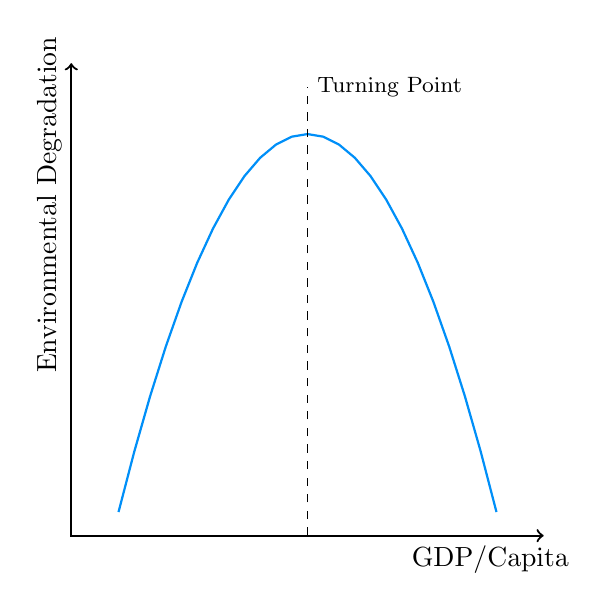
\begin{tikzpicture}[scale = 0.6]
\draw[thick, <->] (0,10) -- (0,0) -- (10,0);
\draw[thick, color1]  [domain = 1:9] plot (\x, {8.5 - .5*(\x - 5)^2});
\node [below right] at (7,0) {GDP/Capita};
\node[rotate=90, above] at (0,7) {Environmental Degradation};
\draw[dashed] (5,0) -- (5,9.5) node[right]{\footnotesize Turning Point};
\end{tikzpicture}
\end{minipage}
\begin{minipage}{0.48\textwidth}
\centering 
\caption{Application of the  EKC}
\includegraphics[width=0.9\textwidth]{figures/chapter2_figures/ekc.pdf}
\end{minipage}
Data from \cite{owidoutdoorairpollution} 
%https://ourworldindata.org/outdoor-air-pollution#outdoor-air-pollution-tends-to-rise-with-industrialization-before-falling
\end{figure}

Despite its quick adoption in the discipline and its continued use, the EKC has largely been discredited \citep{stern2004rise}. \cite{arrow1995economic} importantly note that the usual form of the EKC does not allow for any feedback between the environment and development, implicitly assuming that pollution and other forms of environmental degradation do not hinder economic development. 

\newpage
\subsection*{A.3\quad Appendix to Chapter 3: Ambient Air Pollution \& Electricity Generation}



\newpage
\subsection*{A.4\quad Appendix to Chapter 4: A Model of Emissions Pricing \& Environmental Inequality}

\begin{center}
    \singlespacing
    \renewcommand{\arraystretch}{1.5}
    \captionof{table}{Overview of Notation\label{notation}}
    \small
\begin{longtable}{c L{0.55\textwidth} C{0.15\textwidth} c}
    \hline\hline 
    Variable & Description & Determined & Source\\
    \hline \\[-1.8ex]
    \multicolumn{4}{l}{\emph{Indices \& Model Environment}}\\
    \hline 
    $i$ & Generator identifier & -- & -- \\
    $r$ & Region identifier & -- & -- \\
    $\ell$ & Transmission line identifier & -- & -- \\
    $m$ & Subregion or community identifier & -- & --\\ 
    $N$ & The number of generators & Exogenous & (1) \\
    $\mathcal{N}$ & Set of all generators; $\mathcal{N} = \{1, \ldots, N\}$ & Exogenous & (1) \\
    $\mathcal{N}_r$ & Set of all generators in region $r$ & Exogenous &  (1) \\
    $R$ & The number of regions & Exogenous &  (1) \\
    $\mathcal{L}$ & Set of all transmission lines & Exogenous &  (5) \\
    $M$ & Number of subregions or communities & Exogenous &  (3), (4)\\
    $T$ & Final period of the generation phase & Exogenous &  Chosen\\
    \\[-1.8ex]
    \multicolumn{4}{l}{\emph{Investment Phase}}\\
    \hline 
    $\mathcal{J}$ & Set of all investment options & Exogenous & Chosen\\
    $j_i$ & Generator $i$'s investment decision; $j_i \in \mathcal{J}$ & Endogenous & -- \\
    $j$ & Investment profile, $j = (j_1, j_2, \ldots, j_N)$ & Endogenous & -- \\
    $\rho_i^0$ & Generator $i$'s initial heat rate (BTU/kWh) & Exogenous & (1) \\
    $\rho_i$ & Generator $i$'s heat rate (BTU/kwh) & Endogenous & -- \\
    $\tilde{\delta}$ & Heat rate depreciation rate from the investment phase to the generation phase; $\tilde{\delta} \in (0, 1)$ & Exogenous & (10) \\
    $v_i$ & Generator $i$'s stochastic investment cost shock; $v_i > 0$ for all $i \in \mathcal{N}$ & Exogenous & Chosen \\
    $\gamma$ & Constant scalar in the investment cost function; $\gamma > 0$ & Exogenous & \\
    $\alpha$ & Scale parameter in the investment cost function; $\alpha > 0$ & Exogenous & \\
    $\Gamma (j_i, v_i)$ & Investment costs for generator $i$; a function of generator $i$'s investment choice $j_i$ and $i$' stochastic investment cost shock $v_i$ & Endogenous & -- \\
    $\Gamma (j \mid v)$ & Total investment costs for all generators; a function of the investment profile $j$ given a vector of all generator's stochastic investment cost shocks $v$ & Endogenous & -- \\
    $Q_t^e$ & $R$-dimensional vector of expected quantities demanded of electricity at time $t$ for each region (kWh) & Exogenous & (2)\\
    \\[-1.8ex]
    \multicolumn{4}{l}{\emph{Generation Phase}}\\
    \hline 
    $a_{it}$ & Operating decision of generator $i$ in period $t$; $a_{it} \in \{0, 1, \ldots, R\}$ where $a_{it} = r$ indicates that generator $i$ operates in period $t$ to sell its generation in region $r$ and $a_{it} = 0$ indicates that generator $i$ does not operate in period $t$ & Endogenous & -- \\
    $a_t$ & Profile of operating decisions in period $t$; $a_t = (a_{1t}, a_{2t}, \ldots, a_{Nt})$ & Endogenous & -- \\
    $\overline{q}_i$ & Generator $i$'s nameplate capacity (kW); the maximum rated generation of generator $i$ in an hour & Exogenous & (1) \\
    $q_{itr}$ & Generator $i$'s generation to be sold in region $r$'s wholesale electricity market at time $t$ (kWh) & Endogenous & -- \\
    $f_i$ & The primary fuel type of generator $i$; $f_i \in \{\text{Coal}, \text{Natural Gas}, \text{Oil}\}$ & Exogenous &  (1) \\
    $u_{f_i}$ & Unit cost of generator $i$'s fuel $f_i$ (\$/BTU) & Exogenous & (6), (7), (8)\\

    $e_{f_i}$ & Greenhouse gas emissions intensity of generator $i$'s fuel $f_i$ (tonnes CO$_2$e/BTU) & Exogenous & \\

    $\tau_r$ & Greenhouse gas emissions tax in region $r$ (\$/tonnes CO$_2$e) & Exogenous & (9) \\
    $P_{tr}$ & Price of electricity in region $r$'s wholesale market at time $t$ & Endogenous & -- \\
    $Q_{tr}$ & Quantity of electricity demanded in region $r$'s wholesale market at time $t$ & Exogenous &  (2) \\
    $C(a_t\mid j)$ & Total cost of generation in period $t$; a function of the profile if operating decisions $a_t$ given the profile of investment decisions $j$ & Endogenous & -- \\
    $MC(j)$ & Marginal cost matrix, $N \times R$; a function of the investment profile (vector) $j$; element in the $i$th row and $r$th column is $mc_{ir}$ & Endogenous & -- \\
    $G(a_t)$ & Generation matrix, $N \times R$; a function of the operating decision profile (vector) $a_t$; element in the $i$th row and $r$th column is $q_{itr}$ or $\overline{q}_i \1(a_{it} = r)$ & Endogenous & --\\
    $\rho^0$ & $N$-dimensional vector of heat rates in the absence of investment; the $i$th element is $\rho_i^0(1 + \tilde{\delta})$ & Endogenous & -- \\
    $D_{\rho^0 - j}$ & Diagonalized $N\times N$ matrix corresponding with the vector $\rho^0 - j$; for elements along the diagonal, the element in the $i$th row and $i$ column is $\rho_i = \rho_i^0(1 + \tilde{\delta}) - j_i$, all elements not along the diagonal are 0 & Endogenous & -- \\
    $U$ & Unit cost matrix, $N\times R$; the element in the $i$th row and $r$th column is generator $i$'s cost in region $r$ per BTU, $u_{f_i} + e_{f_i}\tau_r$ & Derived & -- \\
    $\overline{q}$ & $N$-dimensional vector of nameplate capacities; $\overline{q} = (\overline{q}_1, \overline{q}_2, \ldots, \overline{q}_N)$ & Derived & -- \\
    $D_{\overline{q}}$ & Diagonalized $N\times N$ matrix corresponding with the vector $\overline{q}$; for elements along the diagonal, the element in the $i$th row and $i$th column is $\overline{q}_i$, all elements not along the diagonal are 0 & Derived & -- \\
    $\1(a_t)$ & Operating decisions matrix, $N \times R$; the element in the $i$th row and $r$th column is $\1(a_{it} = r)$ & Endogenous & -- \\
    $\delta$ & Hourly discount factor, $\delta \in (0, 1)$ & Exogenous & (10)\\
    $y_{tr}$ & Net electricity exports for region $r$ at time $t$; alternatively, understood as a marginal power injection out of region $r$ at time $t$ & Endogenous & -- \\
    $PTDF_{r\ell}$ & Power transfer distribution factor on transmission line $\ell$ out of region $r$ & Exogenous & (5)\\
    $\text{Cap}_\ell$ & Maximum capacity of transmission line $\ell$ (kW) & Exogenous & (5)\\
    \\[-1.8ex]
    \multicolumn{4}{l}{\emph{The EI Gap}}\\
    \hline 
    $d$ & $M$-dimensional vector of communities' disadvantaged status; the $m$th element is 1 is $m$ is a disadvantaged community and 0 otherwise & Exogenous & (3), (4)\\
    $w$ & Local air pollutant identifier & -- & -- \\
    $e_i^w$ & Generator $i$'s emissions intensity of air pollutant $w$ (pounds/kWh) & Exogenous & (1)\\
    $w_{it}$ & Generator $i$'s emissions of air pollutant $w$ (lbs) & Endogenous & -- \\
    $\phi_w(w_{it}\mid i, t)$ & $M$-dimensional vector of the changes in the concentration of air pollutant $w$ across all $M$ communities resulting from $w_{it}$, the emissions of air pollutant $w$ from generator $i$ in time $t$ & Endogenous & -- \\
    $\Phi_w^1(T)$ & Average change in the concentration of pollutant $w$ for disadvantaged communities (elements of $d$ equal to 1) after $T$ periods & Endogenous & -- \\
    $\Phi_w^0(T)$ & Average change in the concentration of pollutant $w$ for non-disadvantaged communities (elements of $d$ equal to 0) after $T$ periods & Endogenous & -- \\
    $\text{EIGap}_w(T)$ & The environmental inequality gap after $T$ periods & Endogenous & -- \\
    \hline\hline
\end{longtable}
\fignote[1]{Table summarizes the notation used in Chapter 4. In general, lowercase letters without an index are profiles/vectors, plain-text uppercase letters denote matrices or the size of a set, and uppercase letters in the \texttt{mathcal} font are sets (e.g., $\mathcal{N}$). We denote the equilibrium of any variable as the variable with an asterisk. Derived variables are those that are a deterministic function of entirely exogenous variables. The source key for exogenous variables correspond with the data sources in Table \ref{data_sources}.}
\end{center}


\begin{center}
    \singlespacing
    \renewcommand{\arraystretch}{1.5}
    \captionof{table}{Data Sources Key\label{data_sources}}
    \small
    \begin{longtable}{c L{0.8\textwidth}}
        \hline\hline
        Source Key & Source Citation\\
        \hline \\[-3ex]
        (1) & United States Environmental Protection Agency (EPA). 2021. ``Emissions \& Generation Resource Integrated Database (eGRID), 2019" Washington, DC: Office of Atmospheric Protection, Clean Air Markets Division. Available from EPA's eGRID web site: \url{https://www.epa.gov/egrid}.\\ \\[-3ex]
        \hline \\[-3ex]
        (2) & United States Energy Information Administration (EIA). 2023. ``Hourly Electric Good Monitor'' Region Files. Available at: \url{https://www.eia.gov/electricity/gridmonitor/dashboard/electric_overview/US48/US48}\\ \\[-3ex]
        \hline \\[-3ex]
        (3) & United States Environmental Protection Agency. 2021 version. EJScreen. Census Tract-Level US Percentiles. Retrieved: 2023-03-03. Available at: \url{https://gaftp.epa.gov/EJSCREEN/2021/} \\ \\[-3ex]
        \hline \\[-3ex]
        (4) & California Office of Environmental Health \& Hazard Assessment (OEHHA). 2022. SB 535 Disadvantaged Communities. Retrieved: 2023-03-03. Available at: \url{https://oehha.ca.gov/calenviroscreen/sb535} \\ \\[-3ex]
        \hline \\[-3ex]
        (5) & Fowlie, Meredith, Petersen, Claire, and Reguant, Mar. Data and Code for: Border Carbon Adjustments When Carbon Intensity Varies Across Producers: Evidence from California. Nashville, TN: American Economic Association [publisher], 2022. Ann Arbor, MI: Inter-university Consortium for Political and Social Research [distributor], 2021-05-13. \url{https://doi.org/10.3886/E131024V1} \\ \\[-3ex]
        \hline \\[-3ex]
        (6) & United States Energy Information Administration. 2023. Natural Gas Electric Power Price. Source key: N3045. Available at: \url{http://www.eia.gov/dnav/ng/ng_pri_sum_a_epg0_peu_dmcf_m.htm} \\ \\[-3ex]
        \hline \\[-3ex]
        (7) & United States Energy Information Administration. 2023. Coal shipments to the electric power sector: price, by plant state. Available at: \url{https://www.eia.gov/coal/data/browser/} \\ \\[-3ex]
        \hline \\[-3ex]
        (8) & United States Energy Information Administration. 2023. Cushing, OK WTI Spot Price FOB (Dollars per Barrel). Source key: RWTC. Available at: \url{https://www.eia.gov/dnav/pet/hist/LeafHandler.ashx?n=PET&s=RWTC&f=M} \\ \\[-3ex]
        \hline \\[-3ex]
        (9) & California Air Resources Board. 2023. Cap-and-Trade Program Data Dashboard---Carbon Allowance Prices. Available at: \url{https://ww2.arb.ca.gov/our-work/programs/cap-and-trade-program/program-data/cap-and-trade-program-data-dashboard} \\ \\[-3ex]
        \hline \\[-3ex]
        (10) & Board of Governors of the Federal Reserve System (US), Market Yield on U.S. Treasury Securities at 10-Year Constant Maturity, Quoted on an Investment Basis [DGS10]. Retrieved: 2023-03-03 from FRED, Federal Reserve Bank of St. Louis. Available at: \url{https://fred.stlouisfed.org/series/DGS10} \\ \\[-3ex]
        \hline \\[-3ex]
        (11) & United States Energy Information Administration. 2022. Carbon Dioxide Emissions Coefficient. Available at: \url{https://www.eia.gov/environment/emissions/co2_vol_mass.php}\\ \\[-3ex]
        \hline\hline
    \end{longtable}
\end{center}

\newpage
\subsection*{A.5\quad Appendix to Chapter 5: Carbon Pricing \& Air Pollution Disparities in California}



\end{document}